\documentclass[mathserif]{beamer}
\usepackage{accents}
\usepackage{algorithm}
\usepackage{algorithmic}
\usepackage{amsmath}
\usepackage{booktabs}
\usepackage{color}
\usepackage{colortbl}
\usepackage{ifdraft}
\usepackage{mathrsfs}
\usepackage{mathtools}
\usepackage[normalem]{ulem}
\usepackage[labelformat=empty]{caption}
\usepackage[warn]{makecmds}
\usepackage{siunitx}
\usepackage{appendixnumberbeamer}
\mathtoolsset{showonlyrefs,showmanualtags}
\usetheme[secheader]{pecostalk}
\graphicspath{{figs/}}
\usepackage[sort&compress]{natbib}
\providecommand\newblock{} % DANGER, natbib/beamer incompatible
\renewcommand{\newblock}{} % DANGER, hack them to be compatible
% Custom commands used for notational purposes
%%%%%%%%%%%%%%%%%%%%%%%%%%%%%%%%%%%%%%%%%%%%%%

% Things which should behave like operators re: spacing
\DeclareMathOperator{\covariance}{Cov}
\DeclareMathOperator{\trace}{tr}
\DeclareMathOperator{\variance}{Var}

% Requires the `ifdraft' package be defined
\newcommand{\draftonly}[1]{\ifdraft{#1}{}}

% Source term from integral constraints
\newcommand{\Cs}{\ensuremath{\mathcal{C}}}

% Imaginary unit
\newcommand{\ii}{\ensuremath{\mathrm{i}}}

% Knudsen number with optional subscript
\newcommand{\Knudsen}[1][]{\ensuremath{\mbox{Kn}_{#1}}}

% Mach number with optional subscript
\newcommand{\Mach}[1][]{\ensuremath{\mbox{Ma}_{#1}}}

% Partial-something-by-partial-something-else derivatives
% Negative thin spaces added because Charter has too much space here
\newcommand{\pp}[2]{\frac{\partial\!{#1}}{\partial\!{#2}}}

% Prandtl number with optional subscript
\newcommand{\Prandtl}[1][]{\ensuremath{\mbox{Pr}_{#1}}}

% A reference value; a quantity less a reference value
\newcommand{\reference}[1]{\ensuremath{\left\{#1\right\}_{0}}}
\newcommand{\lessreference}[1]{\ensuremath{\left({#1}-\reference{#1}\right)}}

% Reynolds number with optional subscript
\newcommand{\Reynolds}[1][]{\ensuremath{\mbox{Re}_{#1}}}

% Source term from slow derivative
\newcommand{\Ssd}{\ensuremath{\mathcal{S}}}

% The symmetric part of a tensor
\newcommand{\symmetricpart}[1]{\ensuremath{\operatorname{sym}\left(#1\right)}}

% Denote something as a tensor
\newcommand{\tensor}[1]{\ensuremath{\accentset{\leftrightarrow}{#1}}}

% Take the transpose
\newcommand{\trans}[1]{{#1}^{\mathsf{T}}}

% The expectation operator
\newcommand{\expect}[1]{\operatorname{\mathbb{E}}\left[#1\right]}

% Victor's macros for notation
\newcommand{\fav}  [1] {\ensuremath{\widetilde{#1}}}  % Favre average
\newcommand{\fluc} [1] {\ensuremath{#1'}}             % Reynolds fluctuations
\newcommand{\ffluc}[1] {\ensuremath{#1''}}            % Favre fluctuations
\newcommand{\func} [2] {\ensuremath{#1 \! \left(#2\right)}}  % Function, IV
\newcommand{\mean} [1] {\ensuremath{\overline{#1}}}     % mean
           % Custom commands loaded from here

% http://tex.stackexchange.com/questions/110388
% I want 1e-2 not 1x10^{-2} from siunitx
\sisetup{output-exponent-marker=\ensuremath{\mathrm{e}}}

\setbeamertemplate{itemize/enumerate body begin}{\small}
\setbeamertemplate{itemize/enumerate subbody begin}{\footnotesize}

\makecommand{\z}{\phantom{0}}  % Facilitates column alignment
\makecommand{\Z}{\phantom{.0}} % Ditto
\makecommand{\n}{\phantom{$-$}}  % Ditto
\makecommand{\c}[1]{}          % Comment out material

\date{5 August 2014}
\author[Rhys Ulerich]{Rhys Ulerich}
\institute{Center for Predictive Engineering and Computational Sciences\\
           Institute for Computational Engineering and Sciences\\
           The University of Texas at Austin}
\title[Reducing Aerothermal Heating Uncertainty]{%
    \mbox{Reducing Turbulence- and Transition-Driven Uncertainty}
    \mbox{in Aerothermodynamic Heating Predictions}
    \mbox{for Blunt-Bodied Reentry Vehicles}
}

\begin{document}
%%%%%%%%%%%%%%%%%%%%%%%%%%%%%%%%%%%%%%%%%%%%%%%%%%%%%%%%%%%%%%%%%%%%%%%%%%%%%%

%===============================================================================
% Title page
\begin{frame}
%
\titlepage{}
\begin{columns}[]
  \begin{column}{0.1\linewidth}
    \begin{flushleft}
      
\includegraphics[scale=0.07]{circle-logo}\\
    \end{flushleft}
  \end{column}
  %
  \begin{column}{0.8\linewidth}
    \begin{center}
      \tiny{\emph{%
          Acknowledgment: This material is based upon work supported by the
          Department of Energy [National Nuclear Security Administration] under
          Award Number [DE-FC52-08NA28615].
      }}
    \end{center}
  \end{column}
  %
  \begin{column}{0.1\linewidth}
    \begin{flushright}
      
\includegraphics[scale=0.1]{asc_logo}\\
    \end{flushright}
  \end{column}
\end{columns}
%
\end{frame}

%===============================================================================
\begin{frame}{Thank you}
\begin{center}
%Drs\@. Biros, Clemens, Demkowicz, Oliver, van de Geijn
\begin{columns}
   \begin{column}{0.44\linewidth}
      Dr\@. Robert D. Moser, Supervisor \\
      Dr\@. George Biros \\
      Dr\@. Noel T. Clemens
  \end{column}
  \begin{column}{0.44\linewidth}
      Dr\@. Leszek F. Demkowicz \\
      Dr\@. Todd A. Oliver \\
      Dr\@. Robert van de Geijn
  \end{column}
\end{columns}
\vspace{2em}
\pause{}
\begin{columns}[t]
    \begin{column}{0.32\linewidth}
        Paul Bauman \\
        Michael Borden \\
        Henry Chang \\
        Jesse Chan \\
        Truman Ellis \\
        Kemelli Estacio-Hiroms \\
        Omar Al Hinai
    \end{column}
    \begin{column}{0.32\linewidth}
        Benjamin Kirk \\
        Thomas Kirschenmann \\
        Myoungkyu Lee \\
        Nicholas Malaya \\
        Damon McDougall \\
        Craig Michoski \\
        Rebecca Morrison \\
        Nathan Roberts
    \end{column}
    \begin{column}{0.32\linewidth}
        Oleg Schilling \\
        Karl Schulz \\
        Christopher Simmons \\
        Roy Stogner \\
        Victor Topalian \\
        Jesse Windle \\
        Shan Yang
    \end{column}
\end{columns}
\vspace{2em}
\pause{}
Michelle, Ozark, \& Oxford
\end{center}
\end{frame}

%===============================================================================
\begin{frame}[noframenumbering]
    \frametitle{Outline}
    \tableofcontents
\end{frame}

%%%%%%%%%%%%%%%%%%%%%%%%%%%%%%%%%%%%%%%%%%%%%%%%%%%%%%%%%%%%%%%%%%%%%%%%%%%%%%%%
\section[Introduction]{Aerothermodynamic Heating Predictions\newline{}for Blunt-Bodied Reentry Vehicles}
%%%%%%%%%%%%%%%%%%%%%%%%%%%%%%%%%%%%%%%%%%%%%%%%%%%%%%%%%%%%%%%%%%%%%%%%%%%%%%%%

% Show outline at beginning of relevant sections
%\AtBeginSection[]
%{
%   \begin{frame}[noframenumbering]
%       \frametitle{Outline}
%       \tableofcontents[currentsection]
%   \end{frame}
%}
\AtBeginSubsection[]
{%
  \begin{frame}<*>{Outline}
    \tableofcontents[currentsection,currentsubsection]
  \end{frame}
}

%===============================================================================
\begin{frame}
\frametitle{NASA Orion Multi-Purpose Crew Vehicle (MPCV)}
\begin{figure}[h]
  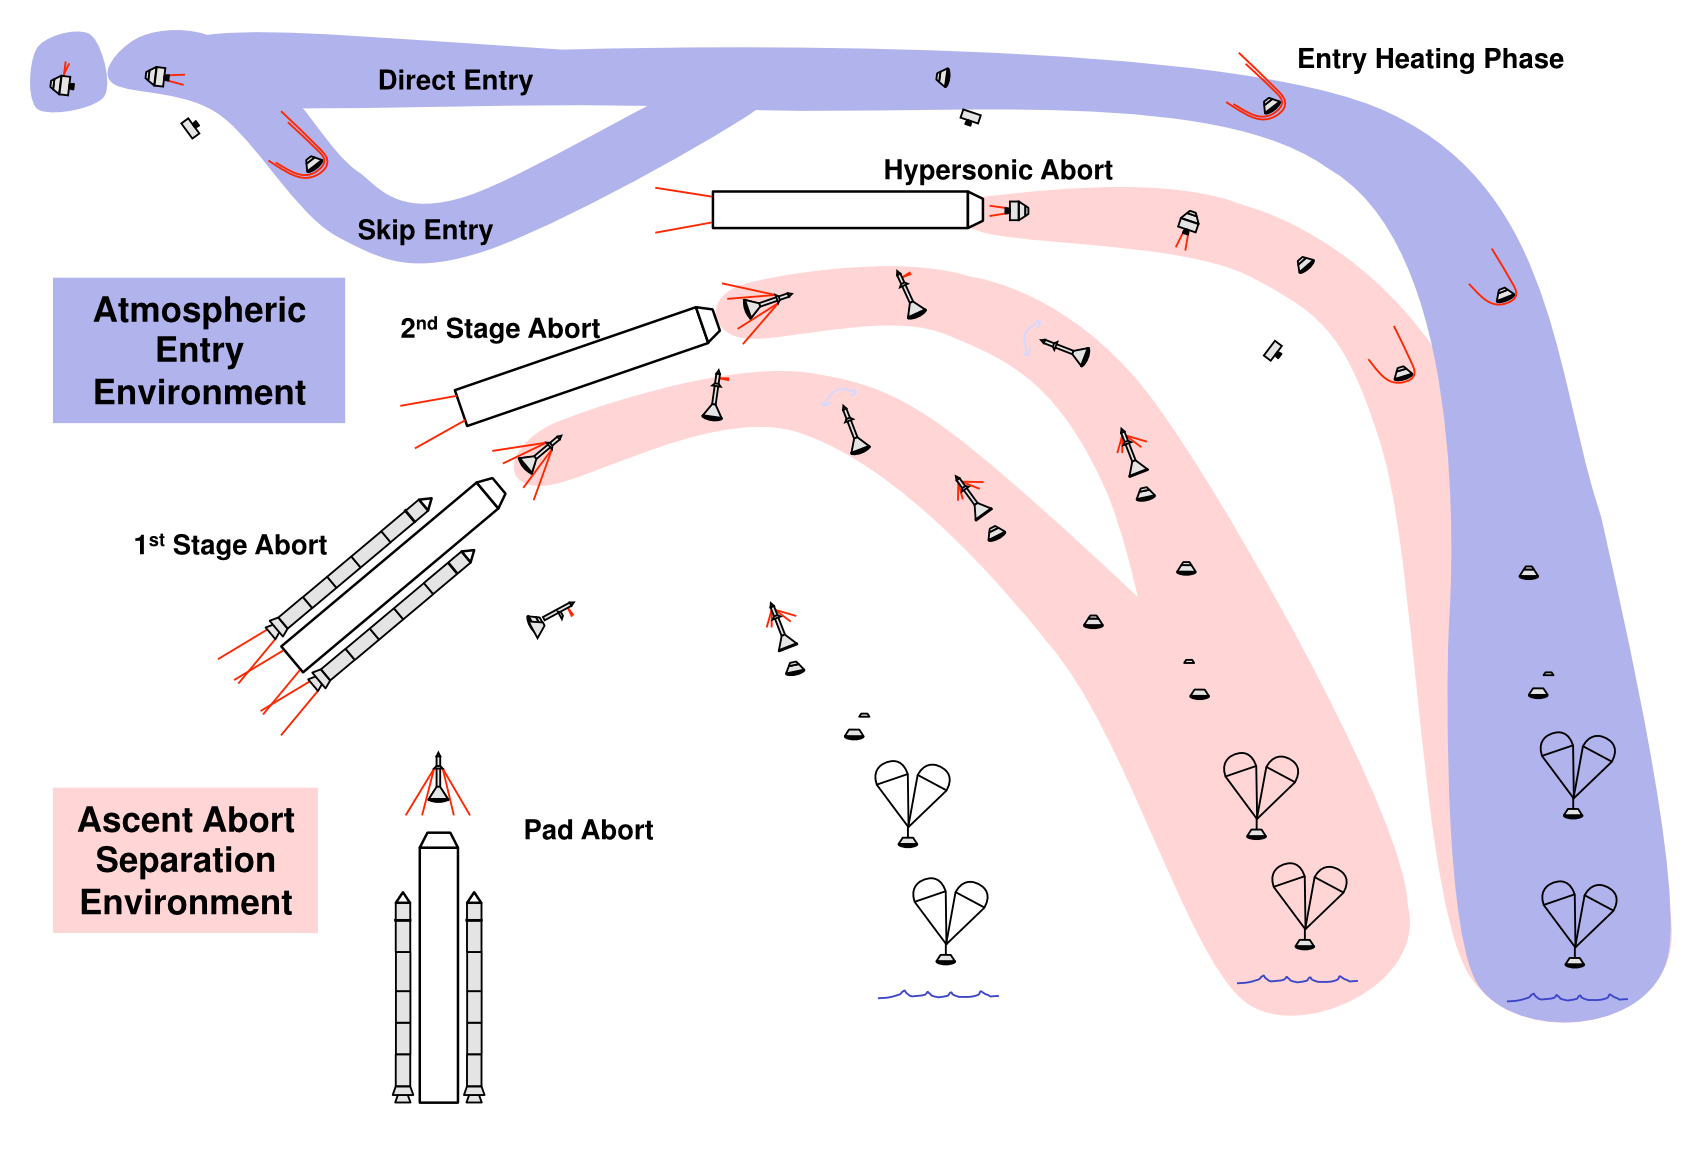
\includegraphics[width=\textwidth]{ResponsibleFlightRegimes_Raster}
  \vspace{-3em}
  \small
  \begin{flushright}
    courtesy NASA
  \end{flushright}
\end{figure}
\end{frame}

%===============================================================================
\begin{frame}
\begin{figure}[h]
  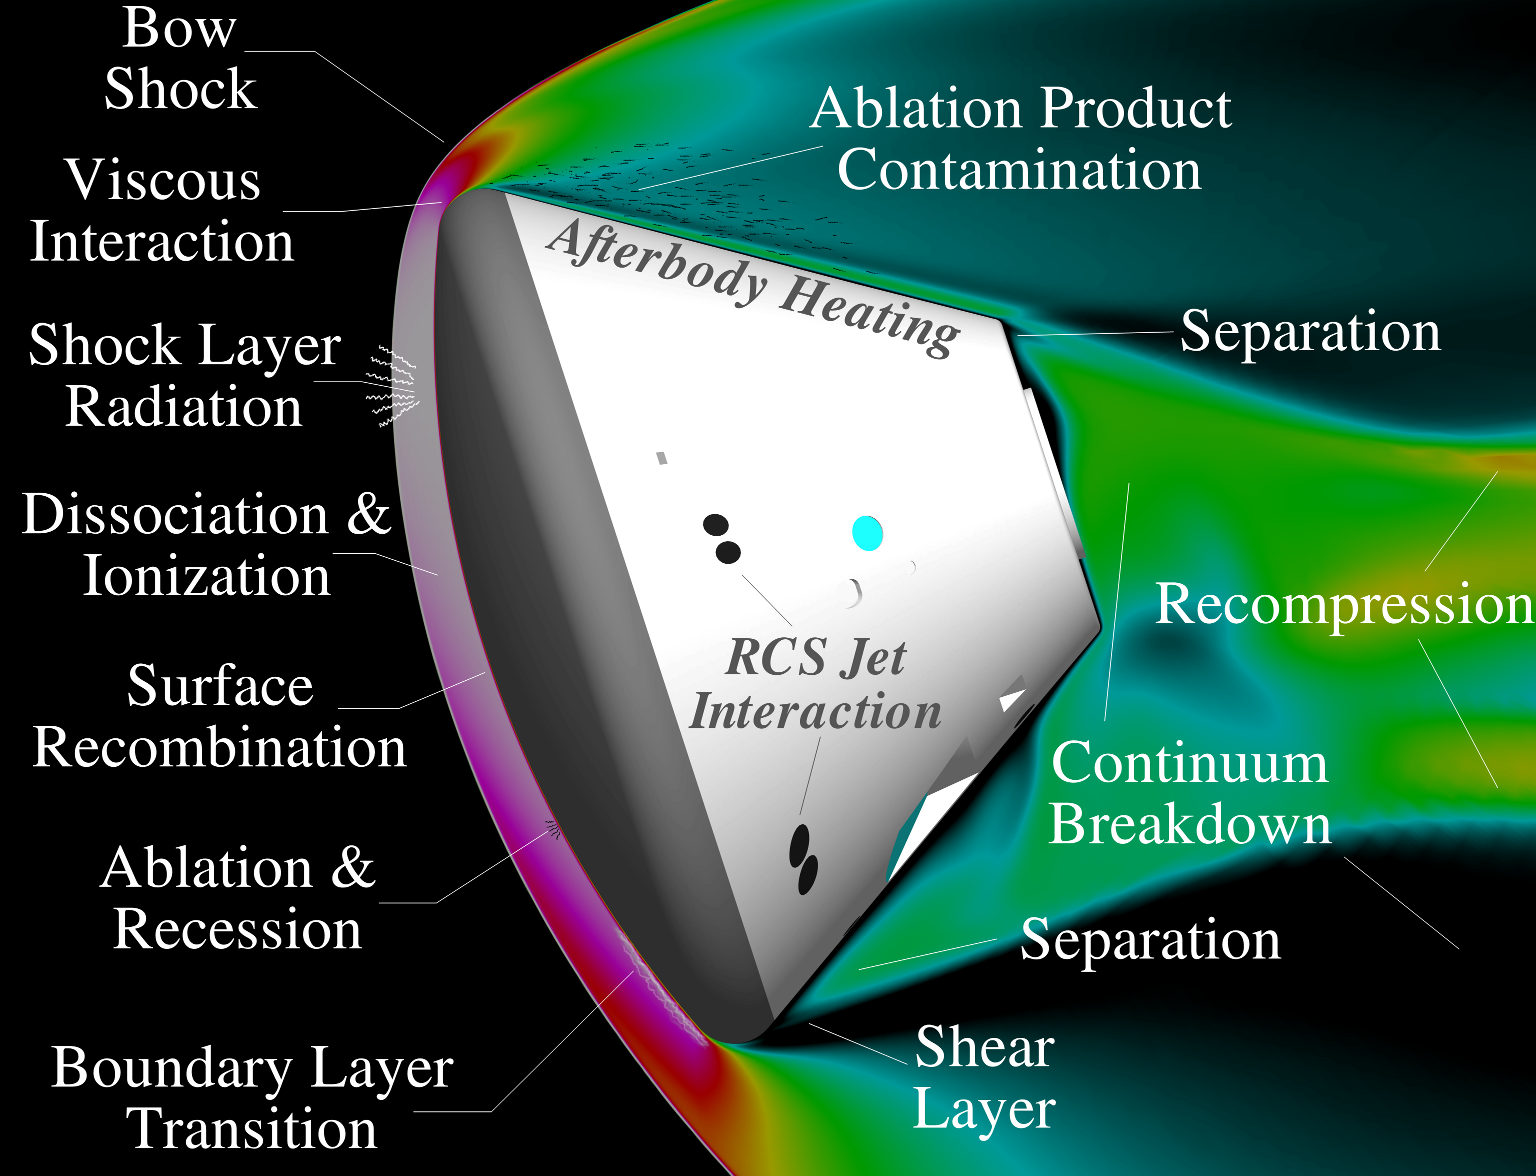
\includegraphics[width=0.58\textwidth]{Capsule_image_updated}
\end{figure}
  \begin{block}{Survival of a blunt-bodied reentry vehicle depends upon}
    \small
    \begin{itemize}
    \item Recession rate of ablative thermal protection system\\
          (throughout peak heating regime of flight trajectory)
    \item Local peak heat flux to after-body
    \end{itemize}
  \end{block}
\end{frame}

%===============================================================================
\begin{frame}
\begin{figure}[h]
  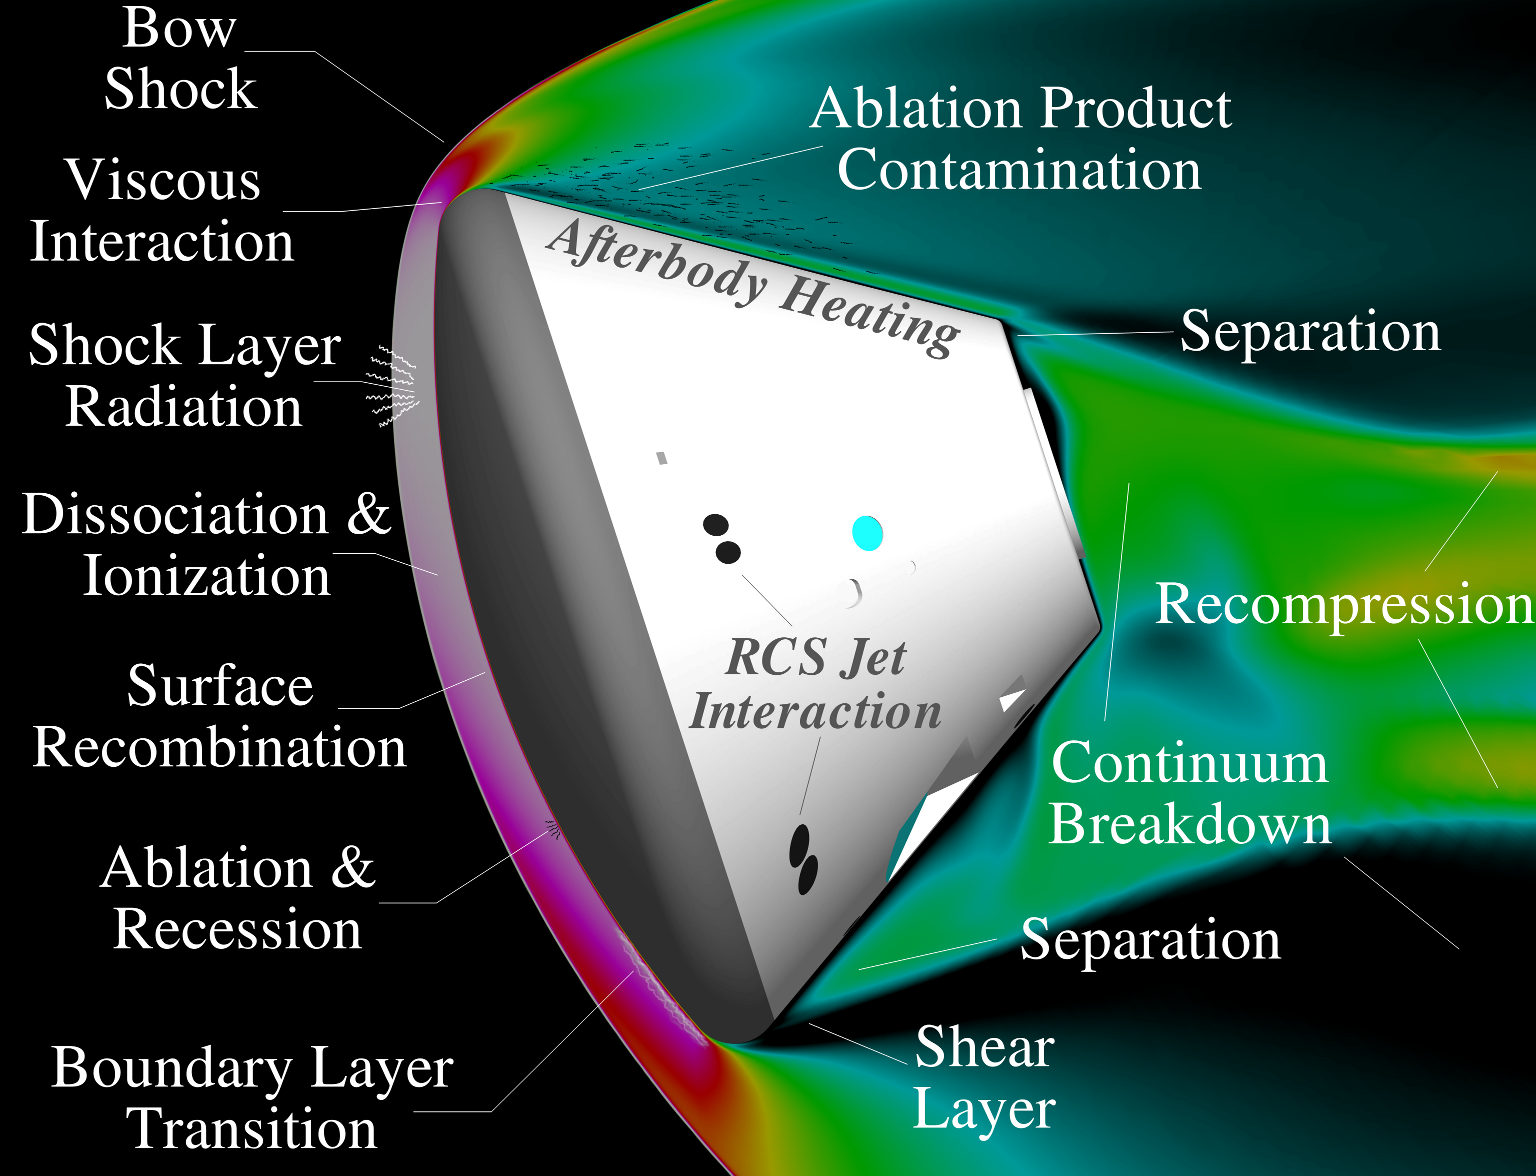
\includegraphics[width=0.58\textwidth]{Capsule_image_updated}
\end{figure}
\begin{block}{Among other things, ablation rate depends upon}
  \small
  \begin{description}
  \item[Turbulence] Relative to laminar behavior, turbulent mixing
                    intensifies heating by enhancing momentum,
                    energy, and chemical species
                    transport
  \item[Transition] Transition from laminar-to-turbulent flow
                    determines where exactly this intensified heating
                    occurs on the ablative heat shield
  \end{description}
\end{block}
\end{frame}

%%%%===============================================================================
%%%\begin{frame}{Motivating concepts that are out of scope}
%%%\begin{itemize}
%%%  \item Reentry vehicle ablation rate predictions\\
%%%        {\footnotesize \citet{Bauman2011Loose, Stogner2011Uncertainty}}
%%%  \item Bayesian turbulence model calibration\\
%%%        {\footnotesize \citet{RESS-2010, ETC13-2011, Oliver2012Accounting}}
%%%  \item Turbulence model application, assessment, and development\\
%%%        {\footnotesize \citep{Durbin2011Statistical, Pope2000Turbulent, Chassaing2010Variable, Wilcox2006Turbulence}}
%%%  \item Classical laminar-to-turbulent transition modeling\\
%%%        {\footnotesize See review by \citet{Federov2011Transition}}
%%%\end{itemize}
%%%\end{frame}

%%%%%%%%%%%%%%%%%%%%%%%%%%%%%%%%%%%%%%%%%%%%%%%%%%%%%%%%%%%%%%%%%%%%%%%%%%%%%%%%
\section{Reducing Turbulence-Driven Uncertainty}
%%%%%%%%%%%%%%%%%%%%%%%%%%%%%%%%%%%%%%%%%%%%%%%%%%%%%%%%%%%%%%%%%%%%%%%%%%%%%%%%

%===============================================================================
\subsection{Motivation and Background}
%===============================================================================

%===============================================================================
\begin{frame}{%
  Ablation rate predictions highly sensitive to turbulence\\
  and therefore highly dependent on calibration data
}
\begin{columns}[c,onlytextwidth]
\begin{column}{.49\linewidth}
  \begin{center}
    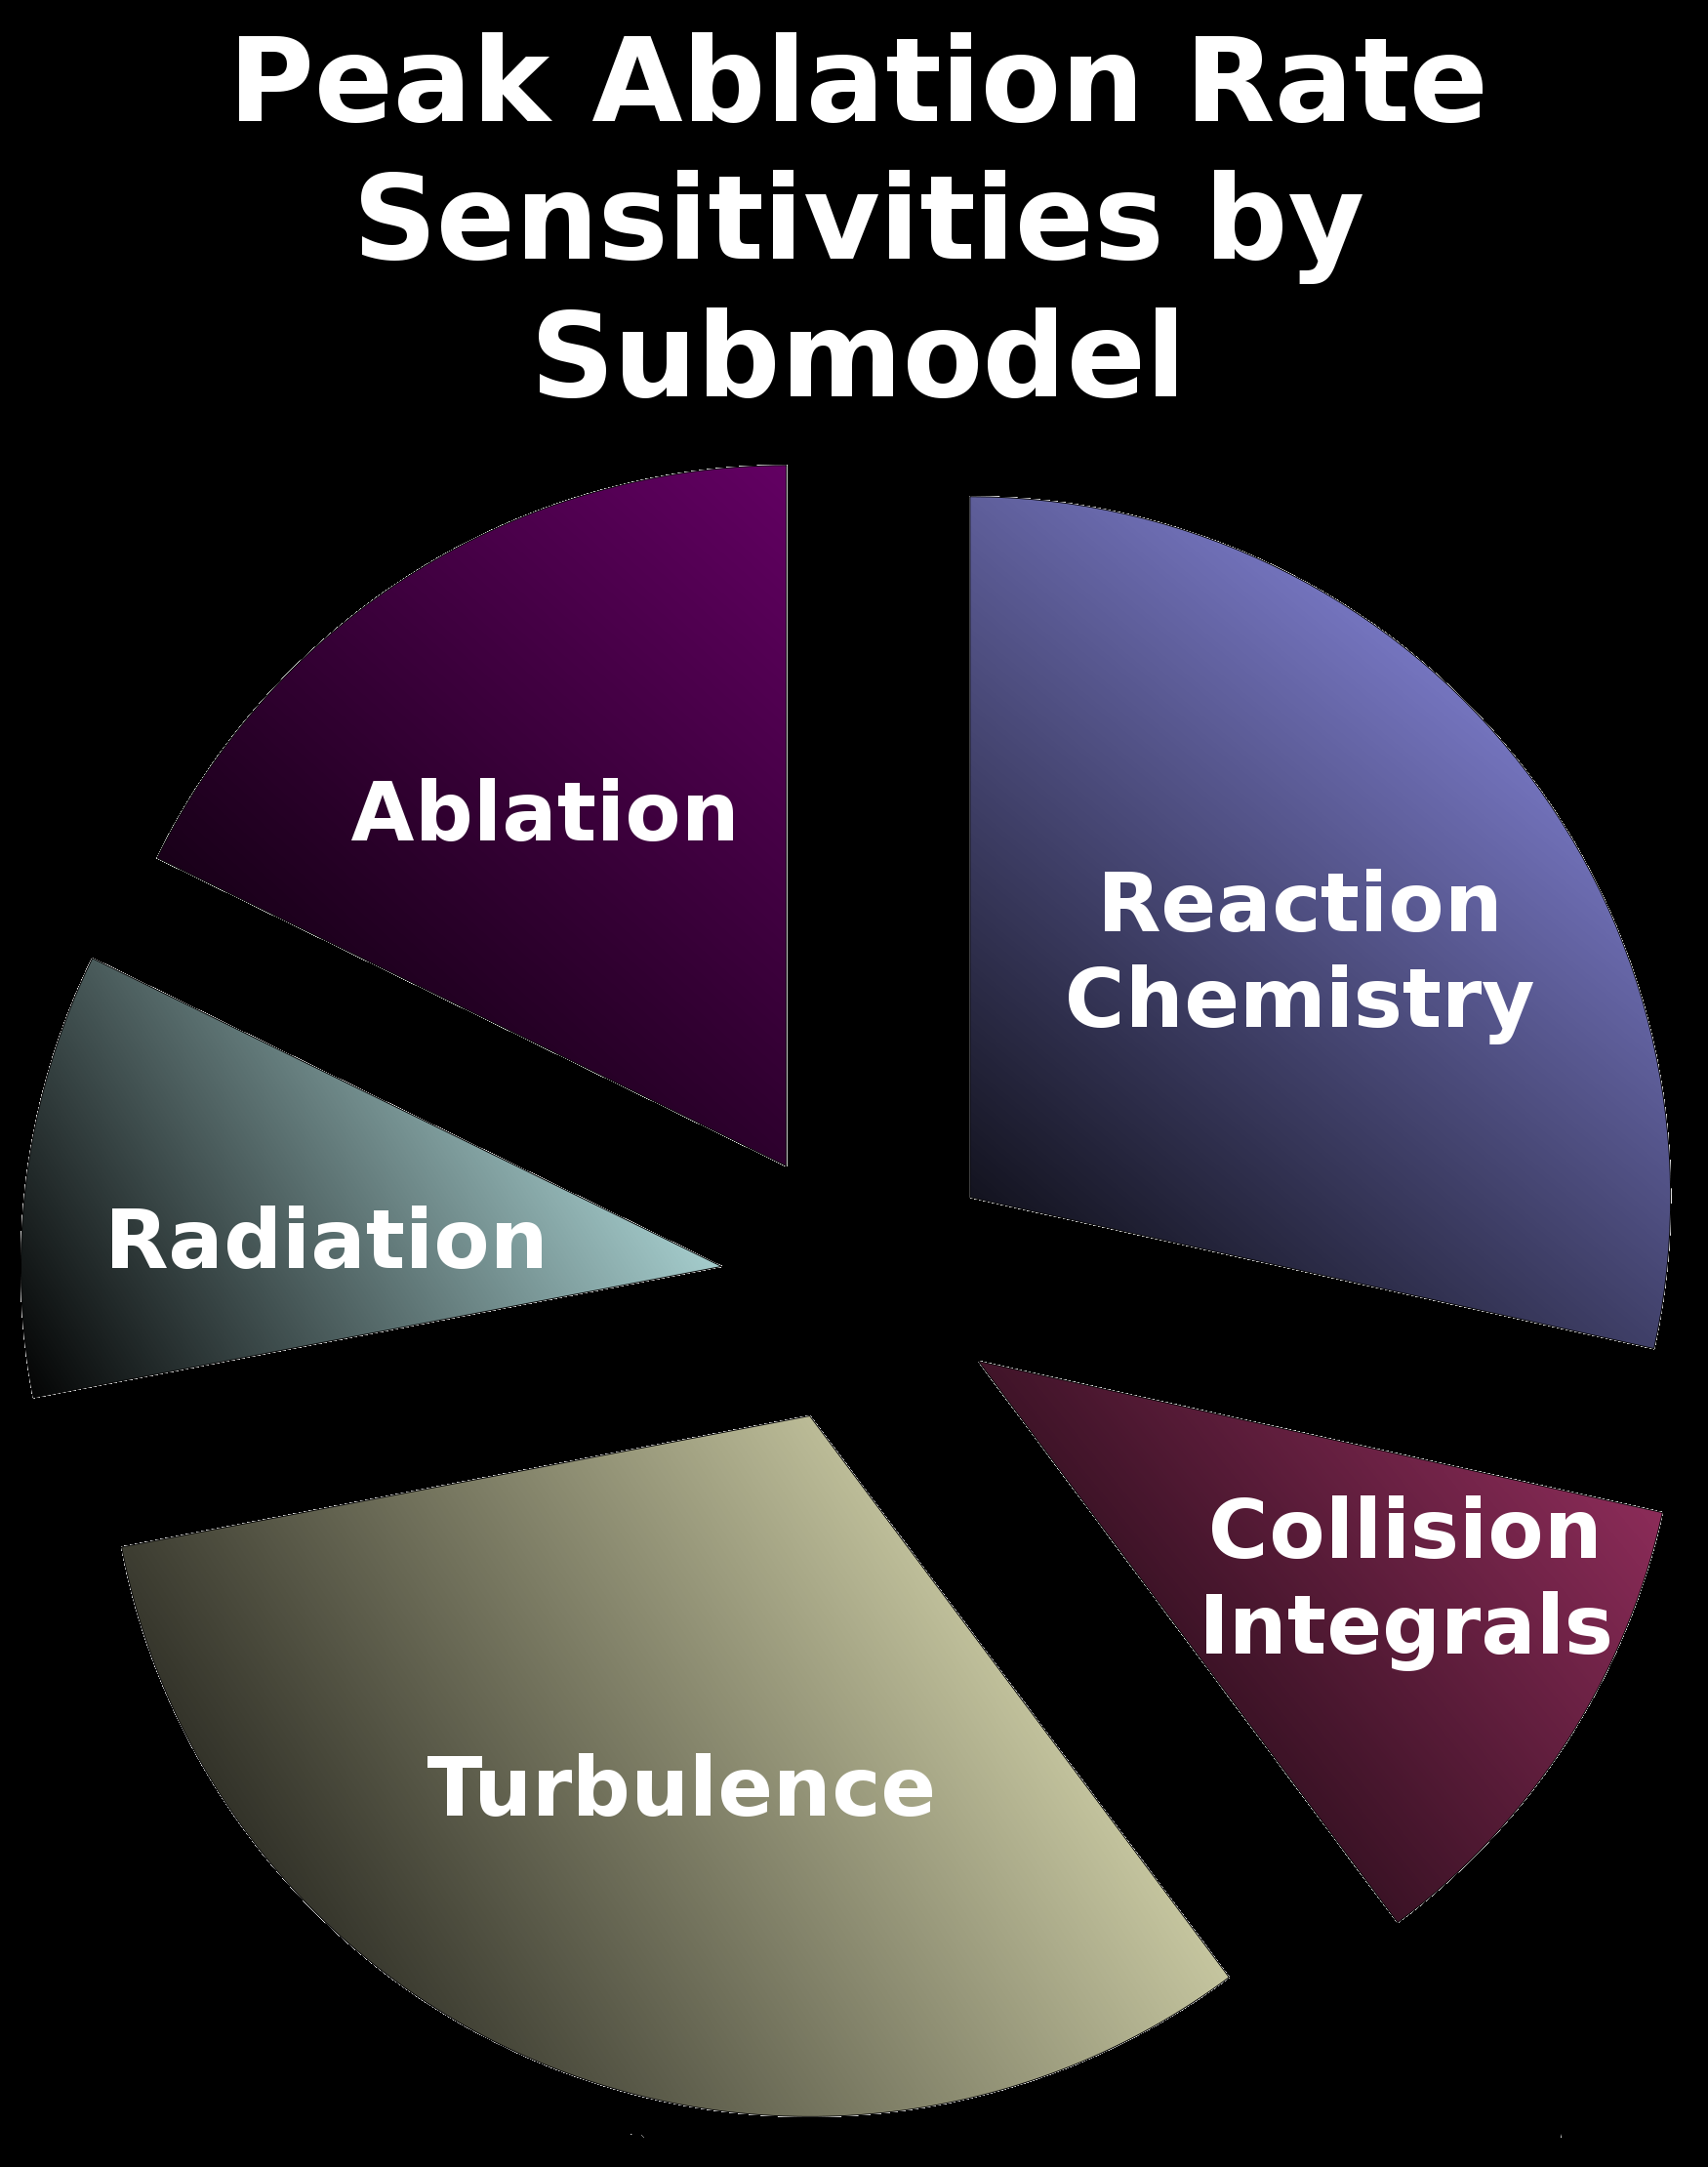
\includegraphics[width=0.85\linewidth]{sensitivity_by_submodel_portrait}
    \\
    from \citet{Stogner2011Uncertainty}
  \end{center}
\end{column}
\begin{column}{.49\linewidth}
  Eddy viscosity-based turbulence models widely used in engineering:
  \begin{itemize}
    \item Models well-known to be\\imperfect and unreliable
    \item Higher-fidelity approaches computationally intractable
  \end{itemize}
  \vfill
  Turbulence models contain imperfectly known parameters
  \begin{itemize}
    \item Must be calibrated using relevant, trusted data
    \item Prediction uncertainty limited by effectiveness of calibration
  \end{itemize}
\end{column}
\end{columns}
\end{frame}

%%===============================================================================
%\begin{frame}{\dots{}therefore dependent on turbulence model calibration}
%\begin{columns}[c,onlytextwidth]
%\begin{column}{.45\linewidth}
%  Turbulence models contain {\color{red}imperfectly known parameters}:
%  \begin{itemize}
%    \item Must be calibrated using relevant, trusted data
%    \item Prediction uncertainty limited by effectiveness of calibration
%  \end{itemize}
%\end{column}
%\begin{column}{.52\linewidth}
%\begin{block}{Example, $k$-$\omega$ (Menter/SST)}
%\resizebox{.93\hsize}{!}{\parbox{\linewidth}{
%\begin{align*}
%\pp{\bar{\rho}}{t} + \pp{}{x_i} (\bar{\rho}\tilde{u}_i) &= 0
%\\
%\pp{}{t} \left(\bar{\rho} \tilde{u}_i \right) + \pp{}{x_j} \left(\bar{\rho} \tilde{u}_j \tilde{u}_i  \right) &= - \, \pp{\bar{p}}{x_i} + \pp{}{x_j}\left( 2 (\bar{\mu} + \mu_t) \tilde{S}_{ji} - \frac{2}{3} \bar{\rho} k \delta_{ji} \right)
%\\
%\pp{}{t} \left( \bar{\rho} \tilde{E} \right) + \pp{}{x_j} \left( \bar{\rho} \tilde{u}_j \tilde{H} \right) &= \pp{}{x_j} \left( 2 (\bar{\mu} + \mu_t) \tilde{S}_{ji} \tilde{u}_i - \frac{2}{3} \bar{\rho} k \delta_{ji} \tilde{u}_i \right)
%\\
%&{}+ \pp{}{x_j} \left[ \left( \frac{\bar{\mu}}{Pr} + \frac{\mu_t}{Pr_t} \right) \pp{\tilde{h}}{x_j} \right] + \pp{}{x_j} \left[ \left( \bar{\mu} + \sigma_k \mu_t \right) \pp{k}{x_j} \right]
%\\
%\pp{}{t} (\bar{\rho} k) + \pp{}{x_j}(\bar{\rho} \tilde{u}_j k) &= \left( 2 \mu_t \tilde{S}_{ij}  - \frac{2}{3} \bar{\rho} k \delta_{ij} \right) \pp{\tilde{u}_i}{x_j} - {\color{red}\beta^*} \bar{\rho} \omega k + \pp{}{x_j} \left[ (\bar{\mu} + \sigma_k \mu_t) \pp{k}{x_j} \right]
%\\
%\pp{}{t}(\bar{\rho} \omega) + \pp{}{x_j}(\bar{\rho} \tilde{u}_j \omega) &= \frac{\alpha}{\nu_t} \left( 2 \mu_t \tilde{S}_{ij}  - \frac{2}{3} \bar{\rho} k \delta_{ij} \right) \pp{\tilde{u}_i}{x_j} - \beta \bar{\rho} \omega^2
%\\
%&{}+ \pp{}{x_j} \left[ (\bar{\mu} + \sigma_{\omega} \mu_t) \pp{\omega}{x_j} \right] + 2 (1 - F_1) \bar{\rho} {\color{red} \sigma_{\omega 2}} \frac{1}{\omega} \pp{k}{x_j} \pp{\omega}{x_j}
%\end{align*}
%\begin{gather*}
%\bar{\mu} = \mu_0 \left( \frac{\tilde{T}}{T_0} \right)^{3/2} \frac{T_0 + S}{\tilde{T} + S}, \quad \tilde{S}_{ij} = \tilde{s}_{ij} - \frac{1}{3} \tilde{s}_{kk} \delta_{ij}, \quad \tilde{s}_{ij} = \frac{1}{2} \left( \pp{\tilde{u}_i}{x_j} + \pp{\tilde{u}_j}{x_i} \right),
%\\
%\bar{p} = \bar{\rho} R \tilde{T}, \quad \tilde{E} = \tilde{e} + \frac{1}{2} \tilde{u}_i \tilde{u}_i + k, \quad \tilde{e} = c_v \tilde{T}, \quad \tilde{H} = \tilde{h} + \frac{1}{2} \tilde{u}_i \tilde{u}_i + k, \quad \tilde{h} = c_p \tilde{T} = \tilde{e} + \frac{\bar{p}}{\bar{\rho}}\,
%\\
%\mu_t = \frac{{\color{red} a_1} \bar{\rho} k}{\max( {\color{red} a_1} \omega, \Omega F_2 )}, \quad \Omega = \sqrt{2 \tilde{\Omega}_{ij} \tilde{\Omega}_{ij} }, \quad F_2 = \tanh( \arg_2^2 ), \quad \arg_2 = \max \left( \frac{2 \sqrt{k}}{0.09 \omega d}, \frac{500 \tilde{\nu}}{d^2 \omega} \right),
%\\
%\sigma_k = F_1 {\color{red} \sigma_{k1}} + (1-F_1) {\color{red} \sigma_{k2}}, \quad \sigma_{\omega} = F_1 {\color{red} \sigma_{\omega 1}} + (1-F_1) {\color{red} \sigma_{\omega 2}}, \quad \beta = F_1 {\color{red} \beta_1} + (1-F_1) {\color{red} \beta_2}
%\\
%\alpha = F_1 \alpha_1 + (1 - F_1) \alpha_2, \quad \alpha_1 = \frac{\color{red} \beta_1}{\color{red} \beta^*} - {\color{red} \sigma_{\omega 1}} \frac{{\color{red} \kappa}^2}{\sqrt{\color{red}\beta^*}}, \quad \alpha_2 = \frac{\color{red} \beta_2}{\color{red} \beta^*} - {\color{red} \sigma_{\omega 2}} \frac{{\color{red} \kappa}^2}{\sqrt{\color{red} \beta^*}},
%\\
%F_1 = \tanh ( \arg_1^4 ), \quad \arg_1 = \min \left( \arg_2, \frac{4 \bar{\rho} {\color{red} \sigma_{\omega 2}} k}{\mathrm{CD}_{k \omega} d^2} \right), \quad \mathrm{CD}_{k \omega} = \max \left( 2 \bar{\rho} {\color{red} \sigma_{\omega 2}} \frac{1}{\omega} \pp{k}{x_j} \pp{\omega}{x_j}, 0 \right)
%\end{gather*}
%}}%resizebox
%\end{block}
%\end{column}
%\end{columns}
%\end{frame}

%%===============================================================================
%\begin{frame}{Effective calibration demands high-quality data\dots}
%             {(illustrated from a Bayesian model calibration perspective)}
%By Bayes' theorem, model parameters $\theta$ are updated using data $d$:
%\begin{align}
%  p_\text{post}\!\left(\theta|d\right)
%  &\propto
%  L\!\left(d|\theta\right)
%  p_\text{prior}\!\left(\theta\right)
%\end{align}
%%
%\vfill
%%
%Calibration data measurement uncertainty is accounted for within
%$L\!\left(d|\theta\right)$:
%\begin{itemize}
%  \item Larger data uncertainties cause less certain predictions
%  \item Inaccurately small data uncertainties poison predictions
%\end{itemize}
%%
%\vfill
%%
%We say turbulence calibration data is ``high quality'' whenever
%\begin{itemize}
%  \item it has accurately quantified measurement uncertainties, and
%  \item when those measurement uncertainties are small, and
%  \item it satisfies remaining criteria set forth by \citet{Settles1991Hypersonic}
%\end{itemize}
%%
%\end{frame}

%===============================================================================
\begin{frame}{Effective calibration demands high-quality data\\
              but data relevant to blunt-bodied vehicle reentry is scarce}
%
High-quality data from the heating prediction scenario is nonexistent
\vfill
Seek boundary layer data from conditions representative of reentry\\
and use surface heat flux as a surrogate for ablation rate:
\begin{enumerate}
 \item Cold wall
 \item Wall blowing
 \item Favorable pressure gradients
 \item Chemically reacting species under high-enthalpy conditions
 \item Convex surface curvature
 \item Surface roughness
\end{enumerate}
\vfill
High-quality, $\Mach>1$ turbulent boundary layer data generally scarce\\
Scarcity compounded by adding any one of the above conditions
\end{frame}

%===============================================================================
\begin{frame}{Direct numerical simulation (DNS)}
\begin{columns}[c]
  \begin{column}{.50\textwidth}
    DNS solves the complete Navier--Stokes equations:
    \begin{itemize}
      \item Must resolve all scales of motion
      \item Becomes painfully expensive as Reynolds number increases
      \item Expense mainly comes from resolving small, dissipative scales
    \end{itemize}
  \end{column}
  \begin{column}{.45\textwidth}
    \begin{block}{Isotropic DNS expense}
      \begin{footnotesize}
      \begin{align*}
        &L
        &&\text{Macro length scale}
        \\
        &\eta \equiv \left(\frac{\nu^{3}}{\epsilon}\right)^{1/4}
        &&\text{Kolmogorov scale}
        \\
        &N \sim \frac{L}{\eta} \sim \Reynolds[L]{}^{3/4}
        &&\text{1D resolution}
        \\
        &N^{3} \sim \Reynolds[L]{}^{9/4}
        &&\text{3D resolution}
        \\
        &\Reynolds[L]{}^{4}
        &&\text{3D w/ CFL}
      \end{align*}
      \end{footnotesize}
    \end{block}
  \end{column}
\end{columns}
%\vfill
%\begin{block}{Other less expensive approaches require additional modeling:}
%  \begin{itemize}
%    \item RANS/FANS solves for Navier--Stokes' first moment
%    \item LES solves filtered Navier--Stokes for only the large scales
%  \end{itemize}
%\end{block}
\vfill
    Reentry scenario is accessible by DNS:
    $\Reynolds[\theta]{}\lessapprox 700$
\end{frame}

%%%%===============================================================================
%%%\begin{frame}{Two canonical problems in DNS}
%%%\begin{block}{Channel Flow}
%%%  \begin{columns}[c]
%%%    \begin{column}{0.50\linewidth}
%%%      \begin{center}
%%%        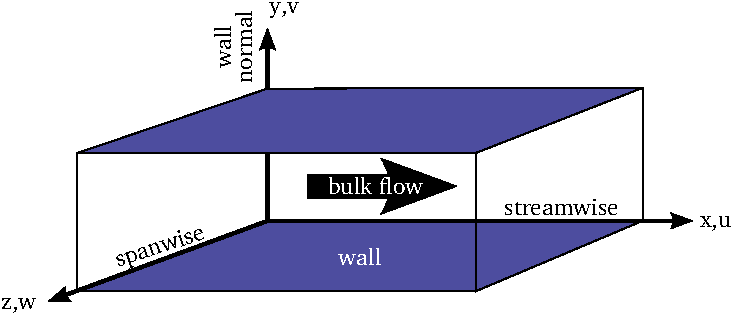
\includegraphics[width=.99\linewidth]{ChannelSchematic}
%%%      \end{center}
%%%    \end{column}
%%%    \begin{column}{0.41\linewidth}
%%%        Forcing the momentum equation drives mean streamwise flow\\
%%%        \vspace{\baselineskip}
%%%        Statistically one-dimensional
%%%    \end{column}
%%%  \end{columns}
%%%\end{block}
%%%\begin{block}{Flat Plate}
%%%  \begin{columns}[c]
%%%    \begin{column}{0.50\linewidth}
%%%      \begin{center}
%%%        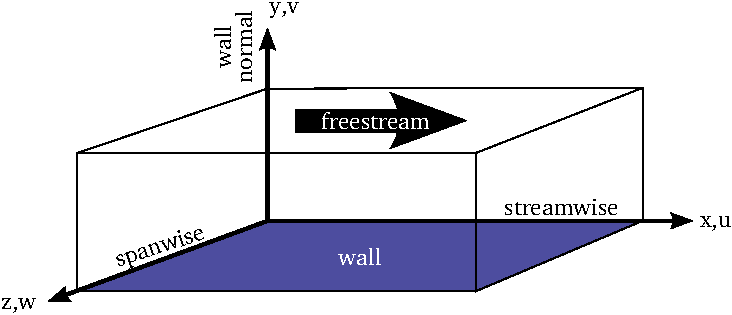
\includegraphics[width=.99\linewidth]{FlatPlateSchematic}
%%%      \end{center}
%%%    \end{column}
%%%    \begin{column}{0.41\linewidth}
%%%        Fixed freestream velocity drives mean streamwise flow\\
%%%        \vspace{\baselineskip}
%%%        Statistically two-dimensional
%%%    \end{column}
%%%  \end{columns}
%%%\end{block}
%%%\end{frame}

%===============================================================================
\begin{frame}{Spatially evolving boundary layer simulations are difficult}
\begin{center}
    %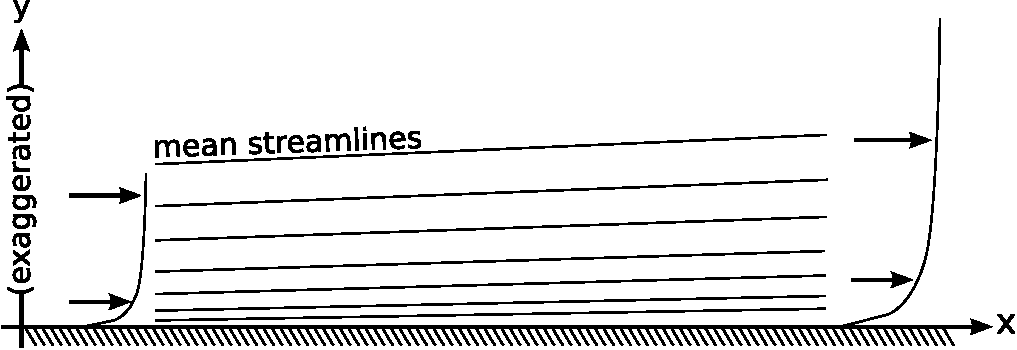
\includegraphics[width=0.65\textwidth]{Motivation1988Figure1a}
    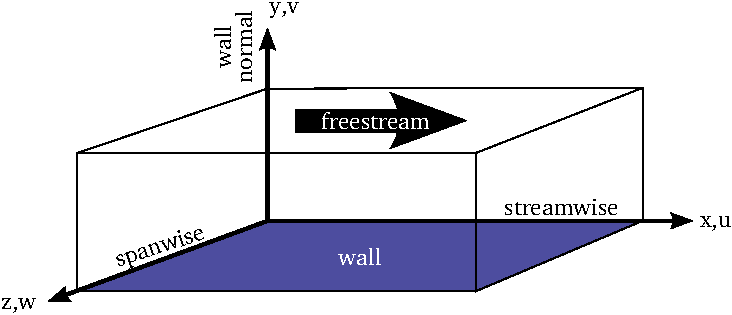
\includegraphics[width=.50\linewidth]{FlatPlateSchematic}
\end{center}
\vspace{-0.5em}
\begin{itemize}
  \item One must somehow specify inflow behavior:
    \begin{itemize}
      \item Tripping a laminar profile to force transition
            (e.g. \citet{Wu1999Simulation})
      \item Generate an approximately turbulent profile
            (e.g. \citet{Lund1998Generation})
      \item Recycle from elsewhere in the simulation
            (e.g. \citet{Simens2009Highresolution})
      \item Perform an auxiliary simulation to obtain an inflow profile
    \end{itemize}
  \item All choices require time before the profile ``relaxes'' to the right state
  \item \citet{Schlatter2010Assessment} assessed low-\Reynolds{}
        simulations\footnote{%
            \tiny
            \citet{Spalart1988Direct, Komminaho2002Reynolds, Khujadze2007New,
            Khujadze2004DNS, Ferrante2005Reynolds, Simens2009Highresolution,
            Wu2009Direct, Schlatter2009High, Schlatter2009Turbulent}
        }\\ finding ``\dots{}surprisingly inconsistent predictions\dots{}''
\end{itemize}
\end{frame}

%===============================================================================
\begin{frame}{Research Objective}
    Reduce turbulence-driven uncertainty by generating\\
    high-quality turbulent boundary layer calibration data for
    \begin{itemize}
        \item Cold wall
        \item Wall blowing
        \item Favorable pressure gradients
        \item<2-> \sout{Chemically reacting species under high-enthalpy conditions}
        \item<2-> \sout{Convex surface curvature}
        \item<2-> \sout{Surface roughness}
    \end{itemize}
\end{frame}

%===============================================================================
\subsection{Formulation and Numerics}
%===============================================================================

%===============================================================================
\begin{frame}{Homogenized boundary layer simulations are less difficult}
\vspace{1em}
\begin{columns}[c,onlytextwidth]
  \begin{column}{0.50\linewidth}
    \centering
    \only<1->{%
        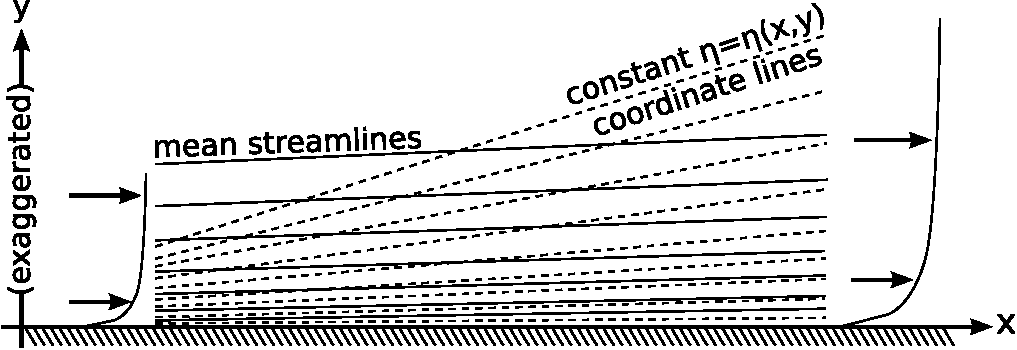
\includegraphics[width=0.99\textwidth]{Spalart1988Figure1a}
    }
  \end{column}
  \begin{column}{0.23\linewidth}
    \centering
    \only<2->{%
        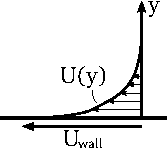
\includegraphics[width=0.82\linewidth]{rayleigh_cartoon}
    }
  \end{column}
  \begin{column}{0.20\linewidth}
    \centering
    \only<3->{%
        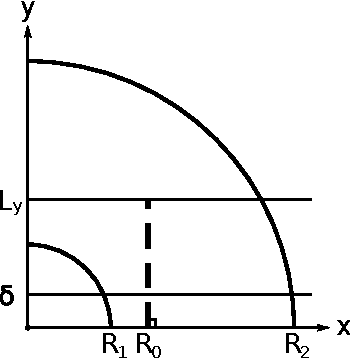
\includegraphics[width=0.82\linewidth]{nozzle_schematic}
    }
  \end{column}
\end{columns}
\begin{itemize}
  \item<1-> \citet{Spalart1988Direct} observed layer thickness and energy
        vary slowly in $x$
        \begin{itemize}
          \item Separated ``slow'' and ``fast'' spatial evolution
          \item Fast evolution assumed periodic---
                no need to specify inflow behavior
          \item Modeled impact of resulting ``slow growth'' terms on a
                ``fast'' simulation
          \item \citet{Guarini1998} extended technique to
                compressible case
        \end{itemize}
  \item<1-> Two periodic directions entirely sidesteps subtle inflow conditions\\
        $\implies$ spectral techniques, smaller sampling error
        $\implies$ reduced uncertainty
  \item<1-> Spatial homogenization not suited to calibrating off-the-shelf models
  \item<2-> \citet{Topalian2011Slow} temporally homogenized Rayleigh's problem
    %\begin{itemize}
    % \item Separates slow and fast temporal evolution,
    %       permitting use in calibration
    % \item Ongoing work to add homogenization with pressure gradients
    %\end{itemize}
  \item<3-> \citet{Topalian2014Spatiotemporal} spatiotemporal extension\\
        adds ``inviscid base flow'' terms permitting pressure gradients
\end{itemize}
\end{frame}


%===============================================================================
\begin{frame}{Compressible Navier--Stokes formulation}
\begin{footnotesize}
\label{eq:nondim_model}
\begin{align}
  \label{eq:nondim_continuity}
  \frac{\partial}{\partial{}t}\rho{}
 =
 &- \nabla\cdot\rho{}u
  + {\color{red}\Ssd_\rho}
  \\
  \label{eq:nondim_momentum}
  \frac{\partial}{\partial{}t}\rho{}u
 =
 &- \nabla\cdot(u\otimes\rho{}u)
  - \frac{1}{\Mach^{2}} \nabla{} p
  + \frac{1}{\Reynolds} \nabla\cdot\tau
  + f
  + {\color{red}\Ssd_{\rho{}u}}
  \\
  \label{eq:nondim_energy}
  \frac{\partial}{\partial{}t} \rho{}E
 =
 &- \nabla\cdot\rho{}Eu
  + \frac{1}{\Reynolds\,\Prandtl\,\left( \gamma - 1 \right)}
    \nabla\cdot\mu\nabla{} T
\\
 &- \nabla\cdot{} p u
  + \frac{\Mach^{2}}{\Reynolds} \nabla\cdot\tau{} u
  + \Mach^{2} f \cdot{} u
  + q_{b}
  + {\color{red}\Ssd_{\rho{}E}}
\end{align}
\vfill
\begin{align}
  p &= \left(\gamma-1\right) \left(
    \rho{}E - \frac{\Mach^{2}}{2}\rho{}u^{2}
  \right)
  &
  T &= \gamma{} \frac{p}{\rho}
\end{align}
\begin{align}
  \mu &= T^{\beta}
  &
  \lambda &= \left(\alpha-\frac{2}{3}\right)\mu
  &
  \tau &=  \mu\left(\nabla{}u+\trans{\nabla{}u}\right)
         + \lambda\left(\nabla\cdot{}u\right) I
\end{align}
\begin{align}
  \Reynolds &= \frac{\rho_0 u_0 l_0}{\mu_0}
&
  \Mach &= \frac{u_0}{a_0}
&
  \Prandtl &= \frac{\mu_0 C_p}{\kappa_0}
&
  \Knudsen &= \frac{\Mach}{\Reynolds}\sqrt{\frac{\gamma\pi}{2}}
\end{align}
\end{footnotesize}
\end{frame}

%%%%===============================================================================
%%%\begin{frame}{Modeling assumptions underneath the formulation}
%%%\begin{columns}[c]
%%%  \begin{column}{.45\textwidth}
%%%    \begin{enumerate}
%%%      \item Ideal gas with constant $\gamma$
%%%      \item Newtonian fluid obeying Stokes' hypothesis
%%%        \begin{itemize}
%%%          \item Isotropic viscous stress tensor depending
%%%                linearly on $\vec{\nabla}\vec{u}
%%%                +\trans{\vec{\nabla}\vec{u}}$
%%%          \item Bulk and dynamic viscosities related by
%%%                $\mu_B = \alpha\mu$
%%%        \end{itemize}
%%%      \item Power law viscosity: $\mu/\mu_0 = \left( T/T_0 \right)^\beta$
%%%      \item Fourier's law: $q=-\kappa\nabla{}T$
%%%      \item Constant Prandtl number $\implies \mu/\mu_0 = \kappa/\kappa_0$
%%%    \end{enumerate}
%%%  \end{column}
%%%  \begin{column}{.55\textwidth}
%%%    \nocite{NASA-TR-R-132}
%%%    \includegraphics[width=0.95\textwidth,clip=true,trim=1.5in 0 2in 0]% Cont.
%%%        {AirViscosityVsTemperature}
%%%  \end{column}
%%%\end{columns}
%%%\end{frame}
%%%
%%%%===============================================================================
%%%\begin{frame}{Method of weighted residuals formalism\dots}
%%%\vfill
%%%\begin{block}{}
%%%Approximate
%%%$\frac{\partial}{\partial{}t} u = \mathscr{N}\!\left(u\right)$
%%%by
%%%$\frac{\partial}{\partial{}t} u^h = \mathscr{N}\!\left(u^h\right)+R^h$.
%%%\\
%%%\vspace{0.75em}
%%%Choose $L_2$ inner product on
%%%$\left[-\frac{L_x}{2},\frac{L_x}{2}\right] \times{}
%%%[0,L_y] \times{} \left[-\frac{L_z}{2},\frac{L_z}{2}\right]$.
%%%\\
%%%\vspace{0.75em}
%%%Expand
%%%\begin{align}
%%%  u^h(x,y,z,t)
%%%  &=
%%%    \sum_{l=0}^{N_y - 1}
%%%    \sum_{m=-\frac{N_x}{2}}^{\frac{N_x}{2}-1}
%%%    \sum_{n=-\frac{N_z}{2}}^{\frac{N_z}{2}-1}
%%%    \hat{u}_{l,m,n}(t)
%%%    B_l\!\left(y\right)
%%%    e^{\ii\frac{2\pi{}m}{L_x}x}
%%%    e^{\ii\frac{2\pi{}n}{L_z}z}
%%%    \\
%%%  &=
%%%    \sum_{l}\sum_{m}\sum_{n}
%%%    \hat{u}_{l,m,n}(t)B_l\!\left(y\right)e^{\ii k_m x}e^{\ii k_n z}
%%%\end{align}
%%%where
%%%$k_m = 2\pi{}m/L_x$, $k_n = 2\pi{}n/L_z$, and $B_l\!\left(y\right)$
%%%are a B-spline basis.
%%%\\
%%%\vspace{0.75em}
%%%Test with ``functions'' like
%%%$\delta(y-y_{l'}) e^{\ii k_{m'} x}e^{\ii k_{n'} z}$
%%%and set residual to zero.
%%%\end{block}
%%%\end{frame}
%%%
%%%%===============================================================================
%%%\begin{frame}{\dots{}leads to a pseudospectral technique}
%%%\begin{block}{}
%%%Push through simple algebra to get
%%%{\tiny
%%%\begin{align}
%%%  L_x L_z
%%%  &\sum_{l} B_l\!\left(y_{l'}\right)
%%%  \frac{\partial}{\partial{}t} \hat{u}_{l,m,n}(t)
%%%  =
%%%  \\
%%%  &\int_{-\frac{L_x}{2}}^{\frac{L_x}{2}}
%%%  \int_{-\frac{L_z}{2}}^{\frac{L_z}{2}}
%%%  \mathscr{N}\left(
%%%    \sum_{m}\sum_{n}
%%%    \left(
%%%      \sum_{l} B_l\!\left(y_{l'}\right)
%%%      \hat{u}_{l,m,n}(t)
%%%    \right)
%%%    e^{\ii k_m x}e^{\ii k_n z}
%%%  \right)
%%%  \left(
%%%    e^{-\ii k_{m'} x}e^{-\ii k_{n'} z}
%%%  \right)
%%%  \, dz \, dx
%%%  .
%%%\end{align}
%%%}
%%%\\
%%%Finally, approximate integrals using
%%%{\tiny
%%%\begin{align}
%%%  \sum_{l}
%%%  B_l\!&\left(y_{l'}\right)
%%%  \frac{\partial}{\partial{}t} \hat{u}_{l,m,n}(t)
%%%  \approx
%%%\\
%%%  &\frac{1}{N_x N_z}
%%%  \sum_{m'} \sum_{n'}
%%%  \mathscr{N}\left(
%%%    \sum_{m}
%%%    \sum_{n}
%%%    \left(
%%%      \sum_{l} B_l\!\left(y_{l'}\right)
%%%      \hat{u}_{l,m,n}(t)
%%%    \right)
%%%    e^{\ii k_m x_{m'}}e^{\ii k_n z_{n'}}
%%%  \right)
%%%  \left(
%%%    e^{-\ii k_{m'} x_m}e^{-\ii k_{n'} z_n}
%%%  \right)
%%%  .
%%%\end{align}
%%%}
%%%\\
%%%\end{block}
%%%\begin{center}
%%%  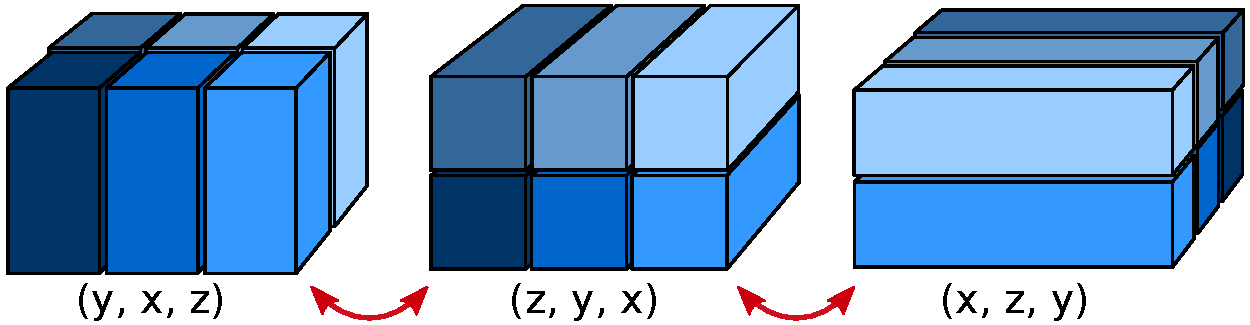
\includegraphics[width=.7\linewidth]{PencilTransposeSchematic}
%%%\end{center}
%%%\end{frame}
%%%
%%%
%%%%===============================================================================
%%%\begin{frame}{Time discretization}
%%%\begin{block}{Low storage, hybrid implicit/explicit SMR91 scheme}
%%%  \begin{itemize}
%%%   \item Want statistics over long times, but CFLs quite restrictive
%%%   \item Implicit nonlinear solves infeasible;\\
%%%         Split $\mathscr{N}\!\left(u\right)$ into
%%%         $M^{-1}Lu + \chi{}M^{-1}N\!\left(u\right)$
%%%  \end{itemize}
%%%\end{block}
%%%\begin{block}{Scheme from \citet*{spalart_lowstoragerk}}
%%%  \begin{columns}[C]
%%%    \begin{column}{0.40\linewidth}
%%%      Each substep governed by
%%%      {\tiny
%%%      \begin{align}
%%%        \left(M - \Delta{}t\beta_{i}L\right) u^{i+1}
%%%        &=
%%%        \left(M + \Delta{}t\alpha_{i}L\right) u^{i}
%%%        \\
%%%        {}&+ \Delta{}t\gamma_{i}\chi{}N\left(u^{i}\right)
%%%        \\
%%%        {}&+ \Delta{}t\zeta_{i-1}\chi{}N\left(u^{i-1}\right)
%%%      \end{align}
%%%      }
%%%    \end{column}
%%%    \begin{column}{0.58\linewidth}
%%%      {\tiny
%%%      \begin{algorithmic}
%%%        \REQUIRE Storage $a = u\left(t\right) = u^{0} $;
%%%                 storage $b$'s contents undefined
%%%        \STATE $b\leftarrow{}a$
%%%        \STATE $b\leftarrow{}N\left(b, t_n\right)$
%%%        \STATE Compute $\Delta{}t$ from $a=u^0$ and $b=N\left(u^0, t_n\right)$
%%%        \STATE $a\leftarrow{}\left(M+\Delta{}t\alpha_{1}L\right)a$
%%%        \STATE $a\leftarrow{}\Delta{}t \gamma_{1} \chi{} b + a$
%%%        \STATE $a\leftarrow{}\left(M-\Delta{}t\beta_{1}L\right)^{-1}a$
%%%        \ENSURE Storage $a = u^1$;
%%%                storage $b = N\left(u^{0},t_n\right)$
%%%        \STATE $b\leftarrow{}\left(M+\Delta{}t\alpha_{2}L\right)a
%%%                            +\Delta{}t\zeta_{1}\chi{}b$
%%%        \STATE $a\leftrightarrow{}b$
%%%        \STATE $b\leftarrow{}N\left(b,t_n+\eta_2\Delta{}t\right)$
%%%        \STATE $a\leftarrow{}\Delta{}t \gamma_{2} \chi{} b + a$
%%%        \STATE $a\leftarrow{}\left(M-\Delta{}t\beta_{2}L\right)^{-1}a$
%%%        \ENSURE Storage $a = u^{2}$;
%%%                storage $b = N\left(u^{1}, t_n + \eta_2\Delta{}t\right)$
%%%        \STATE $\dots$
%%%%         \STATE $b\leftarrow{}\Delta{}t\zeta_{2}b$
%%%%         \STATE $b\leftarrow{}b+\left(M+\Delta{}t\alpha_{3}L\right)a$
%%%%         \STATE $a\leftrightarrow{}b$
%%%%         \STATE $b\leftarrow{}N\left(b\right)$
%%%%         \STATE $a\leftarrow{}a + \Delta{}t \gamma_{3} b$
%%%%         \STATE $a\leftarrow{}\left(M-\Delta{}t\beta_{3}L\right)^{-1}a$
%%%%         \ENSURE Storage $a = u\left(t+\Delta{}t\right)= u^{3}$;
%%%%                 storage $b = N\left(u^{2}\right)$
%%%      \end{algorithmic}
%%%      }
%%%    \end{column}
%%%  \end{columns}
%%%\end{block}
%%%\end{frame}
%%%
%%%%===============================================================================
%%%\subsection{Implementation: Suzerain}
%%%%===============================================================================

%===============================================================================
\begin{frame}
\frametitle{Suzerain: a new spectral, compressible DNS framework}
\framesubtitle{\texttt{http://github.com/RhysU/suzerain}}
\vspace{-1.5em}
\begin{columns}[t]
\begin{column}{.50\textwidth}
\begin{small}
\begin{itemize}
  \item ``Clean room'' C99/C++03 implementation
        built as long-lived, extensible research platform
  \item Fourier--Galerkin, B-spline collocation spatial scheme
  \item Hybrid implicit/explicit,\\low-storage temporal scheme\\
        \citep{spalart_lowstoragerk}
  \item Automated test suite and MMS-based verification\\
        \citep{Ulerich2012MMS}
  \item \emph{In situ} statistics collection\\and post-processing
  \item Autoregressive-based uncertainty estimation per~\citet{Oliver2014Estimating}
\end{itemize}
\end{small}
\end{column}
\begin{column}{.50\textwidth}
  \vspace{-1em}
  \begin{center}
    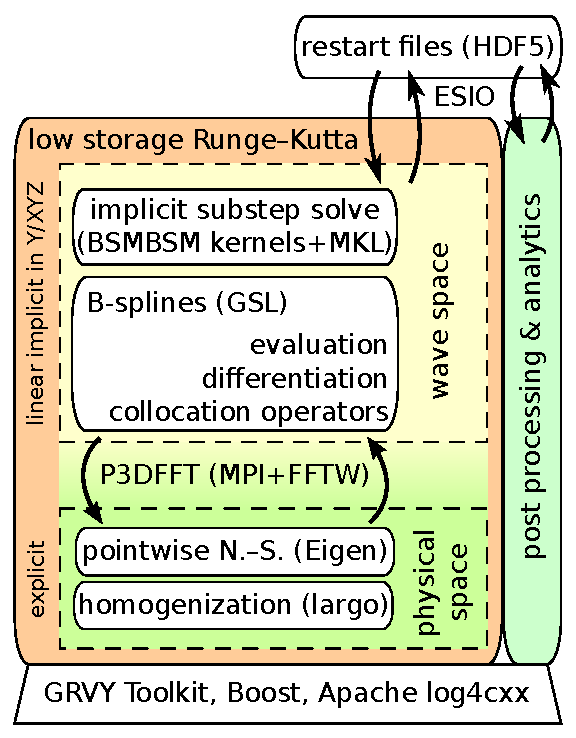
\includegraphics[width=0.95\textwidth]{SuzerainDesignOverview}
  \end{center}
\end{column}
\end{columns}
\end{frame}

%%%%===============================================================================
%%%\begin{frame}{Testing and MMS-based Verification}
%%%%
%%%\begin{block}{}
%%%32K SLOC, 27K Tests with 80\% line coverage, 10K Model Documentation
%%%\end{block}
%%%%
%%%\begin{figure}
%%%\centering
%%%\vspace{-0.75em}
%%%\includegraphics[width=0.99\textwidth]{mms-convergence}
%%%\caption{\scriptsize
%%%  Field-by-field convergence for Suzerain on a steady (left) and
%%%  transient (right) problem at two different B-spline orders.  Labels $Q_\rho$
%%%  and $Q_{\rho{}u}$ show measured relative error in the associated floating point
%%%  manufactured forcing computations.  Label $\epsilon$ shows machine epsilon.
%%%  \citet{Ulerich2012MMS}
%%%}
%%%\end{figure}
%%%%
%%%\end{frame}
%%%
%%%%===============================================================================
%%%\begin{frame}{Scalability Results}
%%%             {Pessimistic largest conceivable problem size of interest}
%%%  \begin{figure}[h]
%%%    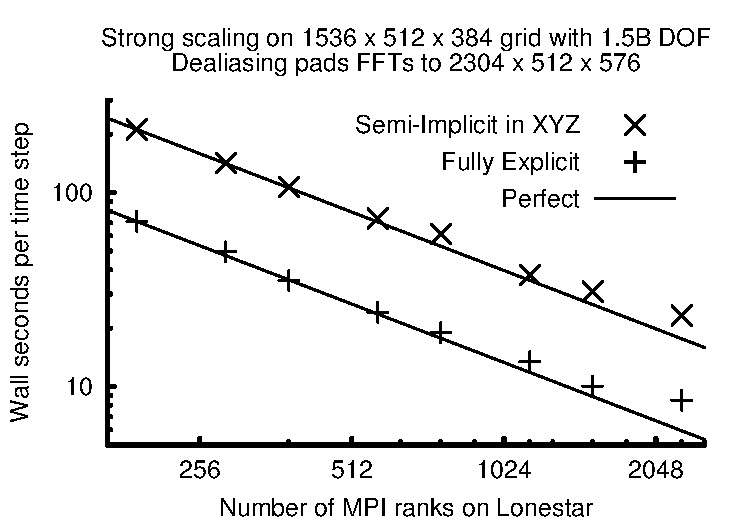
\includegraphics[width=0.85\textwidth]{scaling_upper}
%%%  \end{figure}
%%%\end{frame}
%%%
%%%%===============================================================================
%%%\begin{frame}{Scalability Results}
%%%             {Anticipated homogenized boundary layer grid,
%%%              $\Reynolds[\theta]{}=770$,
%%%              $\Mach[e]{}=1.2$}
%%%  \begin{figure}[h]
%%%    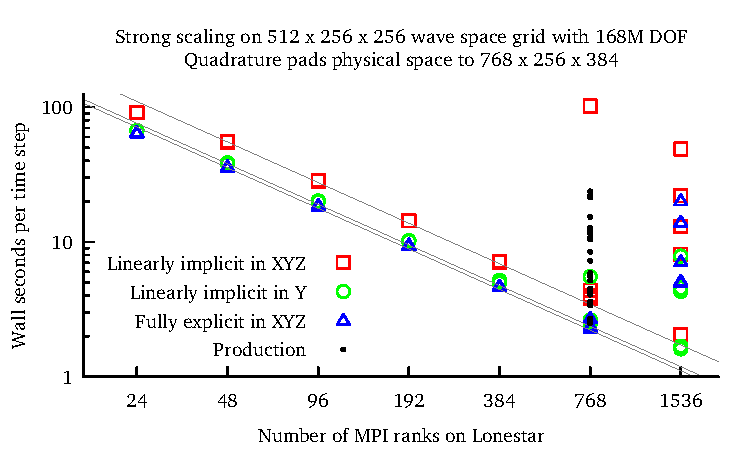
\includegraphics[width=0.85\textwidth]{scaling}
%%%  \end{figure}
%%%\end{frame}
%%%
%%%%===============================================================================
%%%\subsection{Results: Isothermal Channel Database}
%%%%===============================================================================
%%%
%%%%===============================================================================
%%%\begin{frame}{Scenarios patterned on \citet{Coleman1995Numerical}}
%%%\begin{center}
%%%  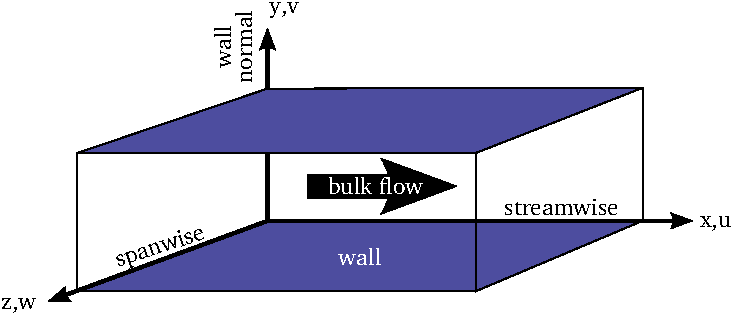
\includegraphics[width=0.85\linewidth]{ChannelSchematic}
%%%\end{center}
%%%\begin{align*}
%%%  u_w &= 0
%%%  &
%%%  T_w &= 1
%%%  &
%%%  f : \left(\rho{}u\right)_\text{bulk} &= 1
%%%  &
%%%  q_b &= 0
%%%  &
%%%  \rho_\text{bulk} &= 1
%%%\end{align*}
%%%\begin{align*}
%%%  \gamma &= 1.4
%%%  &
%%%  \Prandtl &= 2/3
%%%  &
%%%  \alpha &= 0
%%%  &
%%%  L &= 4\pi \times 2 \times 4\pi/3
%%%\end{align*}
%%%\begin{align*}
%%%  \Reynolds &= \left\{3000, 5000\right\}
%%%  &
%%%  \Mach &= \left\{ 0.1, 0.5, 1.5, 3.0 \right\}
%%%\end{align*}
%%%\end{frame}
%%%
%%%%===============================================================================
%%%\begin{frame}{Resolutions patterned on \citet{Coleman1995Numerical}}
%%%%
%%%\vfill
%%%%
%%%Fourier basis in $x$ and $z$ using 3/2s dealiasing: $N_x = 192$, $N_z = 168$\\
%%%Piecewise $7^\text{th}$ order B-splines in $y$ with hyperbolic tangent stretching\\
%%%%
%%%\begin{table}
%%%\centering
%%%\resizebox{\textwidth}{!}{
%%%\begin{tabular}{c|ccccc|cccc|c}
%%%Identifier                               & % Simulation input parameters
%%%$\textrm{Re}$                            &
%%%$\textrm{Ma}$                            &
%%%$\beta$                                  &
%%%$N_y$                                    &
%%%$\tanh$                                  &
%%%$\Delta{}x^{+}$                          & % Details from post-processing
%%%$\Delta{}y_{1}^{+}$                      &
%%%$\Delta{}y_{10}^{+}$                     &
%%%$\Delta{}z^{+}$                          &
%%%Flow throughs
%%%\\
%%%\hline \hline
%%%%id       &  Re    &  Ma   &  beta  &  Ny   &  tanh  & x+    &  y+1   &   y+10  &  z+    &   Flowthroughs  \\
%%%c03k01    &  3000  &  0.1  &  2/3   &  128  &  2.25  & 12.5  &  0.22  &   11.8  &  5.0   &   37.1          \\
%%%c03k05    &  3000  &  0.5  &  2/3   &  128  &  2.25  & 12.6  &  0.22  &   12.0  &  5.1   &   38.9          \\
%%%\rowcolor{yellow}
%%%c03k15    &  3000  &  1.5  &  2/3   &  128  &  2.25  & 14.4  &  0.25  &   13.7  &  5.8   &   39.1          \\
%%%c03k30    &  3000  &  3.0  &  2/3   &  128  &  2.25  & 19.5  &  0.34  &   18.5  &  7.8   &   38.8          \\
%%%\hline
%%%c05k01    &  5000  &  0.1  &  2/3   &  144  &  2.50  & 19.4  &  0.26  &   14.1  &  7.8   &   30.6          \\
%%%c05k05    &  5000  &  0.5  &  2/3   &  144  &  2.50  & 19.8  &  0.27  &   14.4  &  7.9   &   32.0          \\
%%%c05k15    &  5000  &  1.5  &  2/3   &  144  &  2.50  & 22.8  &  0.30  &   16.5  &  9.1   &   48.7          \\
%%%c05k30    &  5000  &  3.0  &  2/3   &  144  &  2.50  & 30.9  &  0.41  &   22.4  &  12.3  &   81.7          \\
%%%\hline
%%%\rowcolor{yellow}
%%%CKM95a    &  3000  &  1.5  &  0.7   &   90  &        &   17  &   0.1  &     8   &  10    &  $\geq 11.9$    \\
%%%CKM95b    &  4880  &  3.0  &  0.7   &   90  &        &   39  &   0.2  &     17  &  24    &  $\geq 11.9$
%%%\end{tabular}
%%%}%resizebox
%%%\end{table}
%%%%
%%%\vfill
%%%%
%%%CKM95\{a,b\} by \citet{Coleman1995Numerical} used Fourier--Legendre basis:\\
%%%$110 \times 90 \times 60$ coefficients with $144 \times 119 \times 80$ collocation points
%%%\end{frame}
%%%
%%%%===============================================================================
%%%\begin{frame}{Comparison w/ \citeauthor{Coleman1995Numerical}
%%%              for $\Reynolds=3000$, $\Mach=1.5$}
%%%\vspace{1em}
%%%\begin{columns}[t]
%%%  \begin{column}{.50\linewidth}
%%%    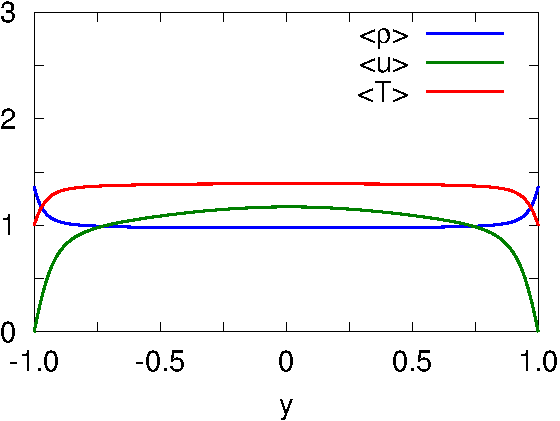
\includegraphics[width=0.99\linewidth]{c03k15_figure7a}
%%%  \end{column}
%%%  \begin{column}{.50\linewidth}
%%%    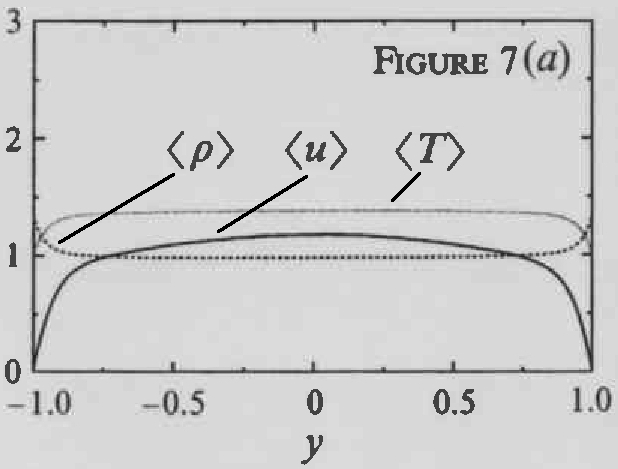
\includegraphics[width=0.99\linewidth]{ckm95_figure7a}
%%%  \end{column}
%%%\end{columns}
%%%\vfill
%%%\begin{table}
%%%\centering
%%%\resizebox{\textwidth}{!}{
%%%\begin{tabular}{c|ccccc|cccc}
%%%Identifier                               &
%%%$\textrm{Ma}_c$                          &
%%%$\textrm{Ma}_\tau$                       &
%%%$\textrm{Re}_c$                          &
%%%$\textrm{Re}_\tau$                       &
%%%$-\textrm{B}_q$                          &
%%%$\left<\rho_w\right>$                    &
%%%$\left<\rho_c\right>$                    &
%%%$\left<T_c\right>$                       &
%%%$\left<\mu_c\right>$
%%%\\
%%%\hline \hline
%%%%id     &  Mac    &  Matau  &  Rec   &  Retau  &  -Bq     &  rhow   &  rhoc    &  Tc     &  muc    \\
%%%c03k15  &  1.493  &  0.081  &  2765  &  221    &  0.049   &  1.365  &  0.978   &  1.391  &  1.246  \\
%%%CKM95a  &  1.502  &  0.082  &  2760  &  222    &  0.049   &  1.355  &  0.980   &  1.378  &  1.252  \\
%%%\end{tabular}
%%%}%resizebox
%%%\end{table}
%%%\vspace{0.25em}
%%%\begin{footnotesize}\begin{flushright}
%%%Tabulated discrepancies between c03k15 and
%%%CKM95a less than $1\%$, except $\Mach[\tau]\leq{}1.5\%$
%%%\end{flushright}\end{footnotesize}
%%%\end{frame}
%%%
%%%%===============================================================================
%%%\begin{frame}{Statistics with precisely quantified uncertainty: c03k15}
%%%\begin{center}
%%%\vfill
%%%\includegraphics[width=0.99\textwidth]{basic3k15}
%%%\end{center}
%%%\end{frame}
%%%

%===============================================================================
\subsection{Scenario of Interest and New Simulations}
%===============================================================================

\begin{frame}
\frametitle{Fully turbulent Orion MPCV from \citet{Bauman2011Loose}}
\framesubtitle{Translated to $\gamma=1.4$ air holding $\Mach[e]{}$ constant.  Reduction by O. Sahni \& V. Topalian.}
\begin{columns}
  \begin{column}{0.40\textwidth}
    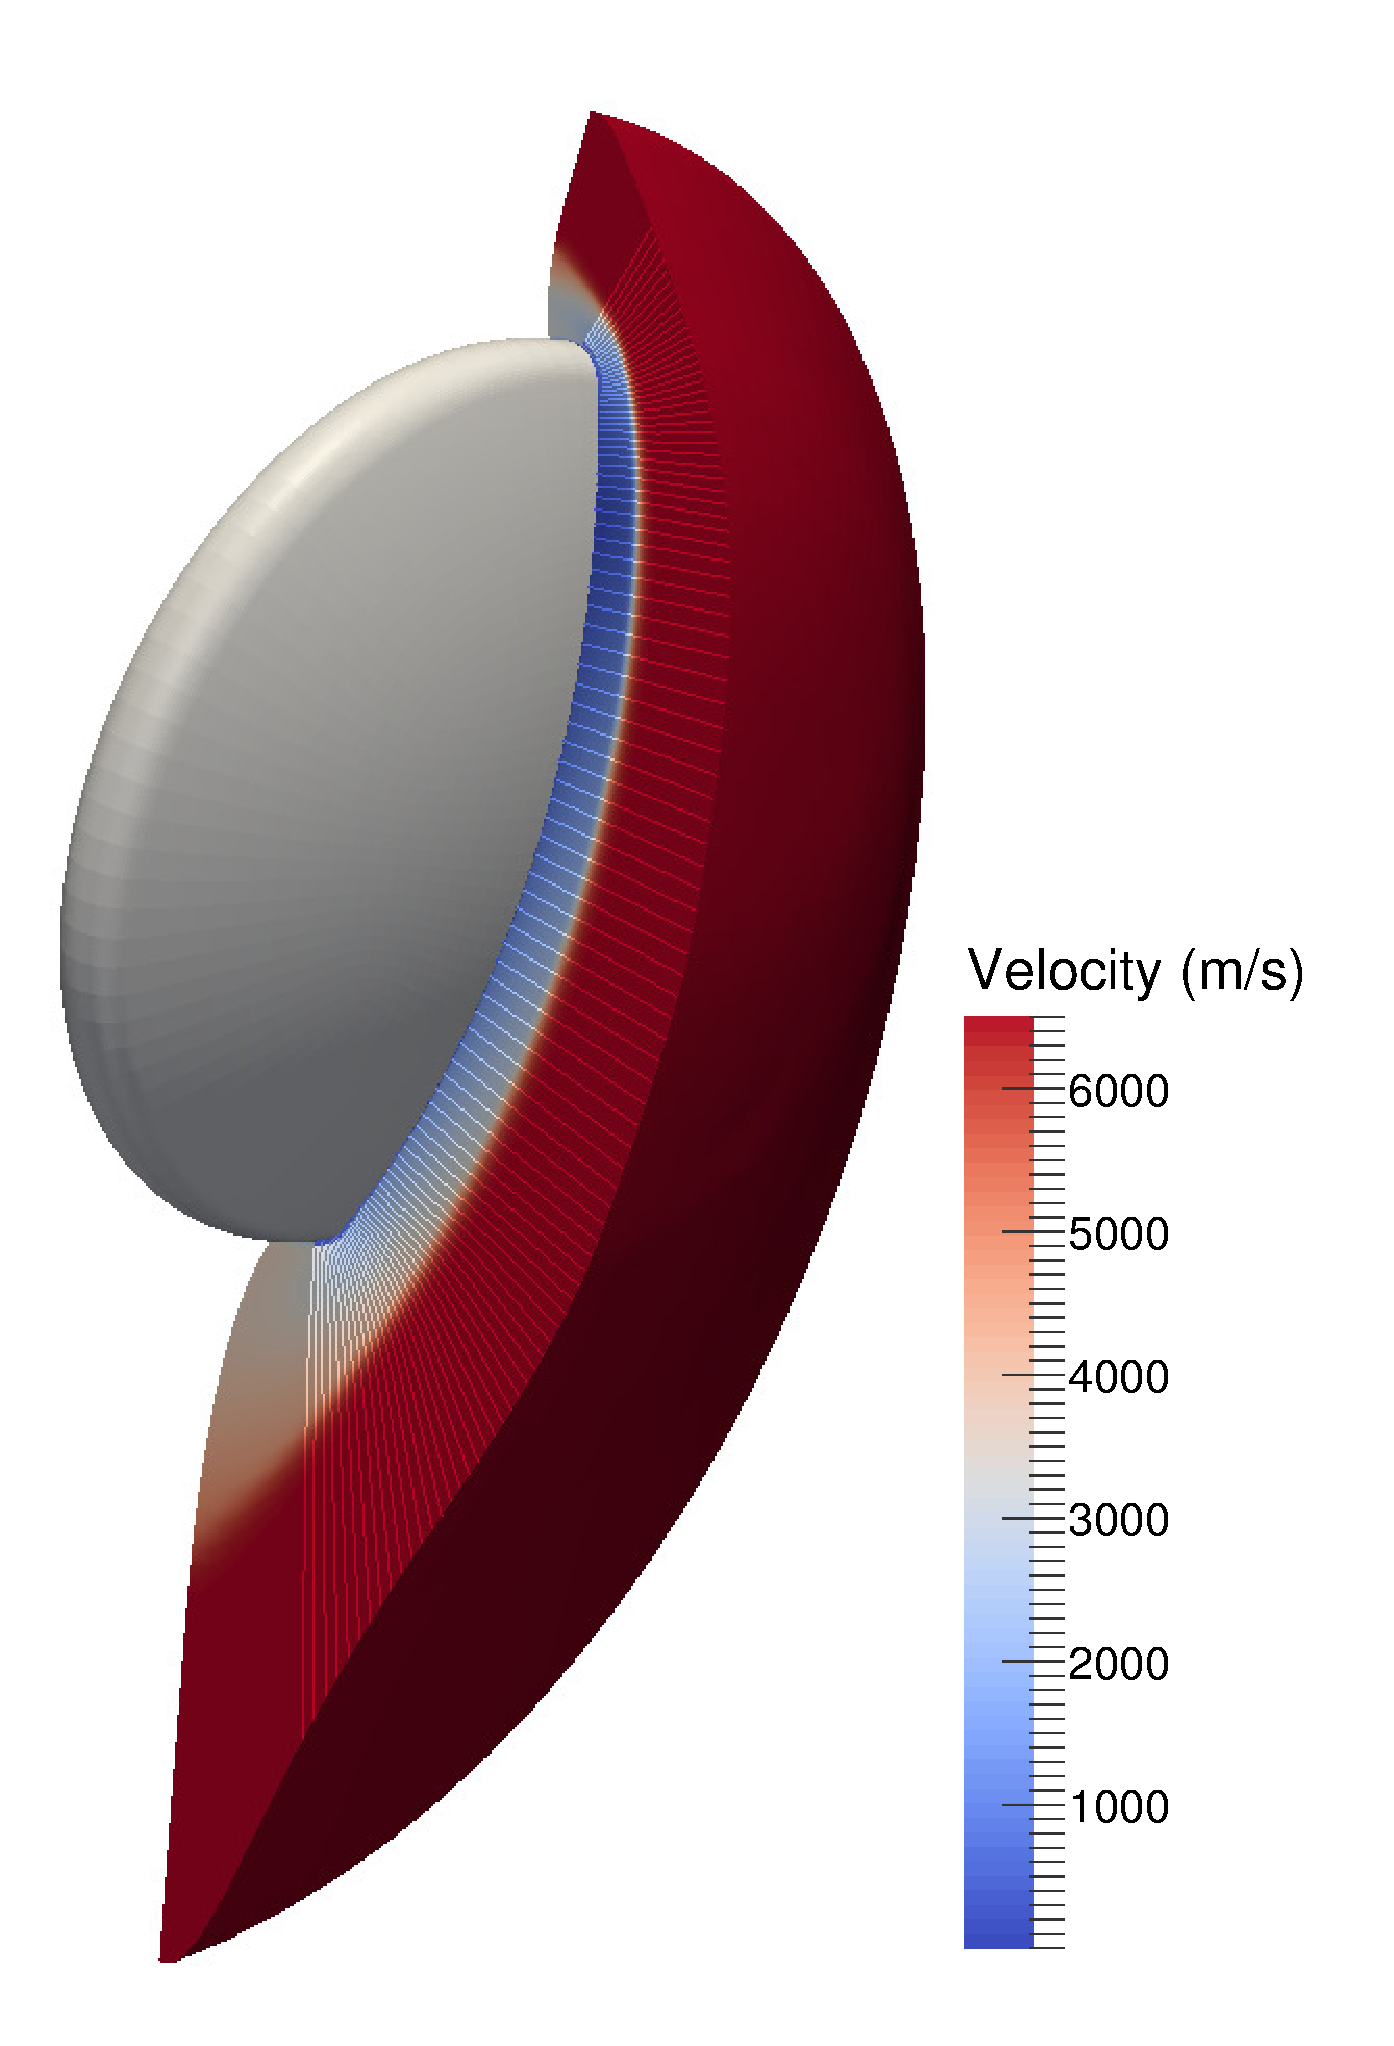
\includegraphics[width=0.90\textwidth]{symplanenorm}
  \end{column}
  \begin{column}{0.50\textwidth}
%%% BEGIN table_cevissturb.tex
\begin{tabular}{ccc}
{$\Reynolds[\theta]{}=\frac{\rho_e{}u_e{}\theta}{\mu_e}$} &
{$\Mach[e]{} = \frac{u_e}{a_e}$}  &
{$\beta=\frac{\delta^\ast}{\tau_w}\left(\frac{\partial{}p}{\partial\xi}\right)_e$}  \\
\hline
391  &  0.88  &  -0.81  \\
440  &  0.99  &  -0.81  \\
511  &  1.09  &  -0.93  \\
520  &  1.15  &  -0.92  \\
526  &  1.19  &  -0.94
\end{tabular}
%%% END table_cevissturb.tex
  \end{column}
  \begin{column}{0.08\textwidth}
      % EMPTY
  \end{column}
\end{columns}
\end{frame}

\begin{frame}
    \frametitle{Fully laminar\\Orion MPCV}
    \framesubtitle{Data courtesy of P. Bauman\\Reduction in present work}
    \vspace{-6.25em}
    \begin{flushright}
        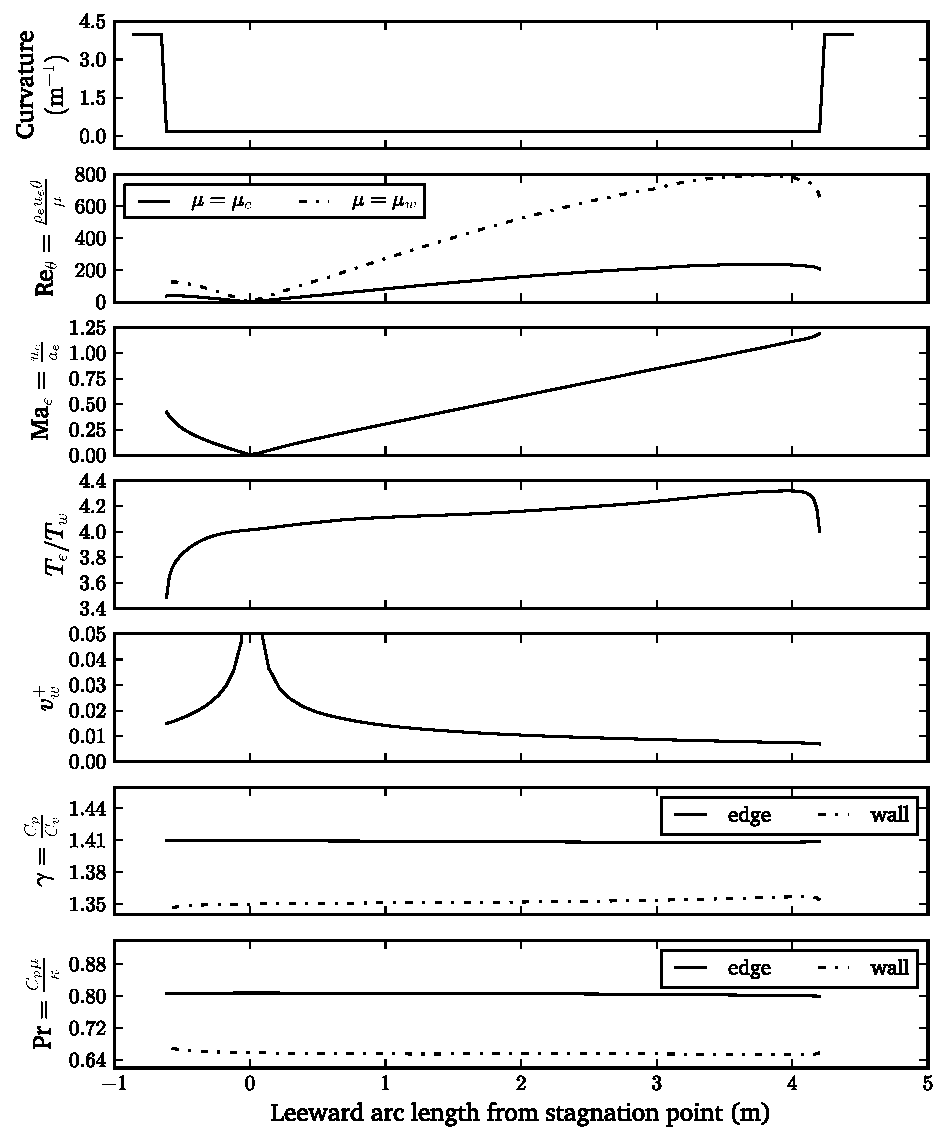
\includegraphics[height=0.99\textheight]{cevisslam_summary1}
    \end{flushright}
\end{frame}

\begin{frame}
\frametitle{New Direct Numerical Simulations}
\framesubtitle{%
    Domain is $10\delta \times 2.5\delta \times 3\delta$
    with $512 \times 256 \times 256$ expansion coefficients for 168M DOF
}
\centering
% BEGIN table_turb_hbl.tex
\begin{tabular}{lcccccccccc}
\multicolumn{1}{c}{\raisebox{0.75ex}{Case}}                  &
\raisebox{0.75ex}{$\textrm{Re}_{\theta}$}                    &
\raisebox{0.75ex}{$\textrm{Ma}_{99}$}                        &
\raisebox{0.75ex}{$T_{99}/T_w$}                              &
\raisebox{0.75ex}{$v_w^{+}=v_w/u_\tau$}                      &
\raisebox{0.75ex}{$p_{{99},\xi}^{\ast}=\frac{\delta_{99} \left(\partial_x p\right)_{99}}{\rho_{99} u_{99}^2}$}
\\
\toprule
%Case   &  Re_theta  &  Ma_99  &  ratio_T  &  vwallplus      &  p_ex          \\
 t3.199 &  382       &  0.904  &  4.13     &  \num{8.52e-3}  &  \num{-0.010}  \\
 t4.134 &  531       &  1.152  &  4.20     &  \num{7.18e-3}  &  \num{-0.012}
\end{tabular}
%
\\\vfill
%
\begin{tabular}{lccccccccccc}
\multicolumn{1}{c}{Case}         &
$\Delta{}x^{+}$                  &  %  Details  from  post-processing
$y_{1}^{+}$                      &
$y_{10}^{+}$                     &
$\Delta{}z^{+}$                  &
\shortstack[c]{Eddy\\Turnovers}
\\
\toprule
%Case                         &  x+    &  y+1    &  y+10   &  z+     &  Turnovers  \\
t3.199                        &  13.9  &  0.14   &  6.1    &  \z8.4  &  6.4      \\
t4.134                        &  19.0  &  0.17   &  7.2    &  11.4   &  6.9      \\
\citet{Coleman1995Numerical}  &  17\Z  &  0.1\z  &  8\Z    &  10\Z   &  ---
\end{tabular}
% END table_turb_hbl.tex
\end{frame}

\begin{frame}
    \frametitle{Resolution assessment for simulation t3.199}
    \framesubtitle{Compares favorably with \citet{Coleman1995Numerical} and \citet{Guarini2000Direct}}
    \begin{columns}
        \begin{column}{0.5\linewidth}
          \centering
          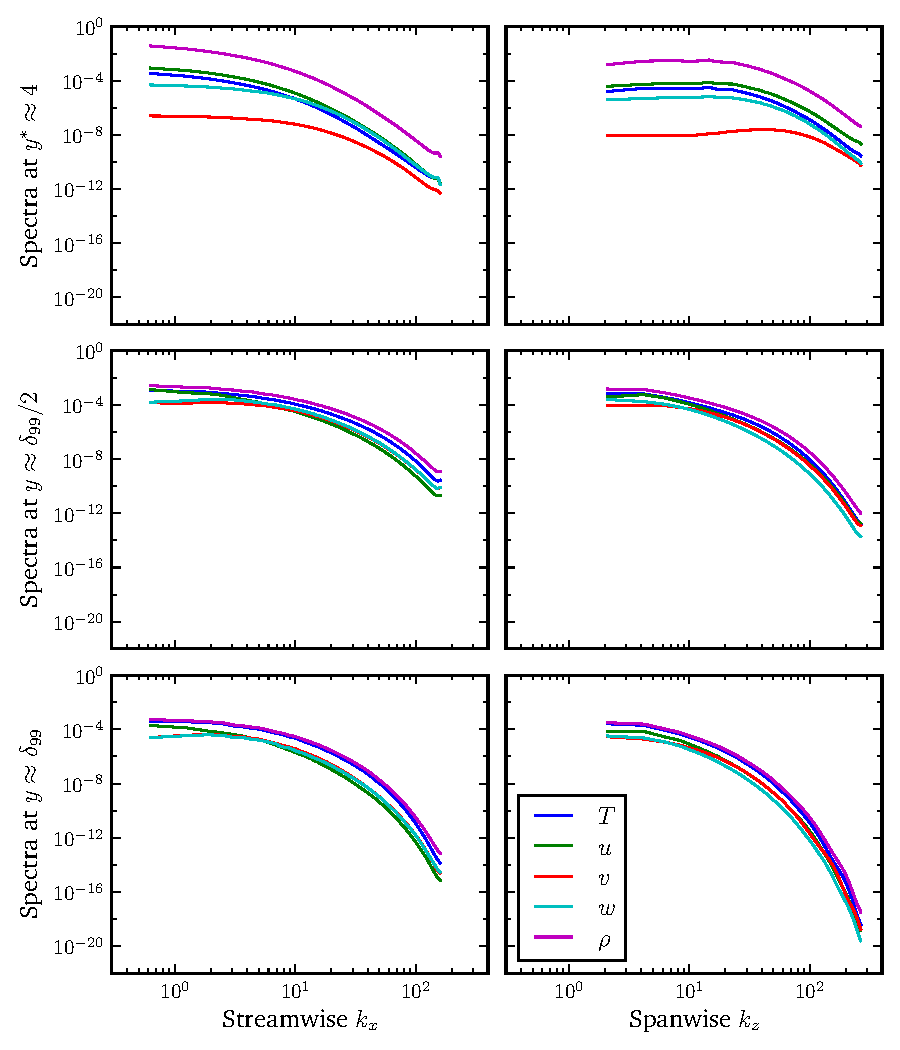
\includegraphics[width=\textwidth]{spectra-turb4134}
          \\\vspace{-0.5em}
          Spectra
        \end{column}
        \begin{column}{0.5\linewidth}
          \centering
          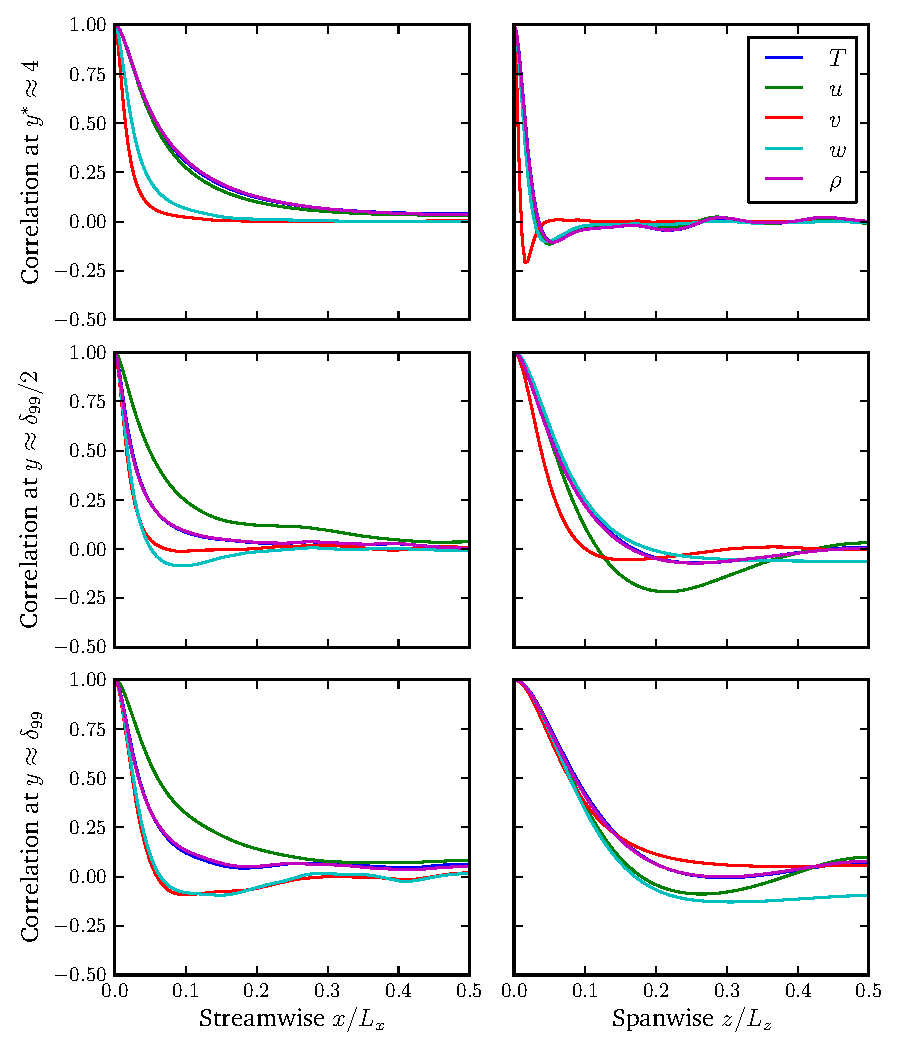
\includegraphics[width=\textwidth]{autocorr-turb4134}
          \\\vspace{-0.5em}
          Two-point correlations
        \end{column}
    \end{columns}
\end{frame}

% The nondimensional quantities are the Clauser parameter
% $\beta$~\citep{Clauser1954Turbulent}, Launder's acceleration parameter
% $K$~\citep{Launder1964Laminarization}, the Pohlhausen parameter~$K_s$,
% similarity parameter $\Lambda$~\citep{Cal2008Similarity}, parameter
% $\Lambda_n$~\citep{Narasimha1979Relaminarization}, and a new
% invention~$p_{e,\xi}^{\ast}$.
\begin{frame}
    \frametitle{Fully laminar\\Orion MPCV}
    \framesubtitle{Pressure gradient characterization}
    \vspace{-4.5em}
    \begin{columns}[c]
        \begin{column}{0.40\linewidth}
            \vspace{2em}
            \begin{description}
                \item[$\beta$]            \citet{Clauser1954Turbulent}
                \item[$K$]                \citet{Launder1964Laminarization}
                \item[$K_s$]              \citet{Pohlhausen1921Zur}
                \item[$\Lambda$]          \citet{Cal2008Similarity}
                \item[$\Lambda_n$]        \citet{Narasimha1979Relaminarization}
                \item[$p_{e,\xi}^{\ast}$] New parameter\\
                                          in present work
            \end{description}
        \end{column}
        \begin{column}{0.5\linewidth}
            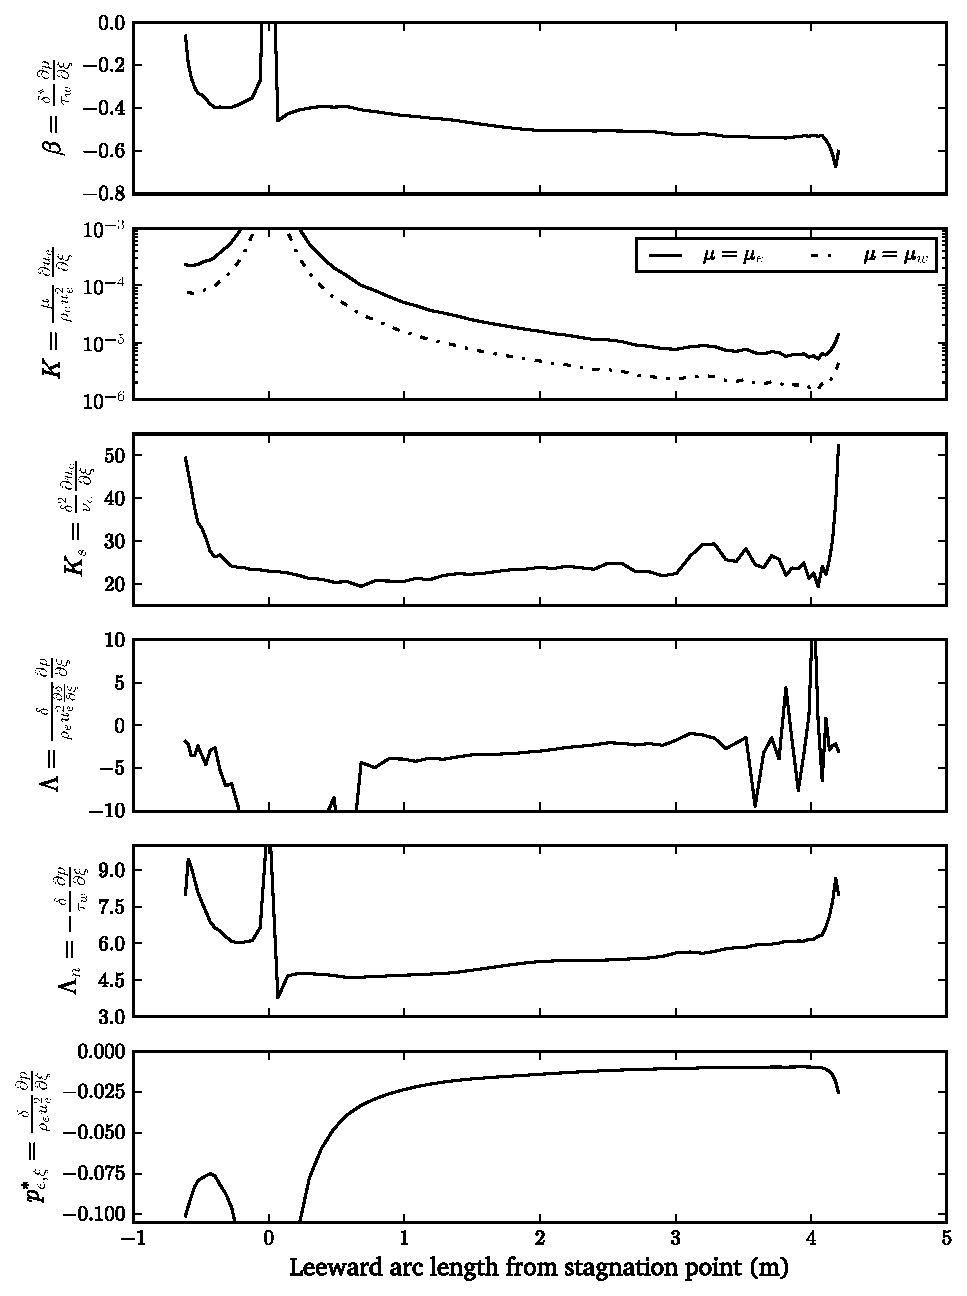
\includegraphics[height=0.99\textheight]{cevisslam_summary_fpg}
        \end{column}
    \end{columns}
\end{frame}

%%%%===============================================================================
%%%\begin{frame}{Proposed: Supersonic boundary layer database}
%%%             {High-quality calibration data for cold, transpiring walls
%%%              and favorable pressure gradients}
%%%\small
%%%\vspace{1em}
%%%\begin{table}
%%%\centering
%%%\begin{tabular}{l|rrrrr}
%%%Location number & 1 & 2 & 3 & 4 & 5 \\
%%%\hline
%%%\hline
%%% $T_e/T_w$                                                          & 3.514     & 3.486     & 3.464     & 3.452     & 3.430     \\
%%% $\beta = \frac{\delta^*}{\tau_w} \left|\frac{d p}{d \xi}\right|_e$ & 0.59      & 0.60      & 0.69      & 0.68      & 0.70      \\
%%% \hline
%%% $\beta$      (air, same $U$)                                       & 0.62      & 0.62      & 0.72      & 0.72      & 0.73      \\
%%% $\Mach[e]{}$                                                       & 1.14      & 1.28      & 1.41      & 1.48      & 1.53      \\
%%% $\Reynolds[\theta]{}$                                              & 506       & 568       & 658       & 668       & 676       \\
%%% $\tau_w$                                                           & 25.47     & 28.02     & 29.71     & 30.81     & 33.32     \\
%%% \hline
%%% $\beta$      (air, same $\Mach[e]$)                                & 0.81      & 0.81      & 0.93      & 0.92      & 0.94      \\
%%% $\Mach[e]{}$                                                       & 0.88      & 0.99      & 1.09      & 1.15      & 1.19      \\
%%% $\Reynolds[\theta]{}$                                              & 391       & 440       & 511       & 520       & 526       \\
%%% $\tau_w$                                                           & 19.65     & 21.69     & 23.07     & 23.96     & 25.94     \\
%%%\end{tabular}
%%%\end{table}
%%%\vfill
%%%\begin{center}
%%%Representative boundary layer conditions from fully turbulent \\
%%%CEV ablative heat shield simulations by \citet{Bauman2011Loose}
%%%\end{center}
%%%\vfill
%%%\begin{flushright}
%%%  Data tabulated by Onkar Sahni and Victor Topalian
%%%\end{flushright}
%%%\end{frame}
%%%
%%%%===============================================================================
%%%\subsection{Work to be Completed}
%%%%===============================================================================
%%%
%%%%===============================================================================
%%%\begin{frame}{Sketch of remaining work}
%%%\footnotesize
%%%Finish channel post-processing and make database publicly available
%%%\vfill
%%%Extension of Suzerain to temporally homogenized boundary layer problems:
%%%\begin{enumerate}
%%%  \item Reduce implicitness from 3D to wall-normal-only to speed time-to-solution
%%%  \item Implement resolution and domain-size monitoring to assess simulation quality
%%%  \item Implement nonreflecting boundary conditions for semi-infinite domains~\citep{Giles1990Nonreflecting}
%%%  \item Verify flat plate solver correctness using manufactured solution~\citep{Ulerich2012MMS}
%%%  \item Incorporate ``slow growth'' forcing for favorable pressure gradients\\
%%%        (Consuming formulation and implementation work by \citeauthor{Topalian2011Slow})
%%%  \item Implement transpiring, cold-wall boundary condition
%%%\end{enumerate}
%%%\vfill
%%%Simulation of temporally homogenized boundary layer database:
%%%\begin{enumerate}
%%%  \item Fix scenarios of interest; estimate grid and compute requirements
%%%  \item If unacceptably expensive, optimize Suzerain performance to meet needs
%%%  \item Perform simulation campaign
%%%  \item Postprocess to obtain calibration-ready data with
%%%        precisely quantified uncertainties
%%%  \item Prepare database for public consumption
%%%\end{enumerate}
%%%\end{frame}

\begin{frame}
\frametitle{Functionals of Interest from the New Simulations}
\centering
% BEGIN table_turb_hbl.tex
\vspace{1em}
\begin{tabular}{lcccc}
\multicolumn{1}{c}{Case}                  &
$K,\mu=\mu_{99}$                          &
$K,\mu=\mu_w$                             &
$K_s$                                     &
$\Lambda_n$
\\
\toprule
%Case   &  Launder_e       &  Launder_w       &  Pohlhausen  &  Lambda_n  \\
t3.199   &     \num{4.18e-6}  &              \num{1.62e-6}  &              25.4  &     3.35  \\
Laminar  MPCV  &              \num{8.84e-6}  &              \num{2.64e-6}  &     29.3  &     5.60  \\
\midrule
t4.134   &     \num{3.73e-6}  &              \num{1.43e-6}  &              41.8  &     4.11  \\
Laminar  MPCV  &              \num{6.95e-6}  &              \num{2.08e-6}  &     25.7  &     7.12
\end{tabular}
%
\\\vfill
%
\vspace{3em}
\begin{tabular}{ccccccc}
Case               &
$\textrm{Re}_{99}$ &
$\textrm{Re}_\tau$ &
$\textrm{Ma}_\tau$ &
$c_f$              &
$-B_q$             &
$\textrm{Nu}_{99}$
\\
\toprule
%Case          &  Re_delta99  &  Re_tau  &  Ma_tau  &  cf             &  -Bq      &  Nusselt  \\
t3.199         &  2468        &  714     &  0.0501  &  \num{6.13e-3}  &  0.0977   &  15.6\z   \\
t4.134         &  3346        &  976     &  0.0631  &  \num{5.99e-3}  &  0.102\z  &  21.7\z
\end{tabular}
%
\vspace{1em}
\begin{align}
    c_f &= \frac{2 \tau_w}{\rho_{99} u_{99}^2}
    &
    B_q &= -\frac{\mu_w \left(\partial_y T\right)_w}{\mbox{Pr}\rho_w u_\tau T_w}
    &
    \mbox{Nu}_{99} &= \frac{\delta_{99} \left(\partial_y T\right)_w}{T_{99} - T_w}
\end{align}
% END table_turb_hbl.tex
\end{frame}


\begin{frame}
\frametitle{Integral Thicknesses and the Clauser Parameter}
\centering
\begin{tabular}{lccccc}
Case                         &
$\delta^\ast/\delta_{99}$    &
$\textrm{Re}_{\delta^\ast}$  &
$\theta/\delta_{99}$         &
$H=\delta^\ast/\theta$       &
$\beta$
\\
\toprule
%Case           &  delta_ast     &  Re_delta_ast  &  theta    &  shapefactor  &  Clauser      \\
t3.199          &  \n$0.00643$   &  \n\z$15.8$    &  $0.156$  &  \n$0.0413$   &  $-0.0215$    \\
t4.134          &  $-0.0392$\z   &  $-129$\z      &  $0.161$  &  $-0.243$\z   &  \n$0.161$\z  \\
Turbulent MPCV  &  \n$0.113$\z\z &  \n$406$\z     &  $0.134$  &  \n$0.847$\n  &  $-0.88$\z\z
\end{tabular}
%
\\\vfill
%
\begin{columns}[c,onlytextwidth]
    \begin{column}{0.45\textwidth}
        \begin{align}
            \delta^\ast
        &=
            \int_0^{L_y} \frac{{\rho u}_\text{inviscid}  - {\rho u} }
                              {{\rho u}_\text{inviscid} } \, \mathrm{d}y
        \end{align}
        \\\vspace{2.5em}
    \end{column}
    \begin{column}{0.55\textwidth}
        \centering
        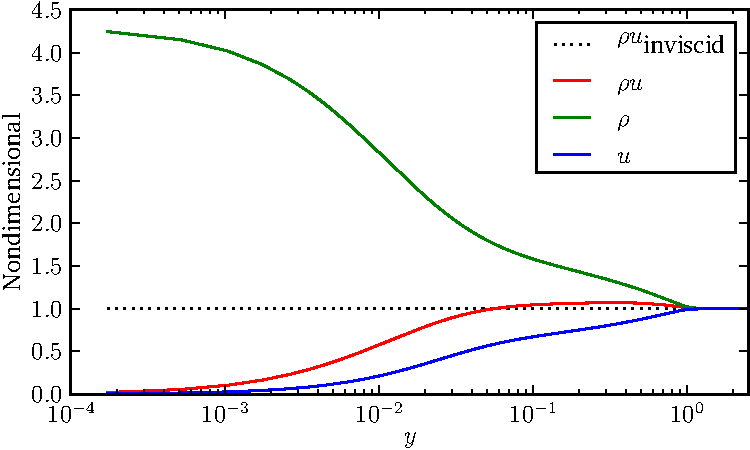
\includegraphics[width=\textwidth]{delta1weird}
        \\
        \small
        Case t4.134
    \end{column}
\end{columns}
\end{frame}

%===============================================================================
\subsection{Characterization of the Homogenized Boundary Layers}
%===============================================================================

\begin{frame}
    \frametitle{Inner scaling for simulations t3.199 and t4.134}
    \framesubtitle{Viscous sublayer and buffer layer but no
                   logarithmic region due to low $\Reynolds[\theta]{}$}
    \begin{center}
        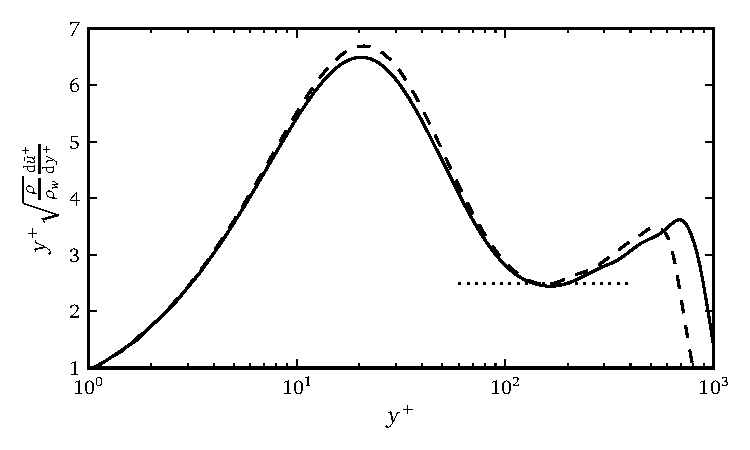
\includegraphics[width=0.7\textwidth]{hqd_inner}
        \\\vspace{-0.75em}
        \small
        Case t3.199 (dashed) and t4.134 (solid)
    \end{center}
    %
%   \vspace{1.5em}
%   Semi-local units by \citet{Huang1995Compressible}:
%   \begin{align}
%       \tau_w &= \left(\mu \partial_y u\right)_w
%       &
%       u_\tau^\ast &= \sqrt{\tau_w/\rho}
%       &
%       \delta_{\nu}^\ast   &= \nu/u_\tau^\ast
%   \end{align}
\end{frame}

\begin{frame}
    \frametitle{Stress contributions to the streamwise momentum}
    \framesubtitle{Reduced maximum relative to \citet{Topalian2014Temporal} due to favorable pressure gradient}
    \begin{center}
        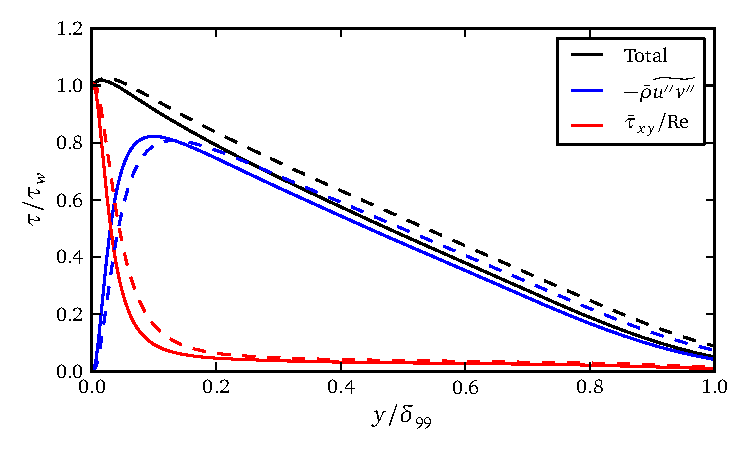
\includegraphics[width=0.7\textwidth]{hqd_tauxy}
        \\\vspace{-0.75em}
        \small
        Case t3.199 (dashed) and t4.134 (solid)
    \end{center}
\end{frame}

\begin{frame}
    \frametitle{Primitive and Reynolds stress profiles with uncertainty}
    \framesubtitle{%
        Maximum $\widetilde{{u^{\prime\prime}}^2}$
        higher than \citet{Guarini2000Direct,Coleman1995Numerical}\\
        consistent with wall blowing~\citep{Sumitani1995Direct}
        %Uncertainty per \citet{Oliver2014Estimating}.
    }
    \begin{columns}
        \begin{column}{0.5\linewidth}
          \centering
          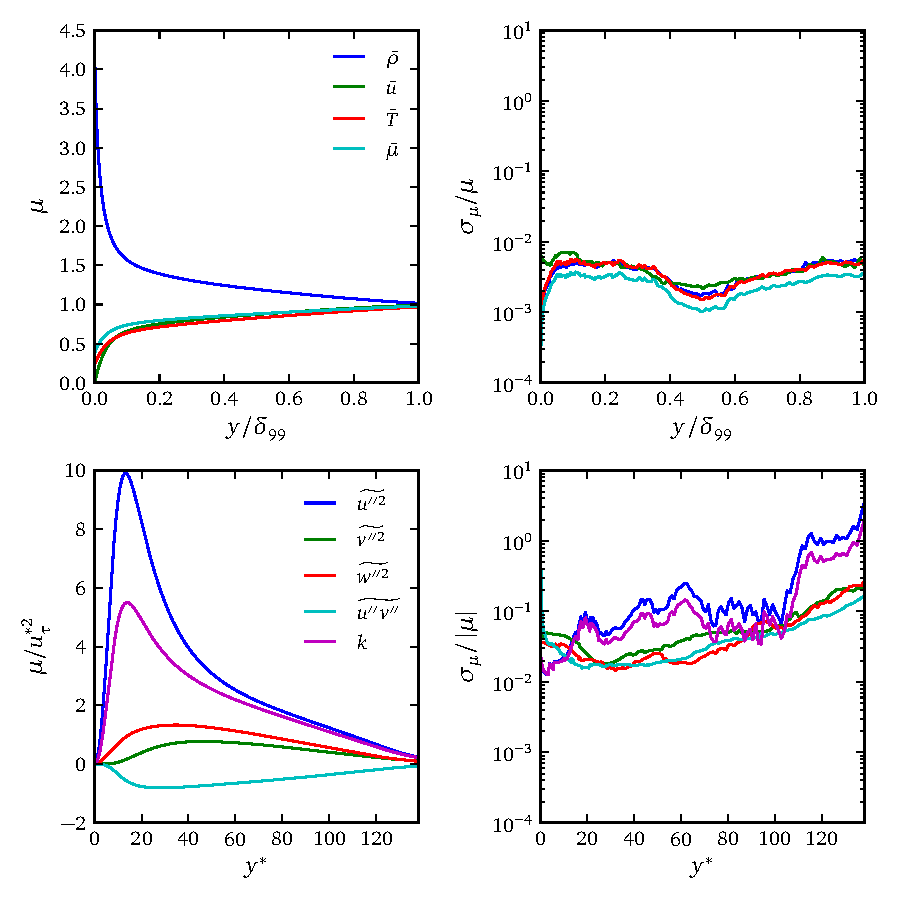
\includegraphics[width=\textwidth]{profile-t3199}
          \\
          Case t3.199
        \end{column}
        \begin{column}{0.5\linewidth}
          \centering
          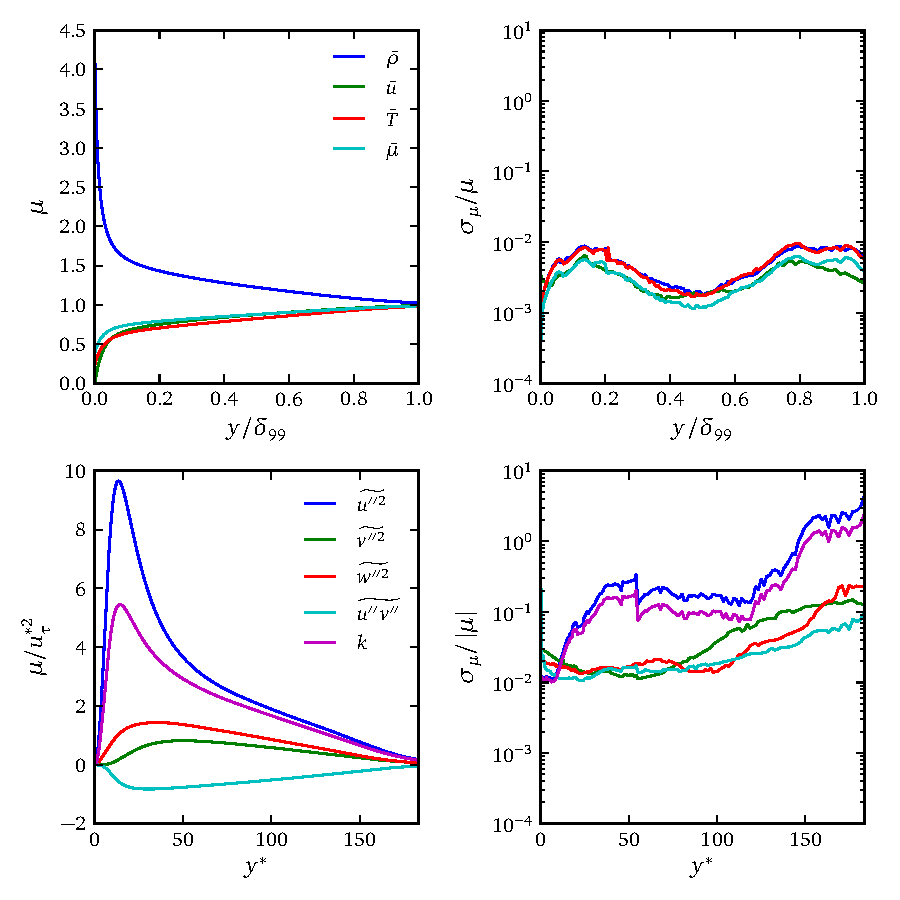
\includegraphics[width=\textwidth]{profile-t4134}
          \\
          Case t4.134
        \end{column}
    \end{columns}
\end{frame}

\begin{frame}
    \frametitle{Near-wall, root-mean-squared vorticity fluctuations}
    \framesubtitle{%
        Vs
        adiabatic-wall, $\Mach = 2.5$ by
        \citet{Guarini2000Direct} and incompressible by
        \citet{Spalart1988Direct}
    }
    \centering
    \vspace{0.1em}
    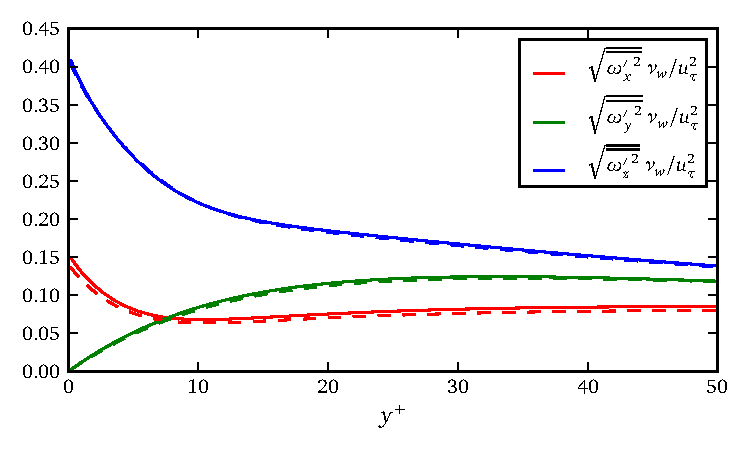
\includegraphics[width=0.55\textwidth]{hqd_vort}
    \\\vspace{-0.65em}
    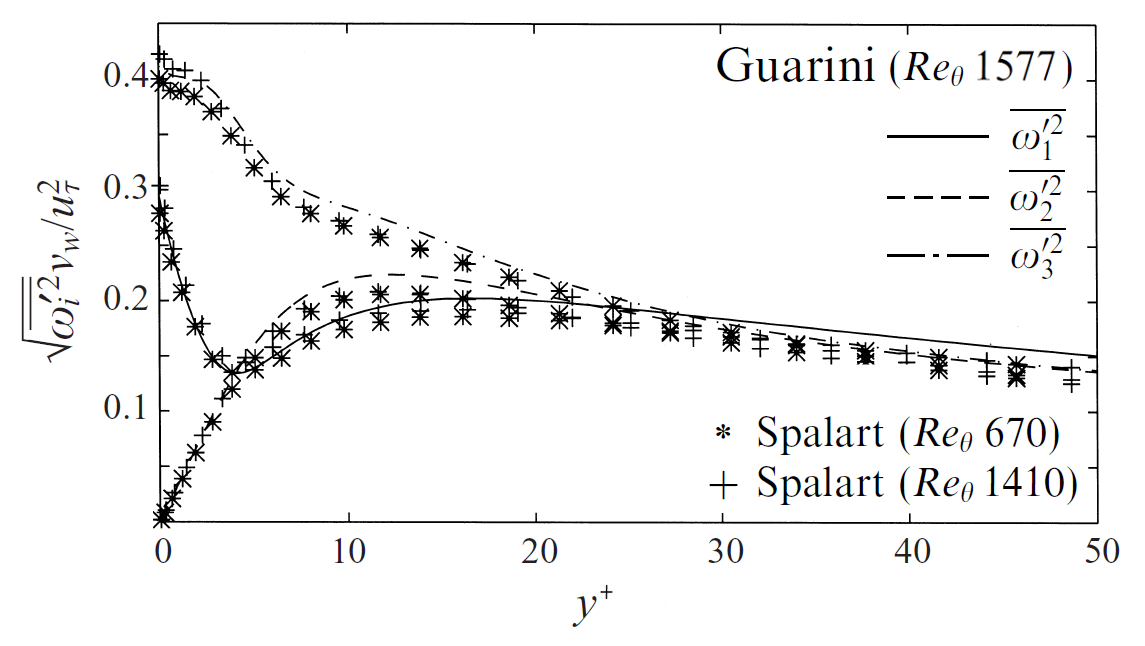
\includegraphics[width=0.57\textwidth]{GuariniJFM2000Figure8_Reworked}\hspace{1.15em}
\end{frame}

\begin{frame}
    \frametitle{Turbulent kinetic energy budgets}
    \framesubtitle{%
        Peak production lower than 0.25 found by \citet{Schlatter2009Turbulent} from ZPG at $\Reynolds[\theta]{}=670$
    }
    \begin{columns}
        \begin{column}{0.5\linewidth}
          \centering
          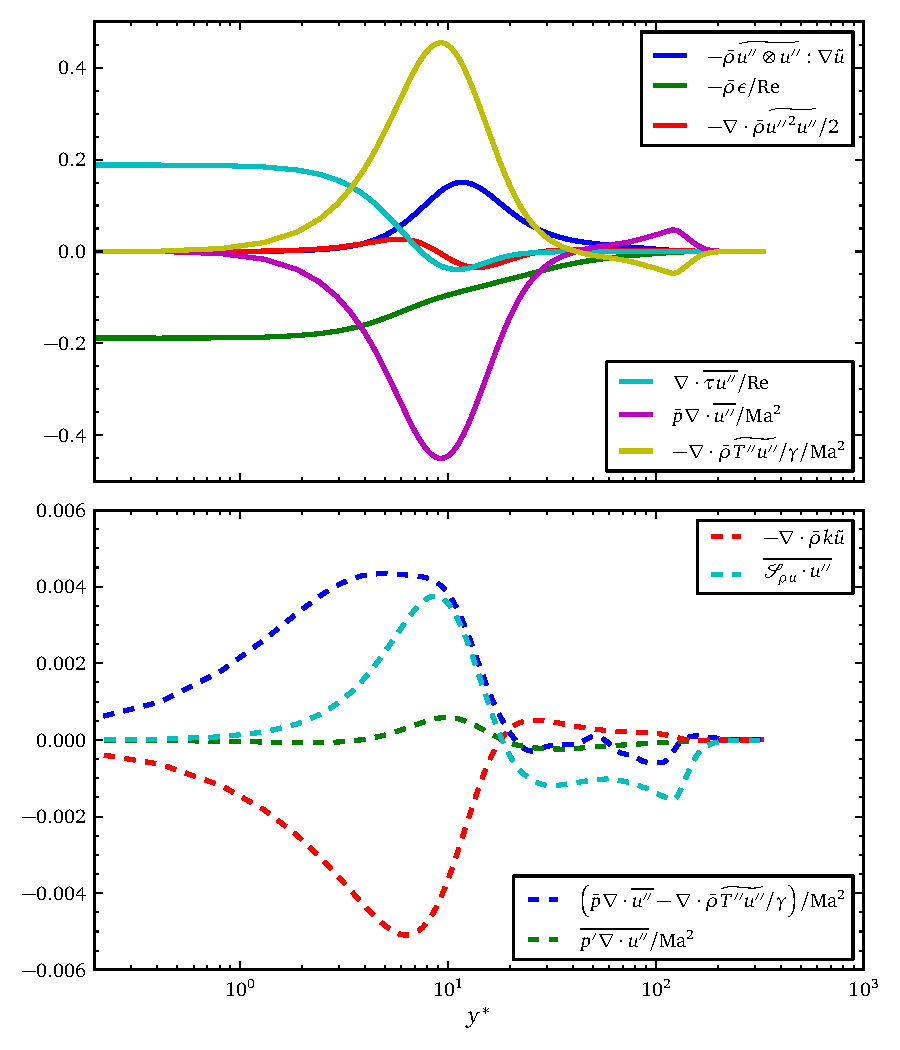
\includegraphics[width=\textwidth]{hqd_tke_t3199}
          \\\vspace{-0.5em}
          Case t3.199
        \end{column}
        \begin{column}{0.5\linewidth}
          \centering
          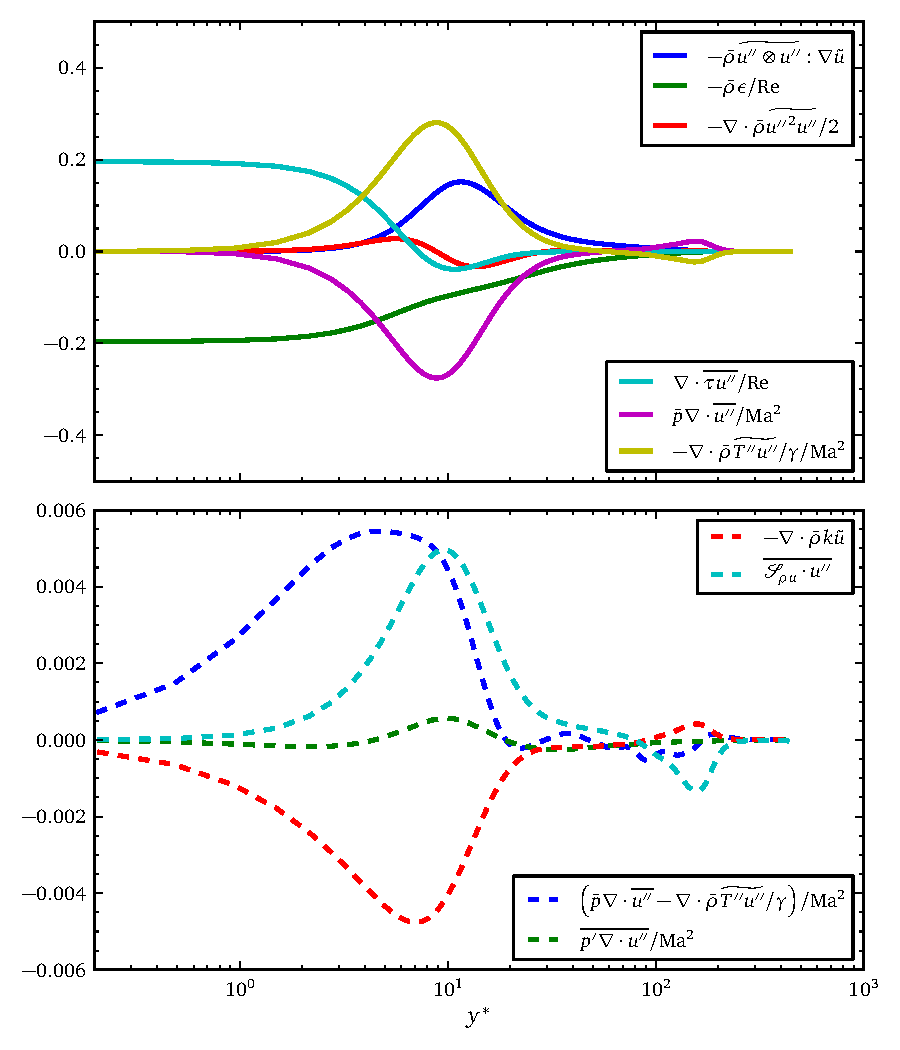
\includegraphics[width=\textwidth]{hqd_tke_t4134}
          \\\vspace{-0.5em}
          Case t4.134
        \end{column}
    \end{columns}
\end{frame}

\begin{frame}{Conclusions}
    \begin{enumerate}
        \item Created a new, well-verified, openly available Fourier/B-spline DNS framework
              already reused, in part or in full, by
              \citet{Malaya2012Estimating,
              Topalian2013Direct,
              Lee2013Petascale,
              Topalian2014Temporal,
              Topalian2014Spatiotemporal,
              Oliver2014Estimating,
              Lee2014Experiences,
              Lee2014Direct}
        \item Generated new, openly available DNS data with well-quantified certainties suitable for modeling and calibration purposes
        \item Simulations show significant cold wall, wall blowing, and favorable pressure gradient effects
        \item Near-wall vorticity fluctuations exhibit qualitatively different behavior than observed by \citet{Guarini2000Direct} or \citet{Spalart1988Direct}
        \item Small or negative displacement thicknesses present because of the cold wall
        \item Turbulent kinetic energy budget supports notion that spatiotemporally homogenized flows can serve as a convenient model problem for calibration
    \end{enumerate}
\end{frame}

%%%%===============================================================================
%%%\begin{frame}{\Large Proposed: Mapping regions that can sustain turbulence}
%%%\begin{columns}
%%%  \begin{column}{0.40\textwidth}
%%%    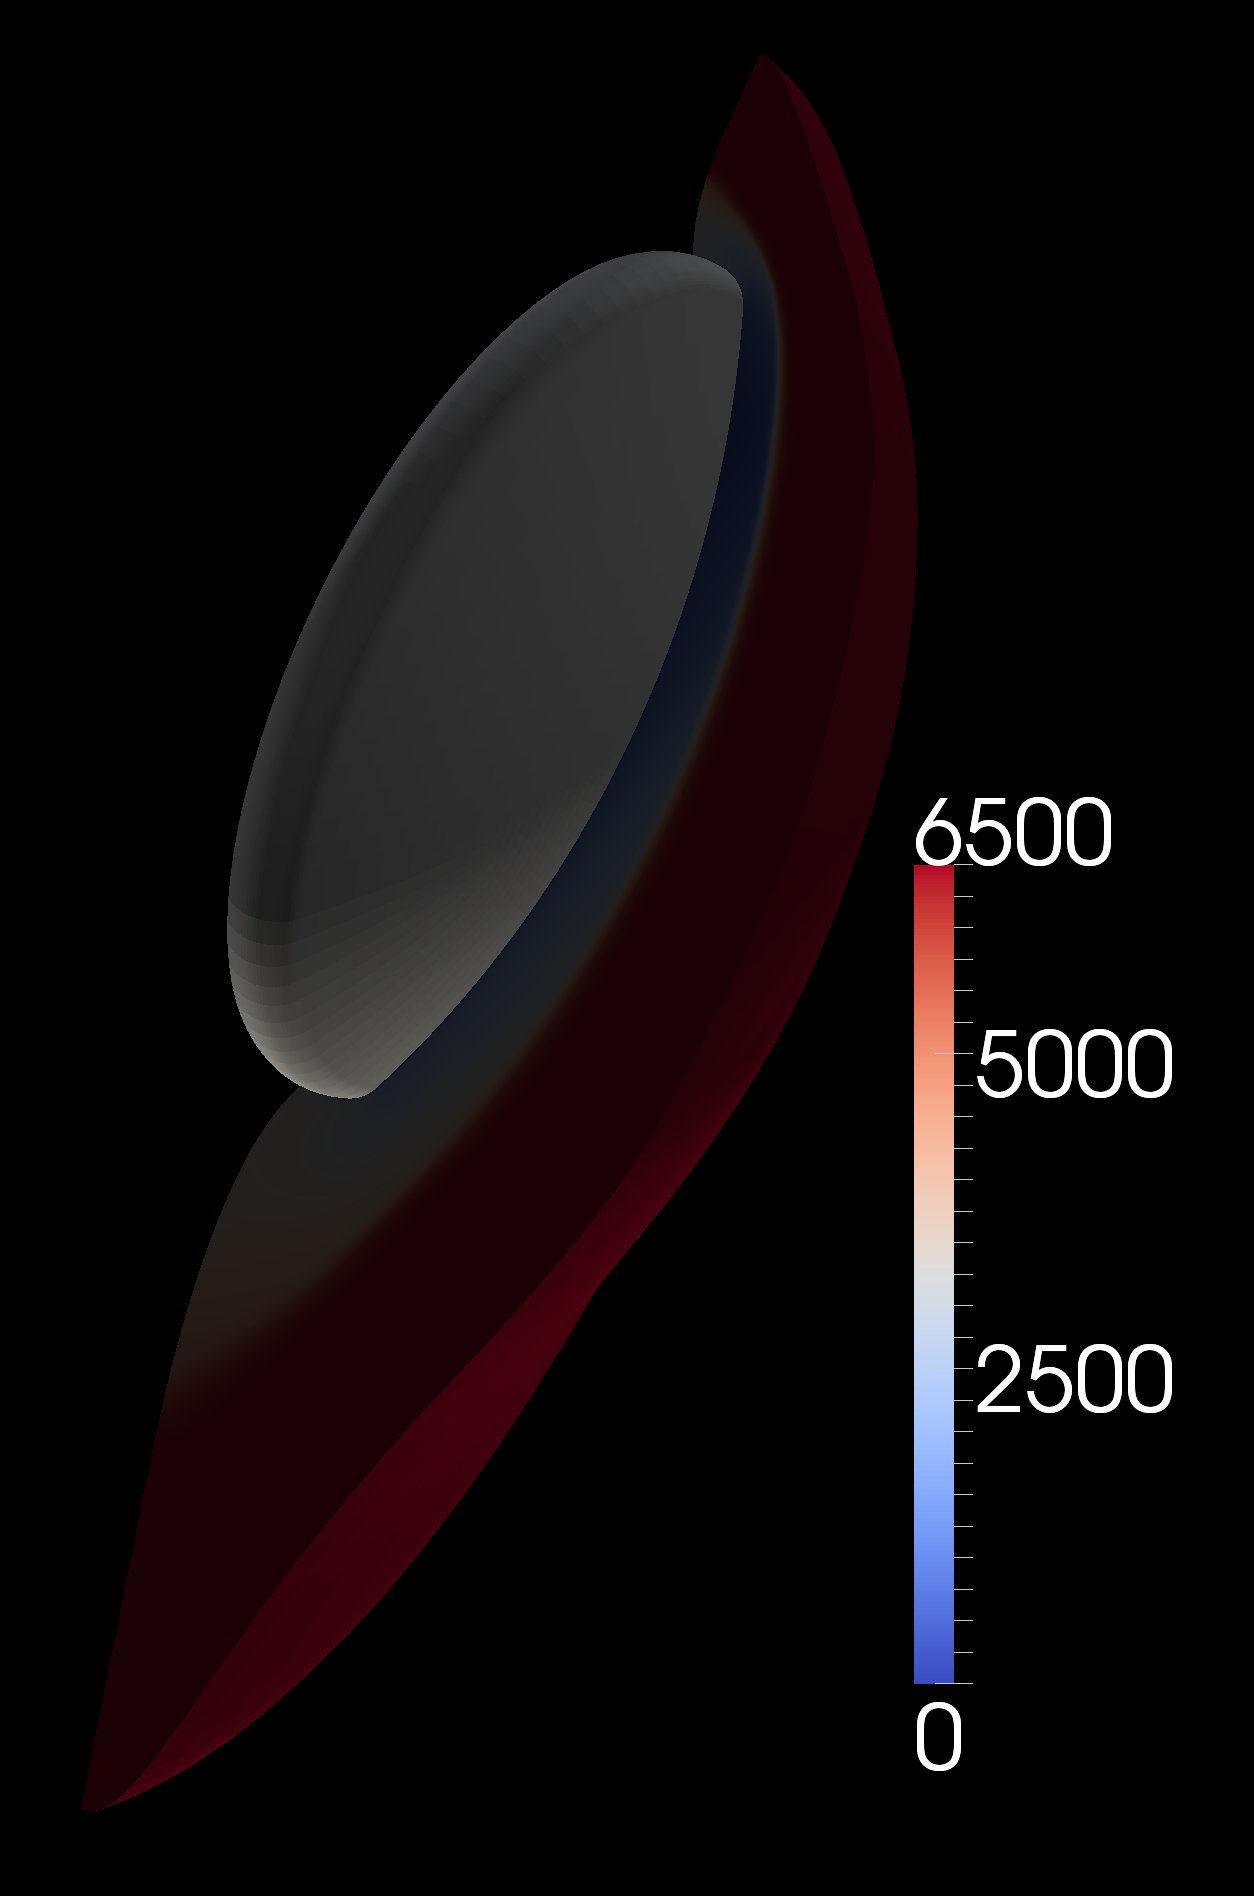
\includegraphics[width=0.90\textwidth]{cutaway_velocity_magnitude}
%%%    \\
%%%    \centering
%%%    courtesy Paul Bauman
%%%  \end{column}
%%%  \begin{column}{0.50\textwidth}
%%%    \small
%%%    At local conditions on the heat shield, when will turbulence
%%%    relaminarize?
%%%    \\\vspace{1em}
%%%    Local conditions being
%%%    \begin{itemize}
%%%       \item Reynolds number
%%%       \item Mach number
%%%       \item Pressure gradient strength
%%%       \item Wall transpiration rate
%%%       \item Edge-to-wall temperature ratio
%%%    \end{itemize}
%%%    traversed as a 1D parameter space
%%%    \\\vspace{1em}
%%%    Relaminarization defined in the spirit of
%%%    \citet{Narasimha1973Relaminarization,
%%%           Narasimha1979Relaminarization}
%%%    wrt impact on surface heat flux
%%%  \end{column}
%%%\end{columns}
%%%\end{frame}
%%%
%%%%===============================================================================
%%%\subsection{Work to be Completed}
%%%%===============================================================================
%%%
%%%%===============================================================================
%%%\begin{frame}{Sketch of remaining work}
%%%\small
%%%\begin{enumerate}
%%%  \item Analyze equation governing the evolution of nonlinear perturbation energy
%%%  \item Implement \emph{in situ} sampling of nonlinear perturbation energy budgets
%%%  \item Map heat shield scenario parameters of interest from laminar F.S.S.\\
%%%  \item Generate surface heat flux map for fully laminar conditions using Suzerain
%%%  \item Estimate grid and compute-time requirements for numerical study
%%%  \item If necessary, optimize code to permit study to proceed
%%%  \item Produce stationary simulation from conditions at edge of heat shield
%%%  \item Advance towards stagnation point using continuation-in-local-conditions,\\
%%%        assessing stationary/relaminarization using surface heat flux character
%%%  \item Repeat with additional grid to ensure results not numerical artifacts
%%%  \item Generate quantitative map of locations expected to be laminar during reentry
%%%  \item Analyze numerically obtained perturbation energy budgets
%%%  \item Reassess analysis to potentially produce relaminarization diagnostic
%%%  \item If successful, investigate predictive capabilities of proposed diagnostic
%%%\end{enumerate}
%%%\end{frame}

%%%%%%%%%%%%%%%%%%%%%%%%%%%%%%%%%%%%%%%%%%%%%%%%%%%%%%%%%%%%%%%%%%%%%%%%%%%%%%%%
\section{Reducing Transition-Driven Uncertainty}
%%%%%%%%%%%%%%%%%%%%%%%%%%%%%%%%%%%%%%%%%%%%%%%%%%%%%%%%%%%%%%%%%%%%%%%%%%%%%%%%

%%%%%%%%%%%%%%%%%%%%%%%%%%%%%%%%%%%%%%%%%%%%%%%%%%%%%%%%%%%%%%%%%%%%%%%%%%%%%%%%
\subsection{Motivation and Background}
%%%%%%%%%%%%%%%%%%%%%%%%%%%%%%%%%%%%%%%%%%%%%%%%%%%%%%%%%%%%%%%%%%%%%%%%%%%%%%%%

%%===============================================================================
%\begin{frame}{Ablation rate predictions are sensitive to transition\dots}
%\begin{center}
%  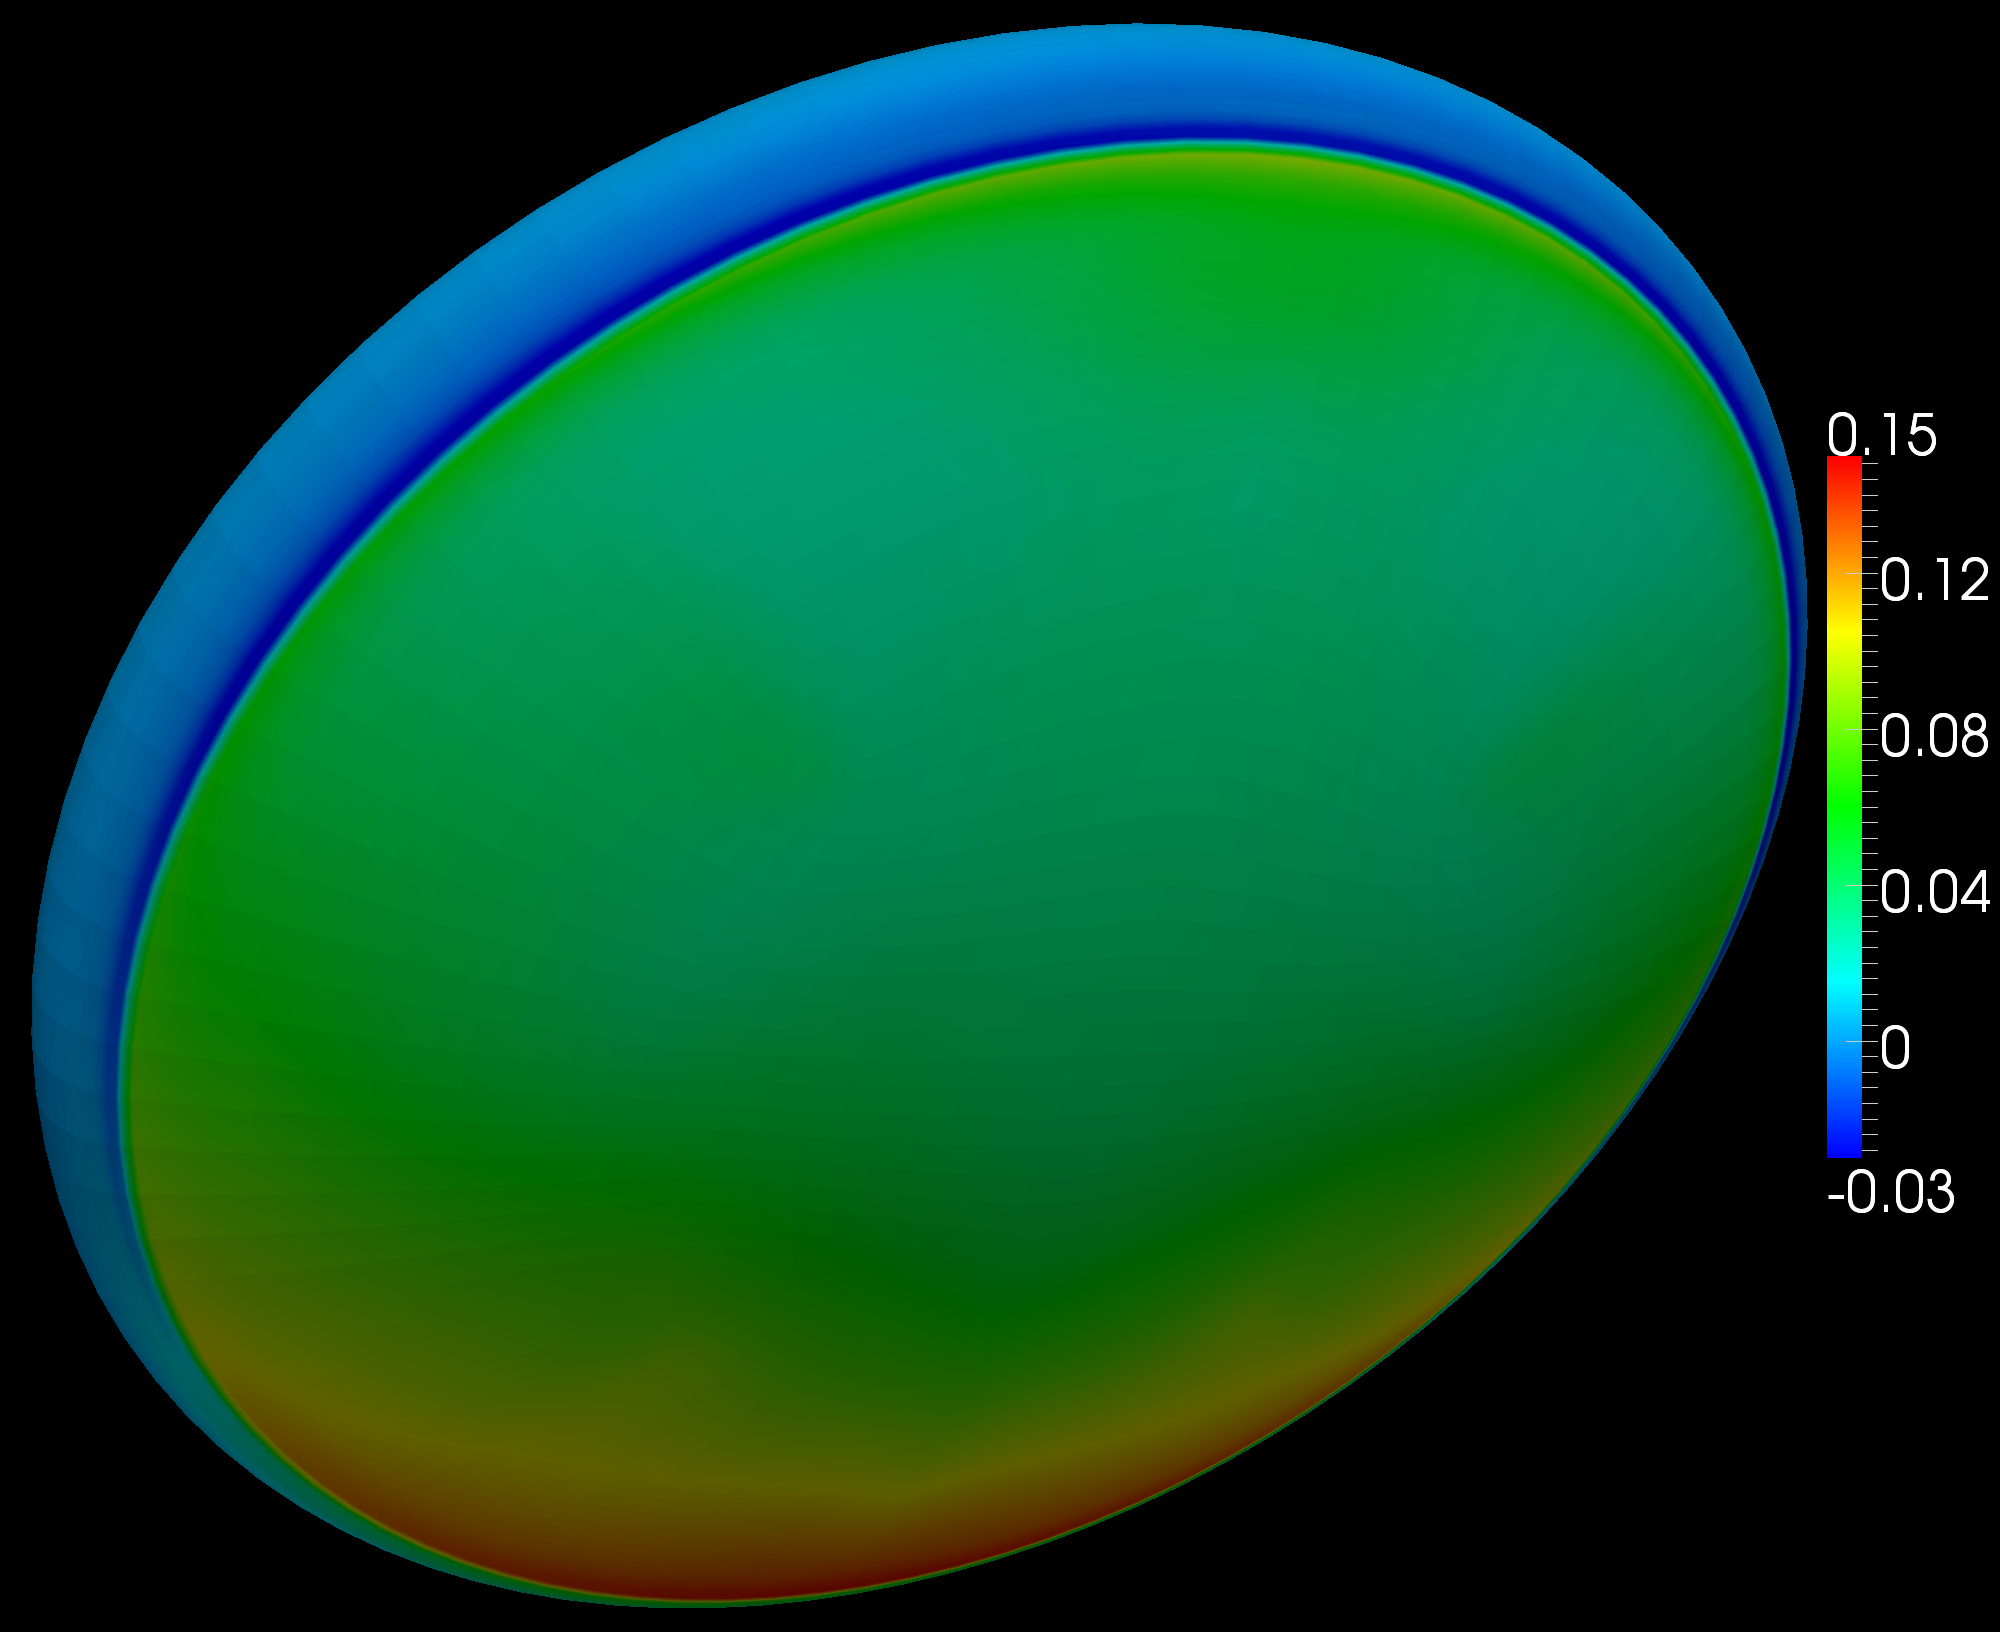
\includegraphics[width=0.65\linewidth]{normalized_difference}\\
%  Ablation $\displaystyle
%    \frac{   \dot{m}_\text{turbulent}
%           - \dot{m}_\text{laminar}  }
%         {   \max\left(\dot{m}_\text{turbulent}\right)}
%  $ during peak heating from ISS return
%  \begin{flushright}
%    courtesy Paul Bauman
%  \end{flushright}
%\end{center}
%\end{frame}

%===============================================================================
\begin{frame}{Ablation rate predictions are sensitive to transition\\
              and transition is sensitive to upstream environment}
\vspace{0.25em}
\begin{columns}[t]
  \begin{column}{.50\linewidth}
    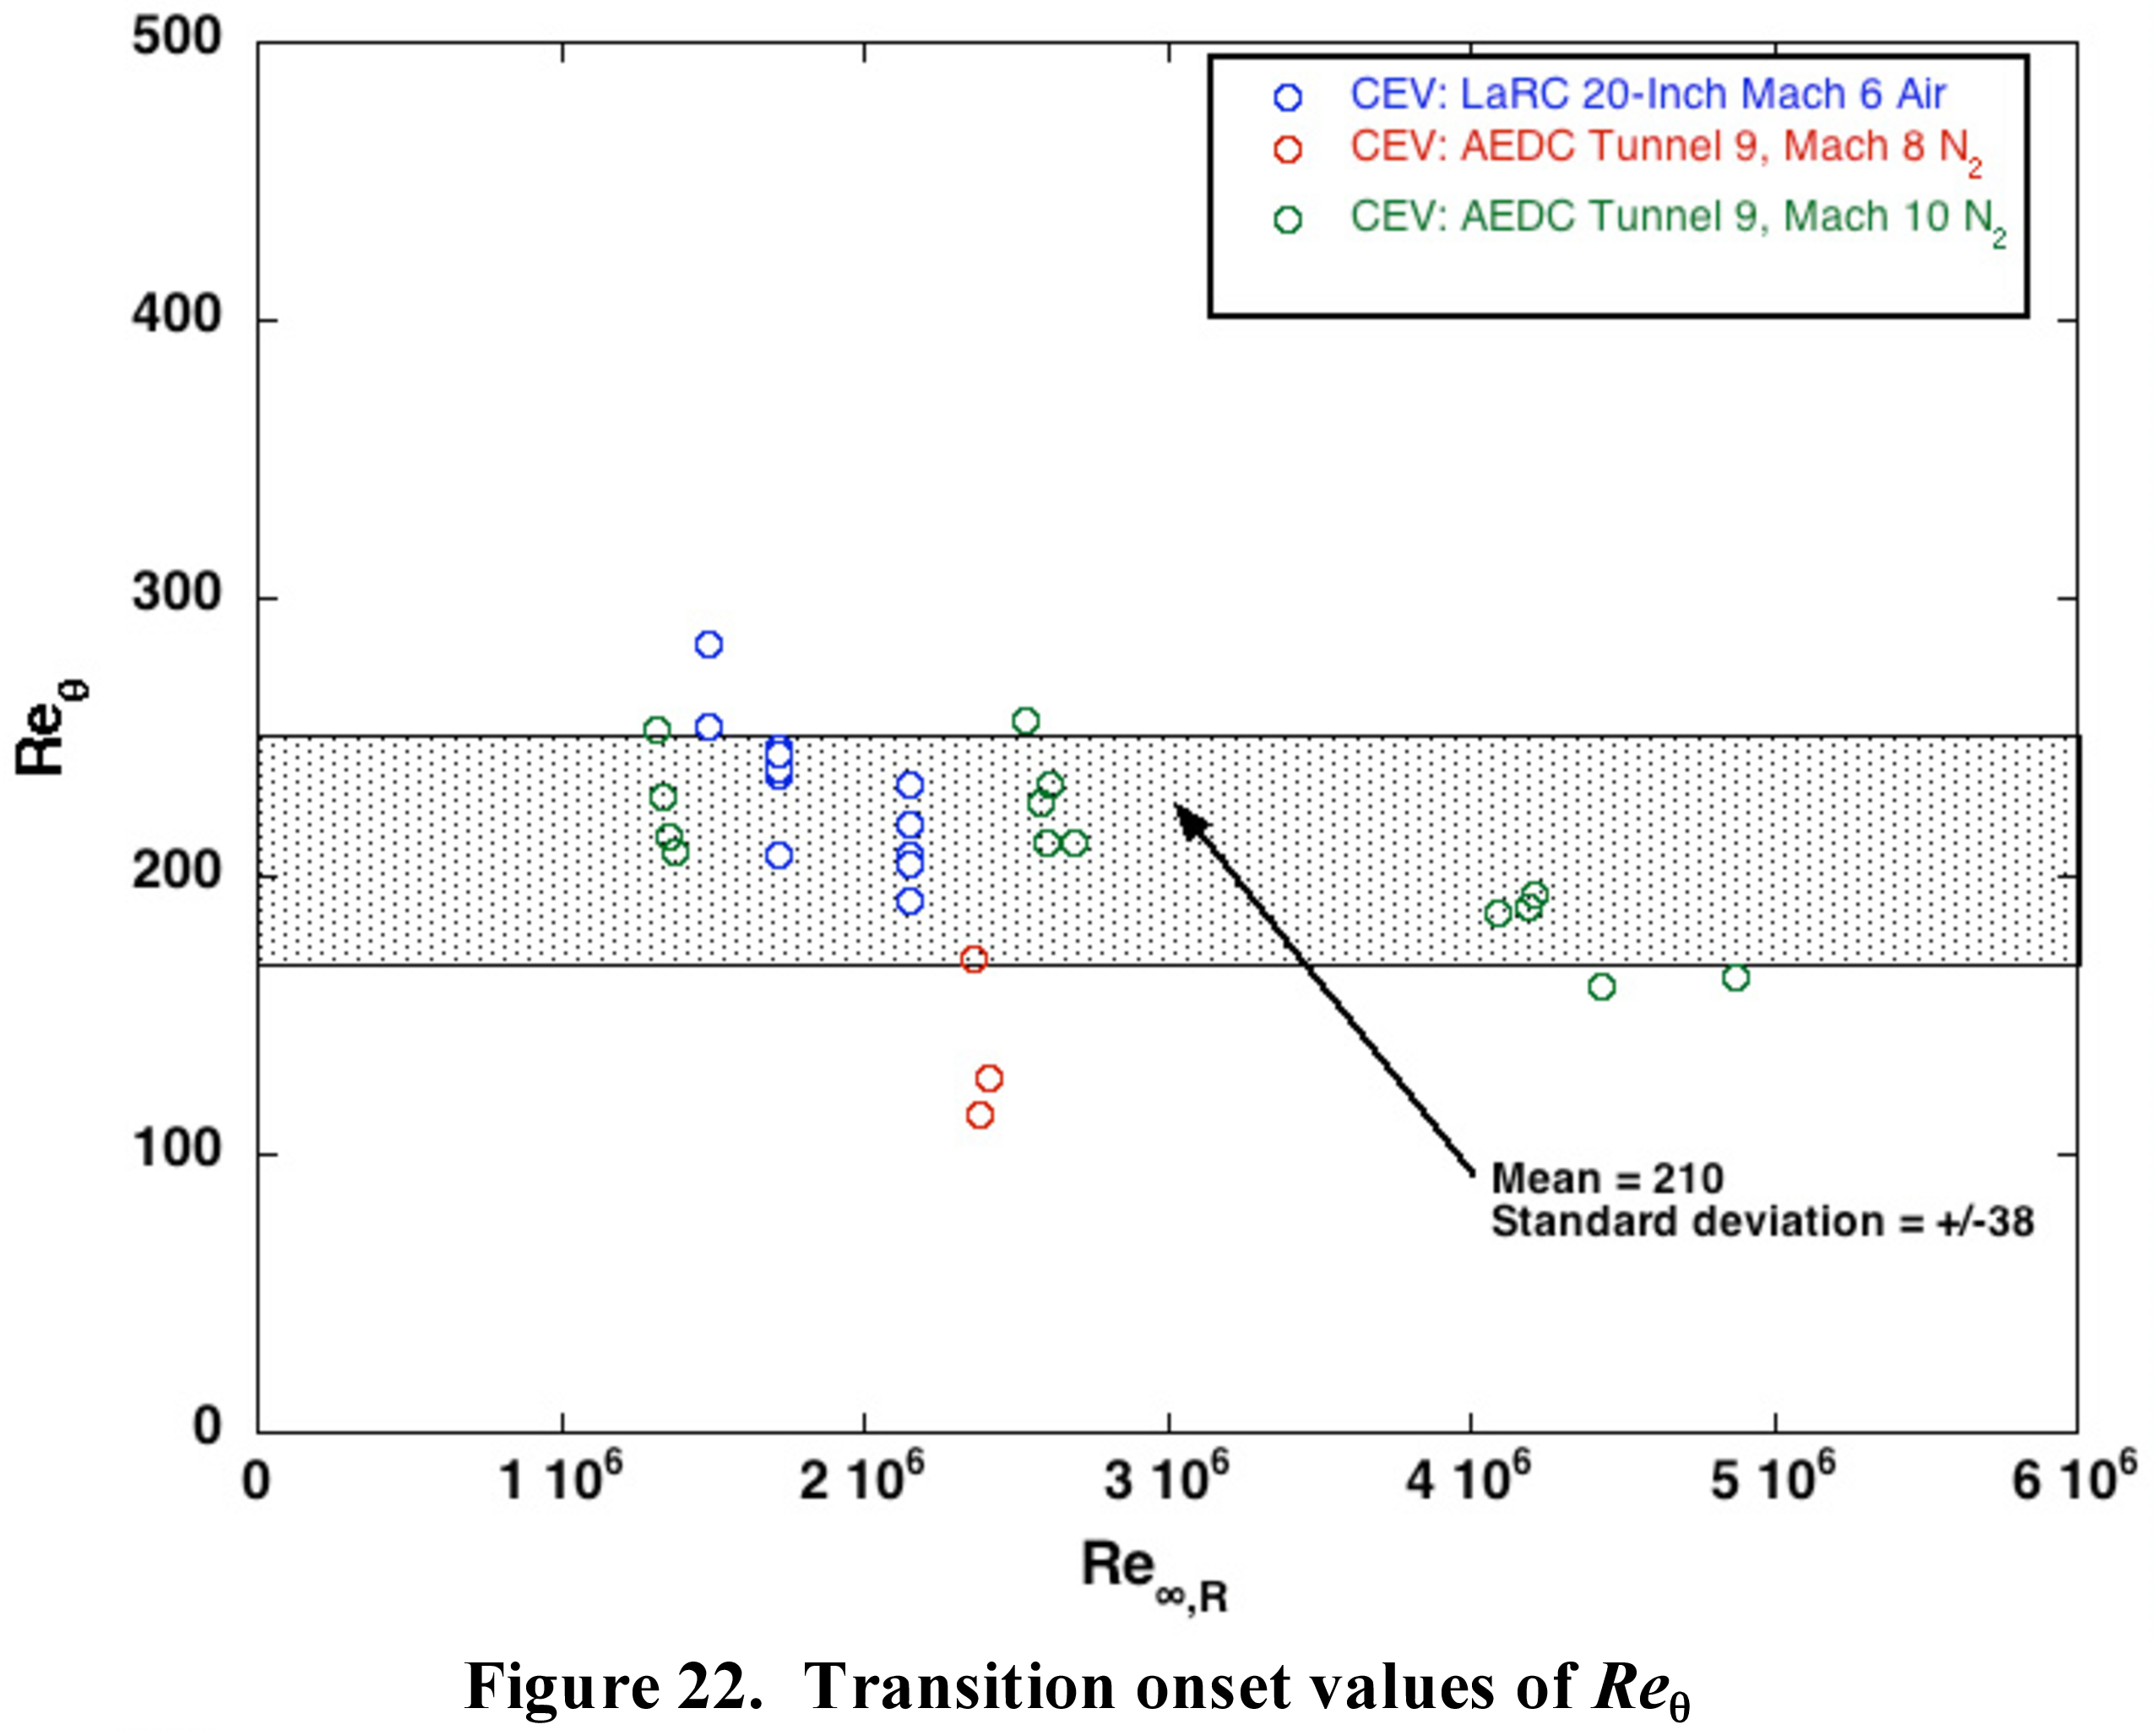
\includegraphics[width=0.99\linewidth]{Hollis2008_Figure22.png}\\
%%  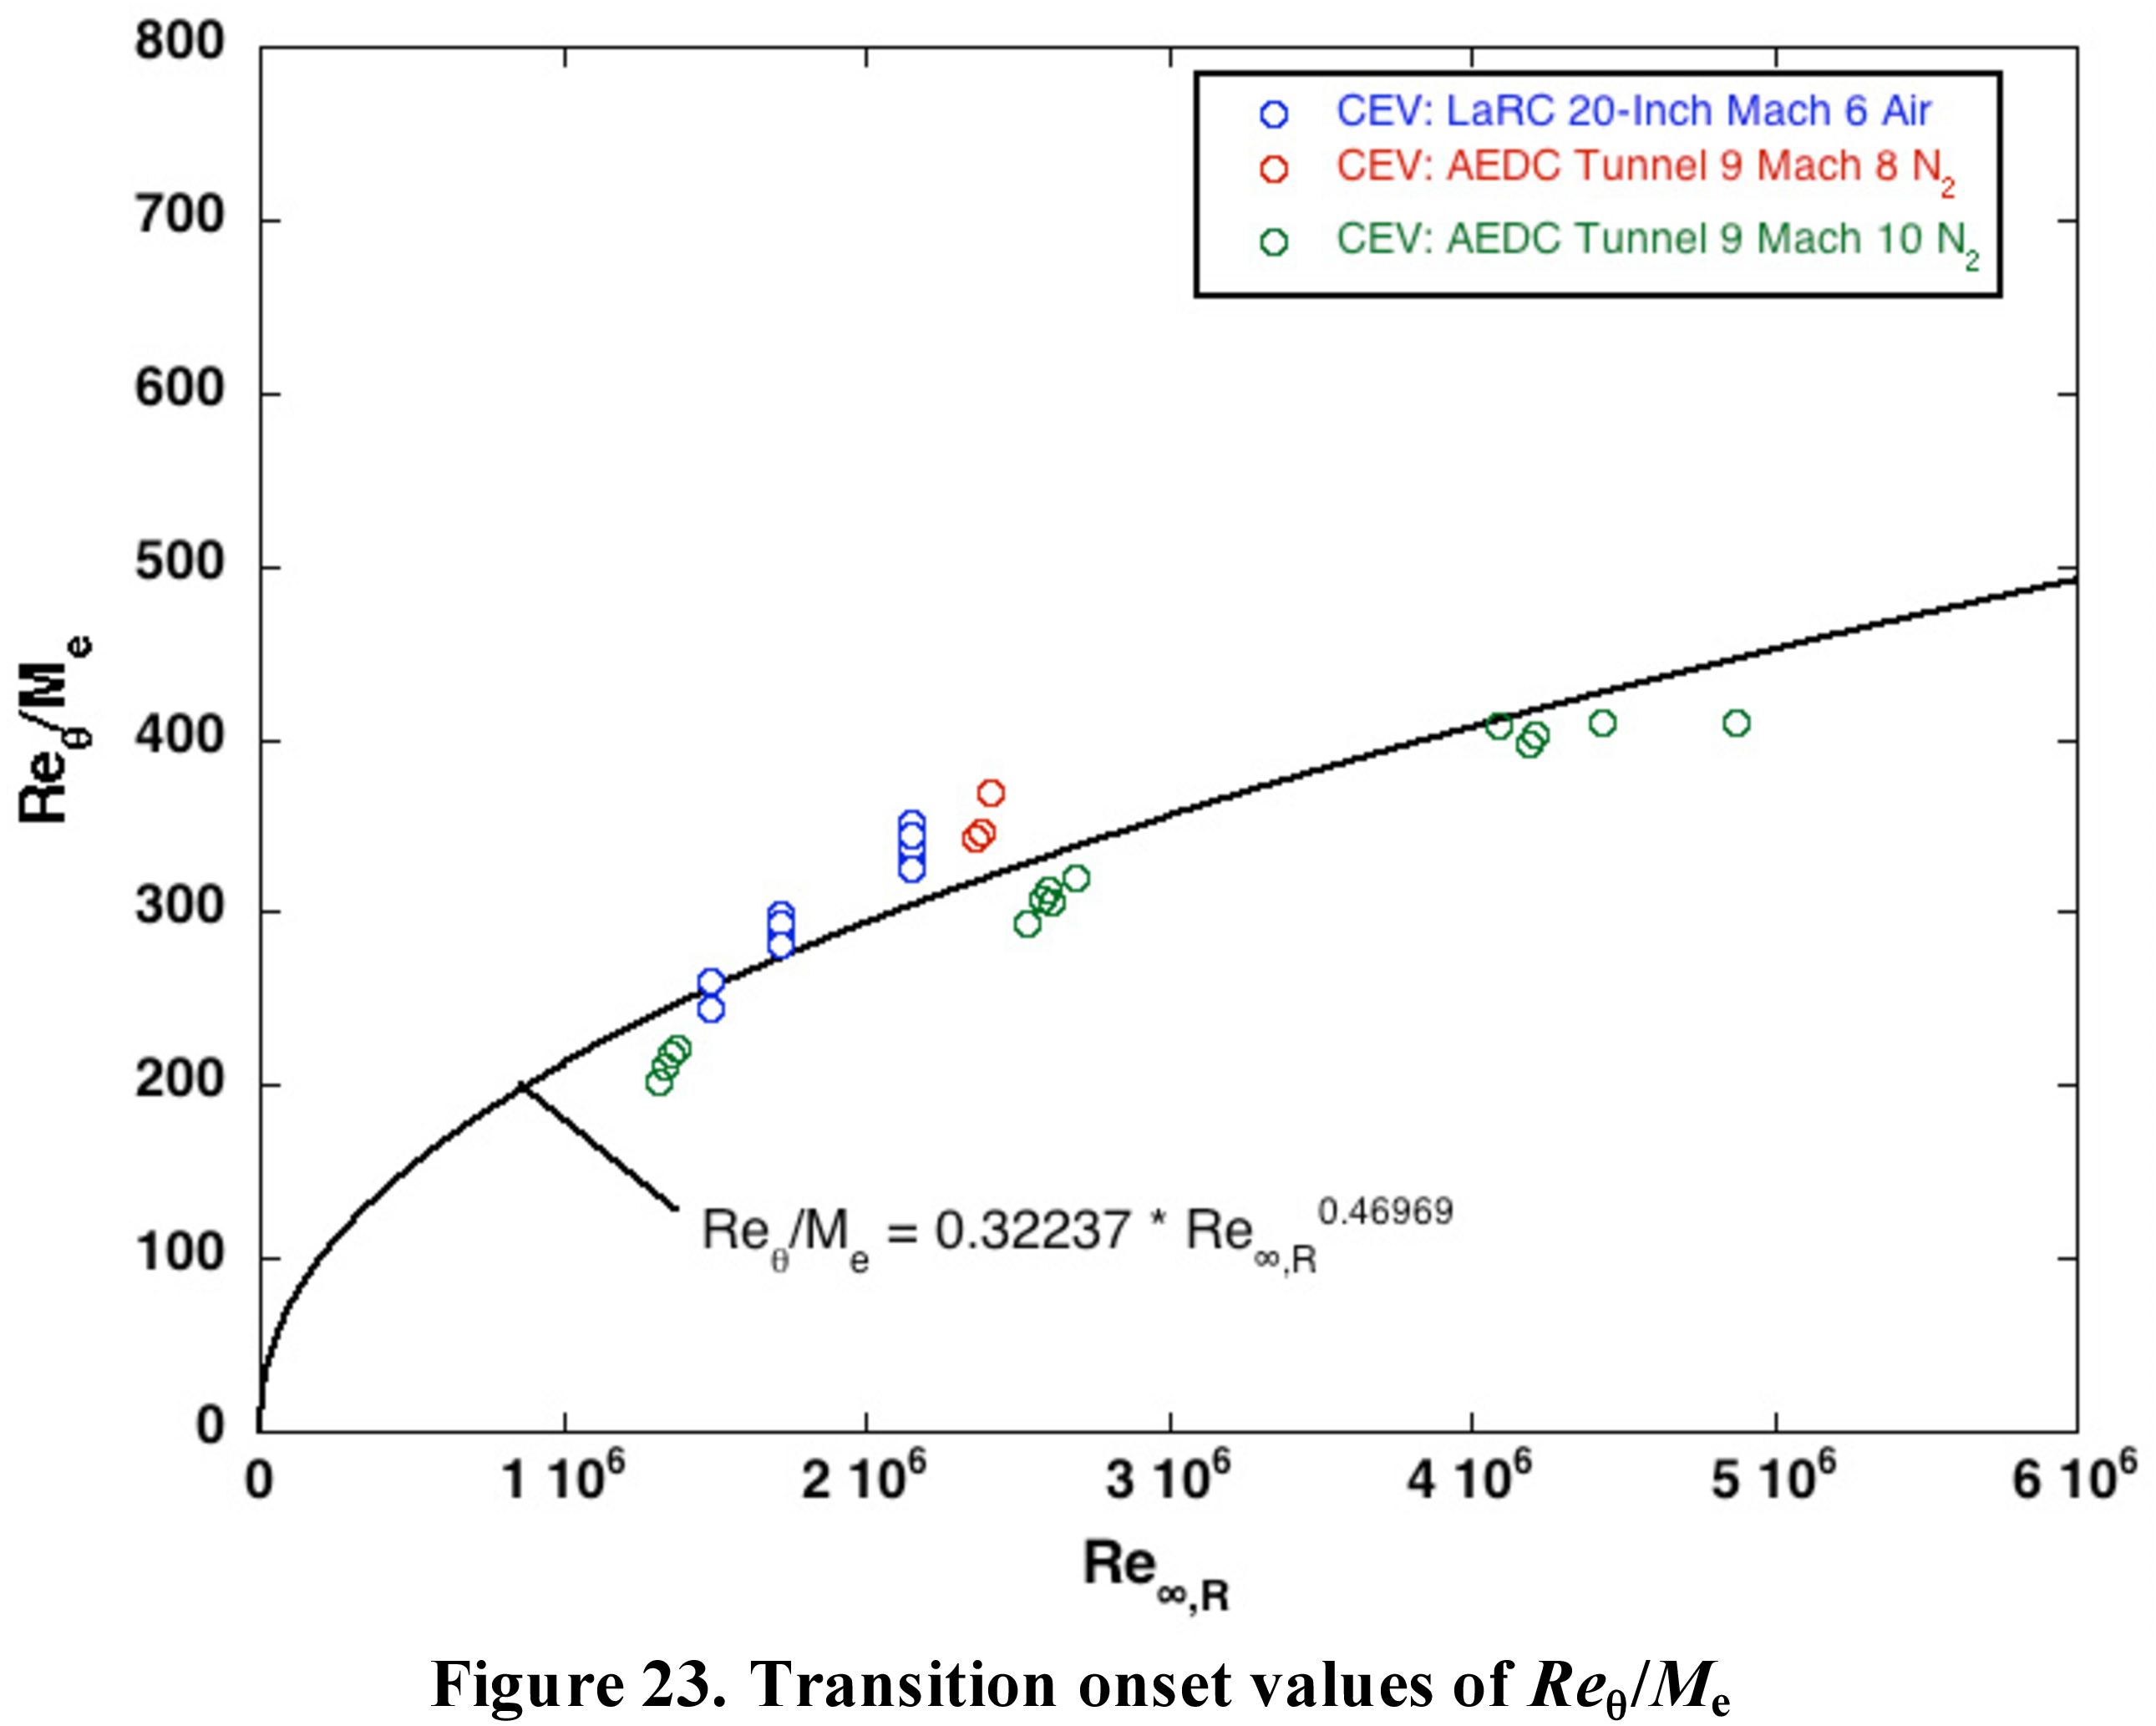
\includegraphics[width=0.99\linewidth]{Hollis2008_Figure23.png}\\
  \end{column}
\end{columns}
\small
\begin{quote}
  ``Because of the challenges associated with analysis of all the possible
  transition mechanisms, it is the defined policy of the [Orion MPCV]
  program to make a conservative assumption that the vehicle will
  experience turbulent flow throughout its trajectory.''
\end{quote}
\vspace{-2.5em}
\begin{flushright}
  from \citet{Hollis2008Aeroheating}
\end{flushright}
\end{frame}

%===============================================================================
\begin{frame}{}
\begin{columns}
  \begin{column}{0.30\textwidth}
    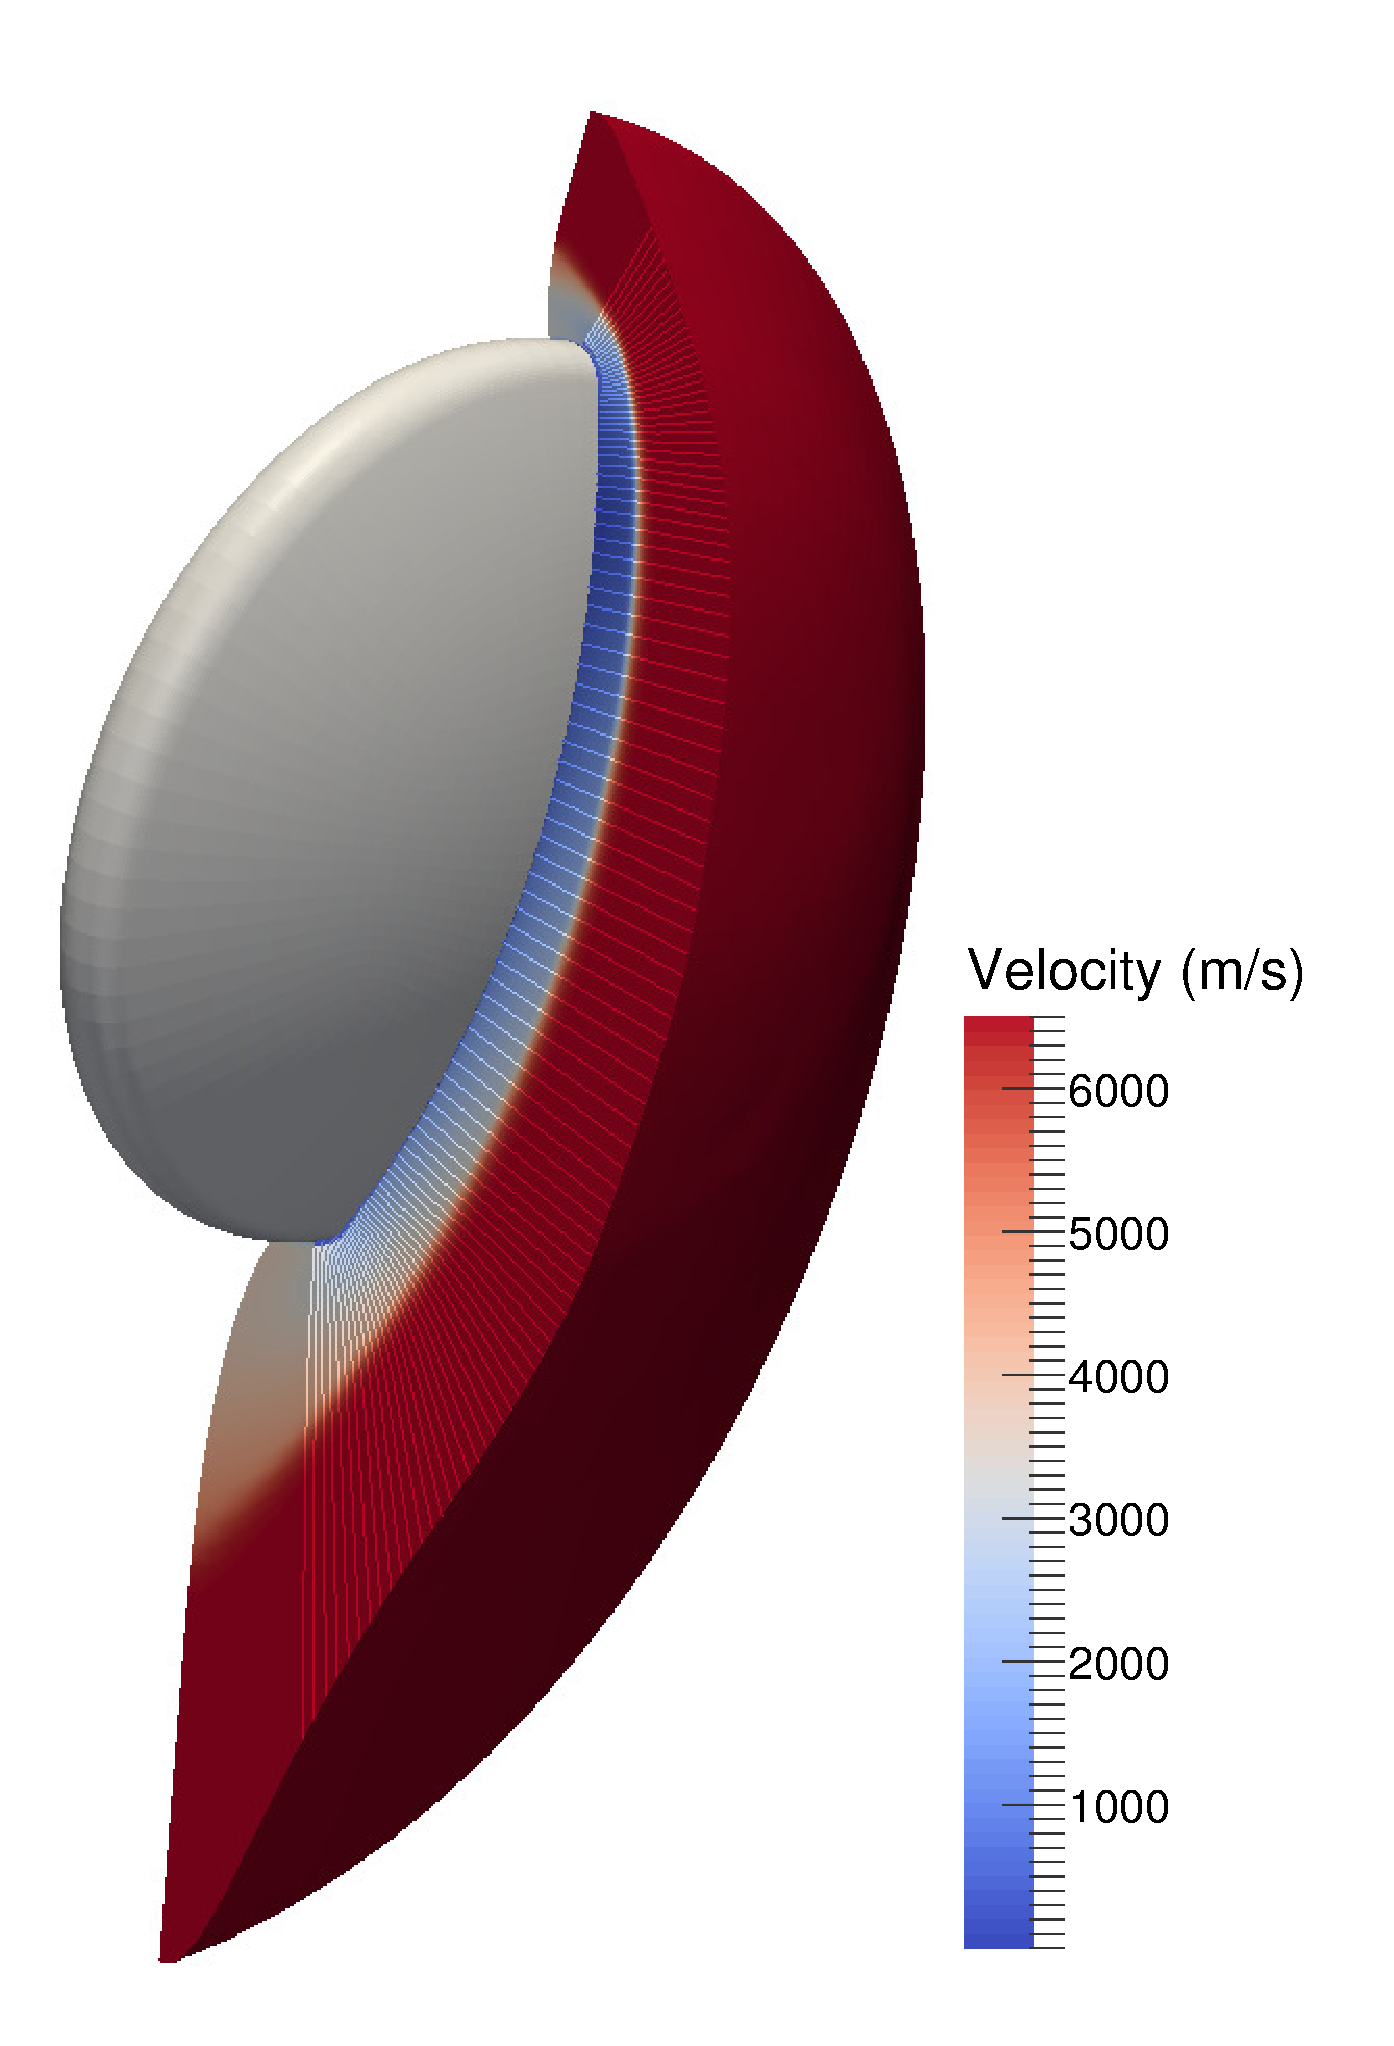
\includegraphics[width=\textwidth]{symplanenorm}
  \end{column}
  \begin{column}{0.75\textwidth}
  \begin{description}[Q]
    \item[Q] Where has transition occurred?
    \item[A] It depends\dots
      \begin{itemize}
        \item Freestream perturbation level
        \item Details of the bow shock
        \item Aerothermochemistry
        \item Outgassing of ablation products
        \item Ablator roughness due to fibrosity, spallation
      \end{itemize}
  \end{description}
  \vspace{1em}
  The heat shield is an incredibly noisy environment
  \\\vspace{1em}
  The unknowable details of that noise thwart answering
  this question well, let alone with much certainty
  \\\vspace{1em}
  For this reason, Orion MPCV project takes a conservative, assumed-turbulent
  approach
  \end{column}
\end{columns}
\end{frame}

%===============================================================================
\begin{frame}{}
\begin{columns}
  \begin{column}{0.30\textwidth}
    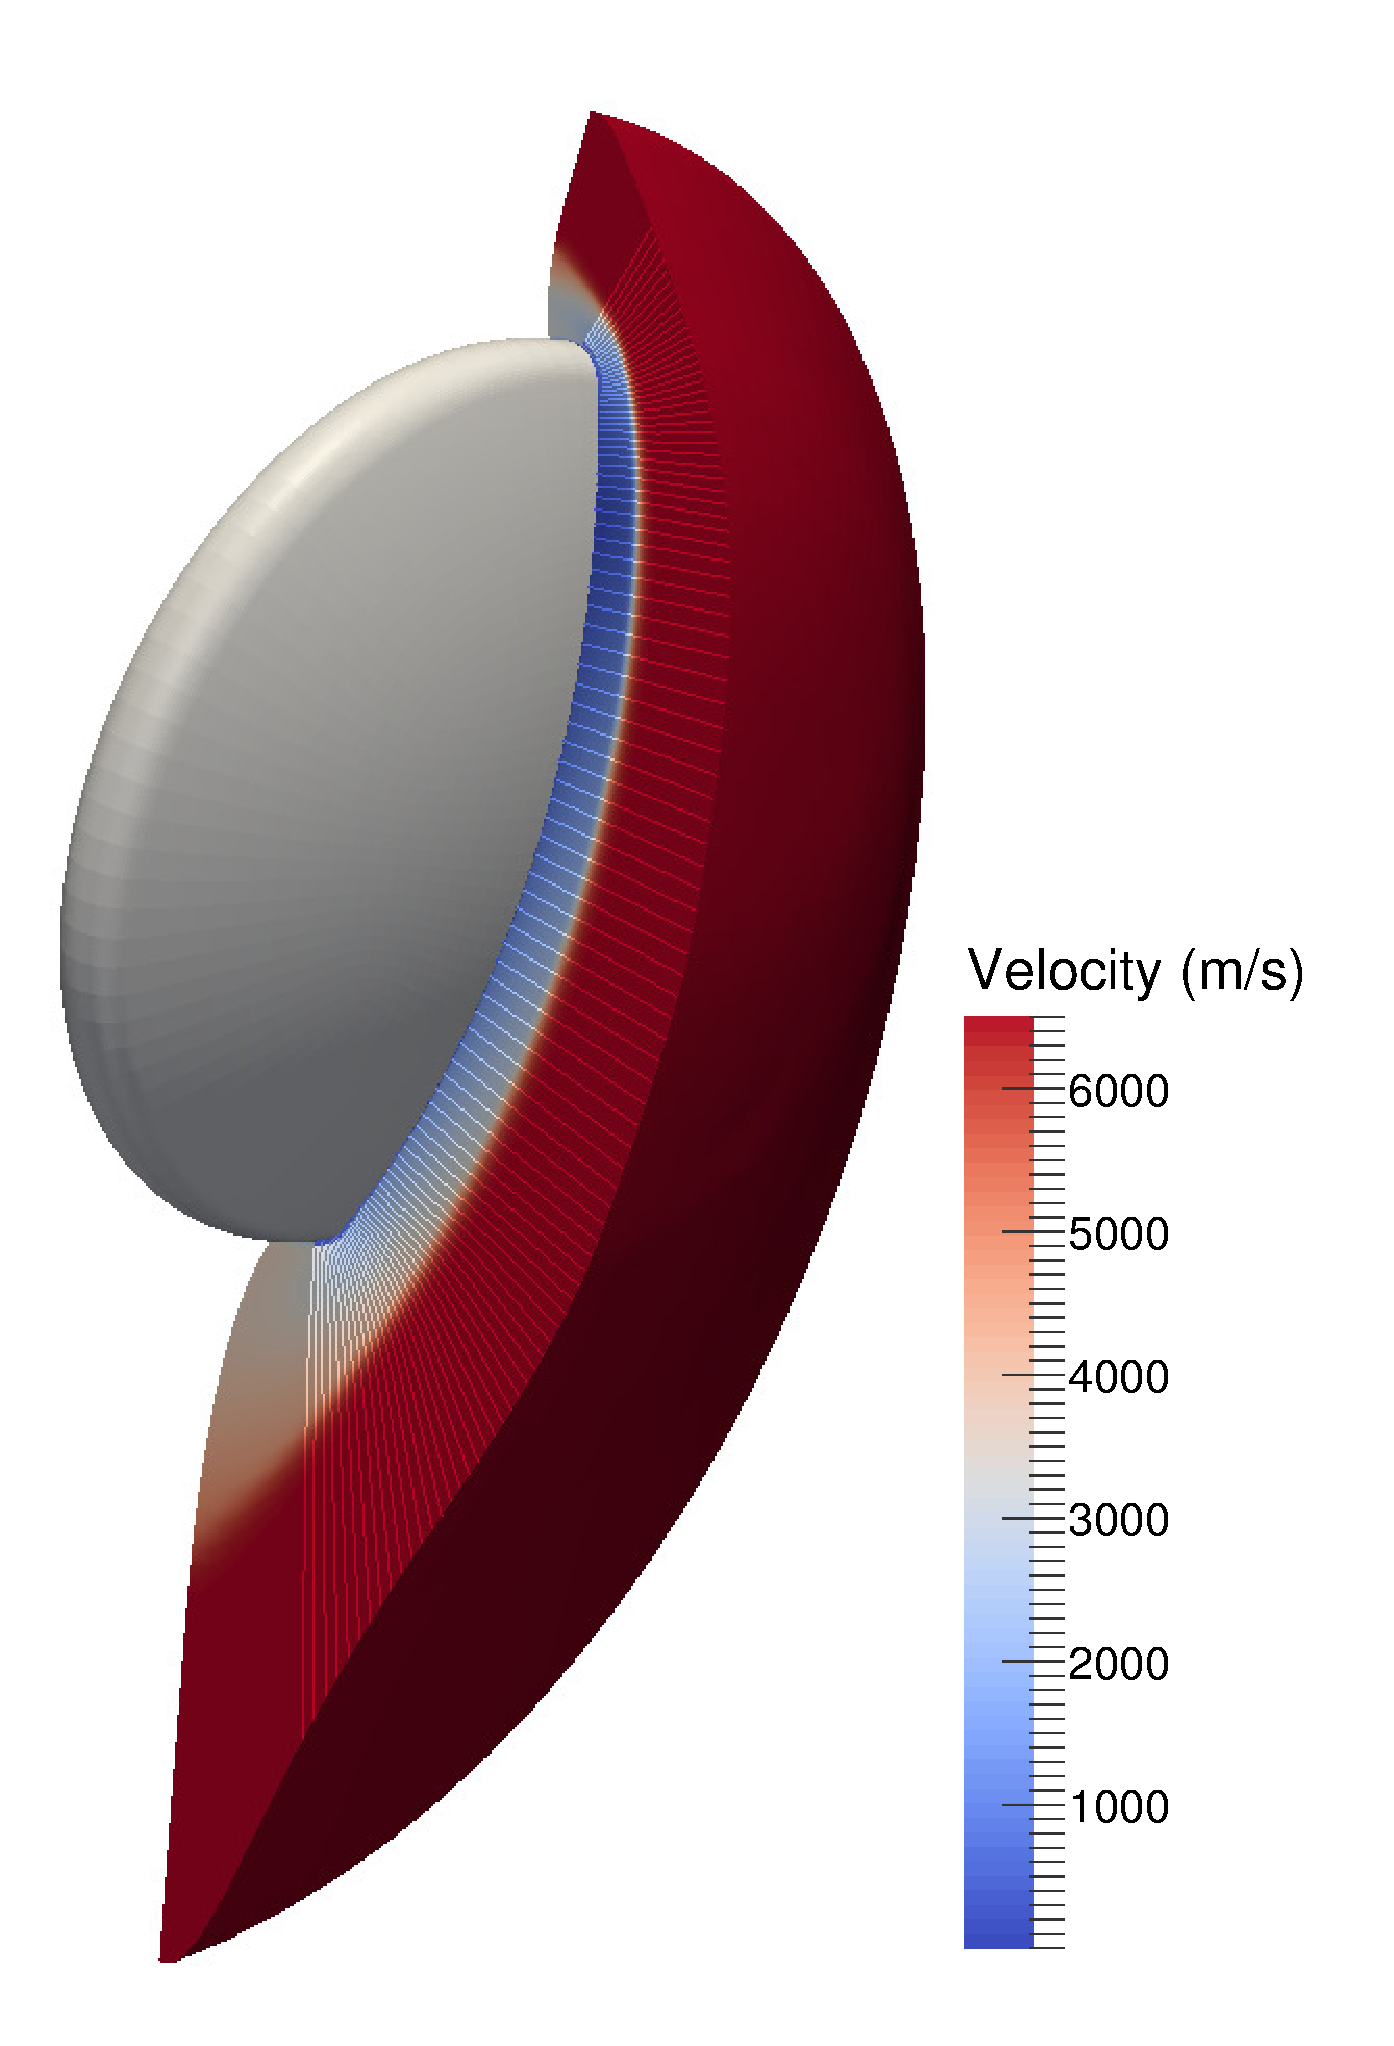
\includegraphics[width=\textwidth]{symplanenorm}
  \end{column}
  \begin{column}{0.75\textwidth}
  \begin{description}[<+->][Q]
    \item[Q] Where hasn't transition occurred?
    \item[A] The neighborhood of the stagnation point
    \item[A] Wherever local conditions can't sustain turbulence
        \medskip
        \begin{enumerate}[<+->]
            \item Turbulent boundary layer relaminarizes\\
                  \medskip
                  \begin{scriptsize}
                        \citet{Schraub1965Study},
                        \citet{Blackwelder1972Largescale},
                        \citet{Narasimha1973Relaminarization},
                        \citet{Narasimha1979Relaminarization},
                        \citet{Sreenivasan1982Laminarescent},
                        \citet{Iida1998Relaminarization},
                        \citet{Ichimiya1998Properties},
                        \citet{Talamelli2002Experimental},
                        \citet{Mukund2006Relaminarization},
                        \citet{Cal2008Similarity},
                        \citet{Bourassa2009Experimental}
                  \end{scriptsize}
                  \medskip
            \item Self-sustaining, nontrivial fluctuations can be found\\
                  \medskip
                  \begin{scriptsize}
                      Akin to being unstable per energy perturbation arguments
                  \end{scriptsize}
                  \medskip
        \end{enumerate}
  \end{description}
  \end{column}
\end{columns}
\end{frame}

\begin{frame}
\frametitle{Stability of fluids to arbitrary disturbances (\citet{Serrin1959Stability})}
\vfill
\small

\begin{block}{Incompressible Navier--Stokes equations with prescribed boundary}
\vspace{-1em}
\begin{align}
    \partial_t v + \nabla\cdot{}v\otimes{}v
&=
  - \rho^{-1} \nabla{} p
  + \nu \Delta{}v
  + f
&
  p, v &\in \Omega
  ,
\\
  v &= v_0
&
  v &\in \partial\Omega
\end{align}
\end{block}

\begin{block}{For any admissible $v'$, the perturbation $u = v' - v$ satisfies}
\vspace{-1em}
\begin{align}
  \partial_t u
&=
  \partial_t v'
  -
  \partial_t v
&
  u &\in \Omega
  ,
\\
  u &= 0
&
  u &\in \partial\Omega
\end{align}
\end{block}

\begin{block}{Smoothness and R.T.T. $\implies$ perturbation energy $E=u^2/2$ obeys}
\vspace{-1em}
\begin{align}
  \frac{\mathrm{d}}{\mathrm{d}t} \int_\Omega E
&=
  \int_\Omega \left(
      u \cdot \left[\frac{1}{2}\left(\nabla v + \trans{\nabla v}\right)\right] \cdot u
      - \Reynolds^{-1} \nabla u : \nabla u
  \right)
\end{align}
\end{block}

{%
    \footnotesize{}
    Theory extended by
    \citet{Joseph1965Stability, Joseph1966Nonlinear},
    \citet{Dudis1971Ekman, Dudis1971Buoyancy},
    \citet{Davis1973Reformulation},
    \citet{Galdi1983Local},
    \citet{Maremonti1984Asymptotic},
    \citet{Galdi1985Nonlinear},
    \citet{Galdi1990New},
    \citet{Padula1997Existence},
    \citet{Padula2000Stability},
    \citet{Padula2011Asymptotic}
}

\end{frame}


%===============================================================================
\begin{frame}{Research Objective}
    \begin{columns}[c,onlytextwidth]
    \begin{column}{.35\linewidth}
        Reduce transition-driven uncertainty by detecting
        the regions on an ablative heat shield that can sustain turbulence
    \end{column}
    \begin{column}{.65\linewidth}
        \vspace{-3em}
        \begin{flushright}
            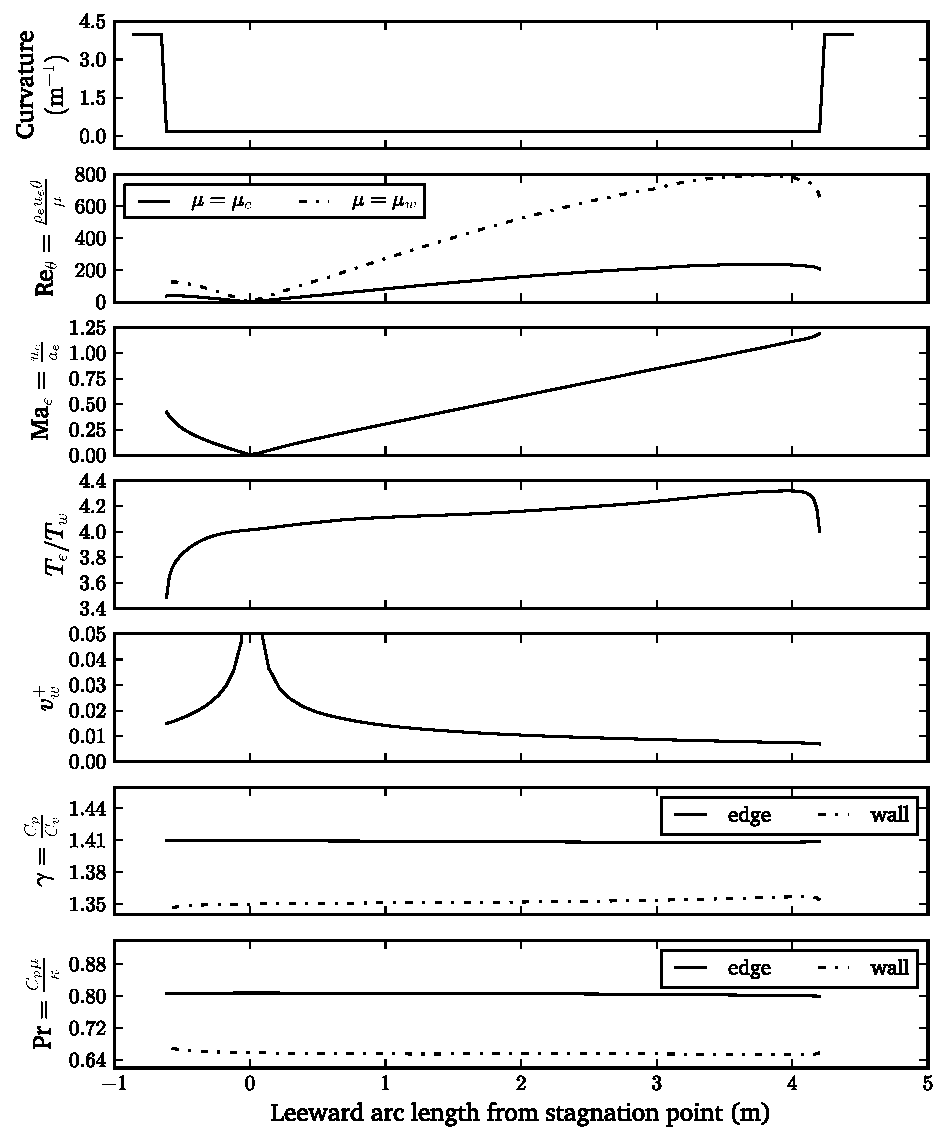
\includegraphics[height=0.99\textheight]{cevisslam_summary1}
        \end{flushright}
    \end{column}
    \end{columns}
\end{frame}

%%%%%%%%%%%%%%%%%%%%%%%%%%%%%%%%%%%%%%%%%%%%%%%%%%%%%%%%%%%%%%%%%%%%%%%%%%%%%%%%
\subsection{Results: Refining from Coarse Exploratory Simulations}
%%%%%%%%%%%%%%%%%%%%%%%%%%%%%%%%%%%%%%%%%%%%%%%%%%%%%%%%%%%%%%%%%%%%%%%%%%%%%%%%

\begin{frame}{Local conditions from the fully laminar Orion MPCV}
%
\begin{center}
\begin{tabular}{cccccc}
Location                              &
$\textrm{Re}_{\theta}$                & % Re_theta
$\textrm{Ma}_{e}$                     & % Ma_edge
$T_{e}/T_w$                           & % T_ratio
$v_w^{+}$                             & % v_wallplus
\raisebox{0.10ex}{$p_{e,\xi}^{\ast}$}   % p_exi
\\
\toprule\toprule
%Location  &  Re_theta  &  Ma_edge  &  T_ratio &  v_wallplus  &  p_exi          \\
4.134~m    &  223       &  1.15\z   &  4.29    &  0.00718     &  \num{-0.0123}  \\
3.199~m    &  225       &  0.899    &  4.26    &  0.00839     &  \num{-0.0102}  \\
2.299~m    &  177       &  0.660    &  4.18    &  0.00977     &  \num{-0.0127}  \\
1.389~m    &  114       &  0.411    &  4.13    &  0.0123\z    &  \num{-0.0179}
\end{tabular}
\end{center}
%
\vfill
%
Coarse simulations ($\Delta{}x^{+} \approx 30$) sustained fluctuations at each location:
\begin{itemize}
    \item Coarse grids suppress proper dissipation of turbulent kinetic energy
    \item Stationary turbulent production, Reynolds stresses, skin friction, etc.
    \item Stationary boundary layer thickness such that
          domain was $10\delta \times 2.5\delta \times 3\delta$
    \item Long correlations relative to $\delta$ unlike real turbulent boundary layers
    \item These fields are ``admissible $v'$'' per the energy perturbation method
\end{itemize}
%
\end{frame}

%===============================================================================
\begin{frame}
    \frametitle{Location 4.134~m}
    \framesubtitle{$\Delta{}x^{+}\approx{}18.7$ and $\Delta{}z^{+}\approx{}11.2$}
    %
    \begin{columns}[c,onlytextwidth]
    \begin{column}{.35\linewidth}
        \scriptsize
        %
        Refinement to production\\resolution at $t=0$
        \\\bigskip
        %
        Mean freestream flow\\traverses $L_x$ roughly\\every $\Delta{}t=10$.
        \\\bigskip
        %
        Relaminarizes like a spatially evolving boundary
        layer\\\citep{Cal2008Similarity}\\after O(6) eddy turnovers
        \\\bigskip
        %
        Integrated production
        \vspace{-1em}
        \begin{tiny}
        \begin{align}
            \quad &= \frac{1}{L_y} \int_0^{L_y}
                - \bar{\rho} \widetilde{u''\otimes{}u''} : \nabla\tilde{u}
            \, \mathrm{d}y
        \end{align}
        \end{tiny}
        %
        Reaches ``quasi-laminar'' state\\~\citep{Sreenivasan1982Laminarescent}
        \\\bigskip
    \end{column}
    \begin{column}{.65\linewidth}
        \vspace{-3.75em}
        \begin{flushright}
            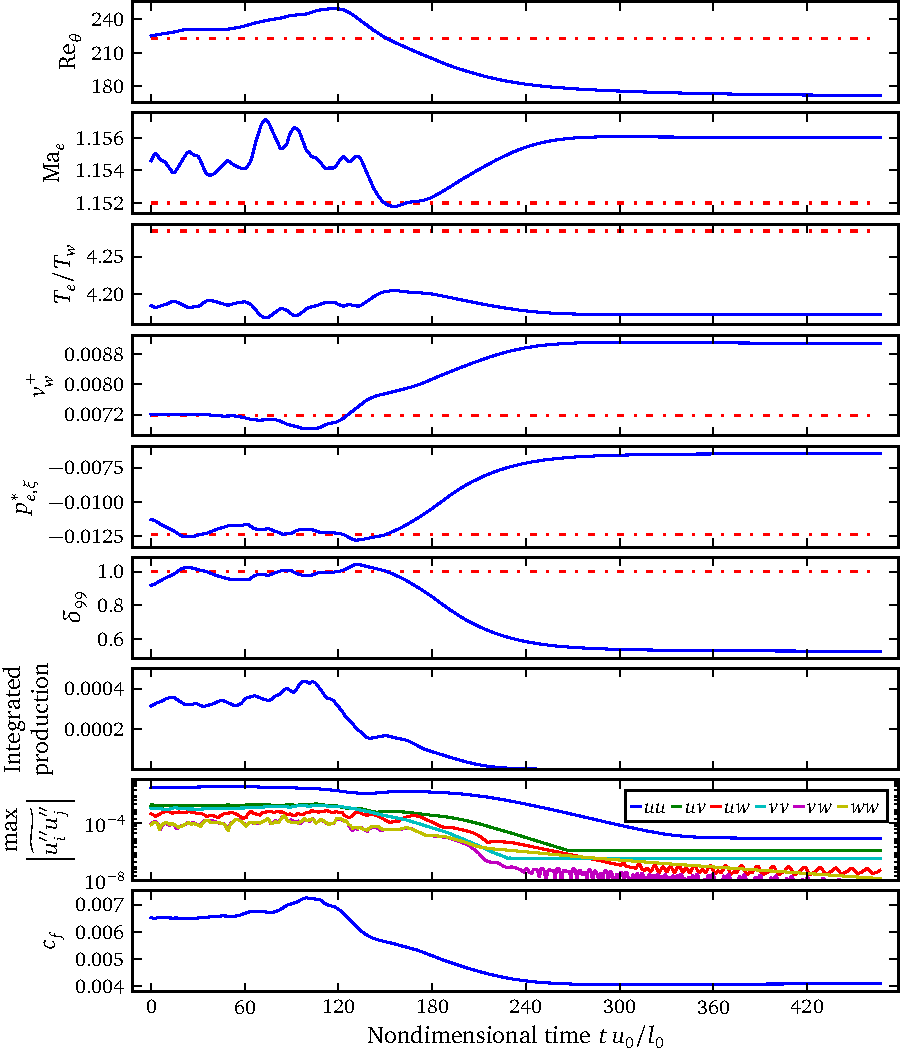
\includegraphics[height=0.99\textheight]{relam4134}
        \end{flushright}
    \end{column}
    \end{columns}
\end{frame}

%===============================================================================
\begin{frame}
    \frametitle{Location 3.199~m}
    \framesubtitle{$\Delta{}x^{+}\approx{}18.0$ and $\Delta{}z^{+}\approx{}10.8$}
    %
    \begin{columns}[c,onlytextwidth]
    \begin{column}{.35\linewidth}
        \scriptsize
        %
        Several intermittent\\dips in production
        \\\bigskip
        %
        Finally decays after\\O(36) eddy turnovers
    \end{column}
    \begin{column}{.65\linewidth}
        \vspace{-3.75em}
        \begin{flushright}
            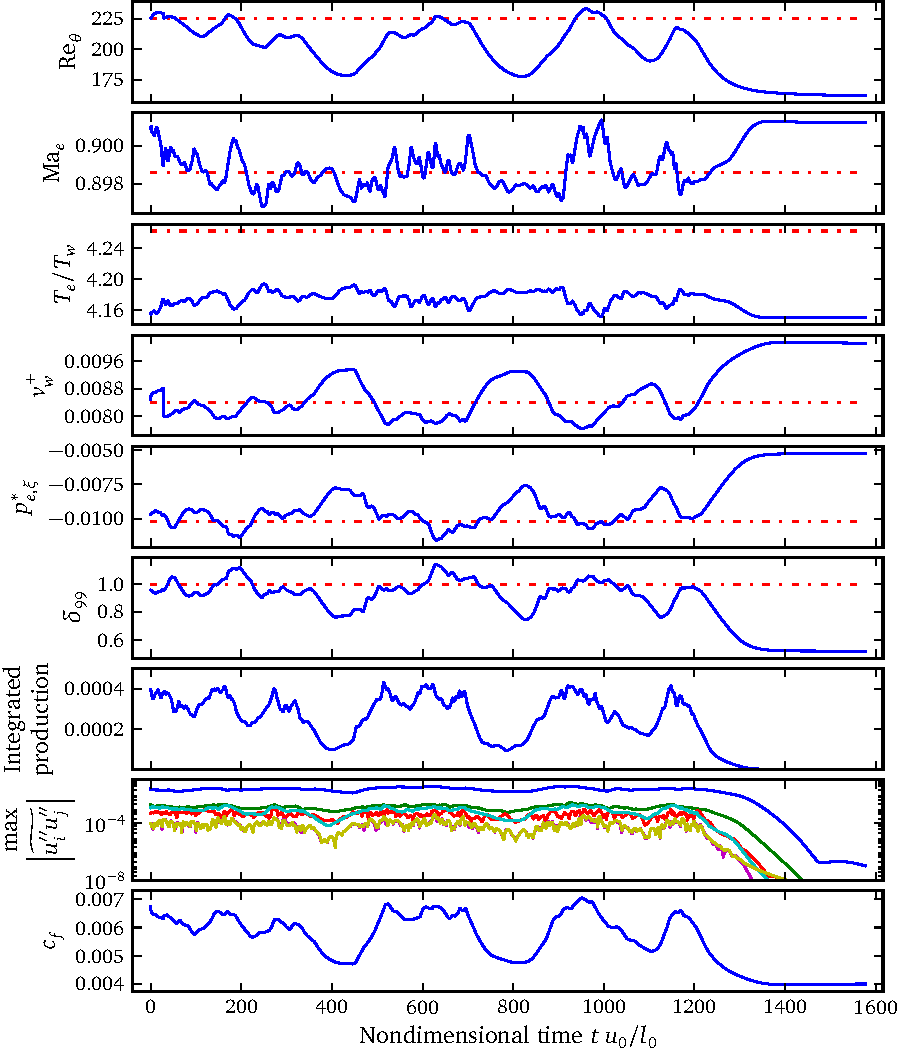
\includegraphics[height=0.99\textheight]{relam3199}
        \end{flushright}
    \end{column}
    \end{columns}
\end{frame}

%===============================================================================
\begin{frame}
    \frametitle{Location 2.299~m}
    \framesubtitle{$\Delta{}x^{+}\approx{}14.1$ and $\Delta{}z^{+}\approx{}8.5$}
    %
    \begin{columns}[c,onlytextwidth]
    \begin{column}{.35\linewidth}
        \scriptsize
        %
        Intermittent dips\\in production
        \\\bigskip
        %
        Sustains fluctuations for\\O(23) eddy turnovers
        \\\bigskip
        %
        $v_w^{+}$, $p_{e,\xi}^\ast$, and $\delta_{99}$ off target
    \end{column}
    \begin{column}{.65\linewidth}
        \vspace{-3.75em}
        \begin{flushright}
            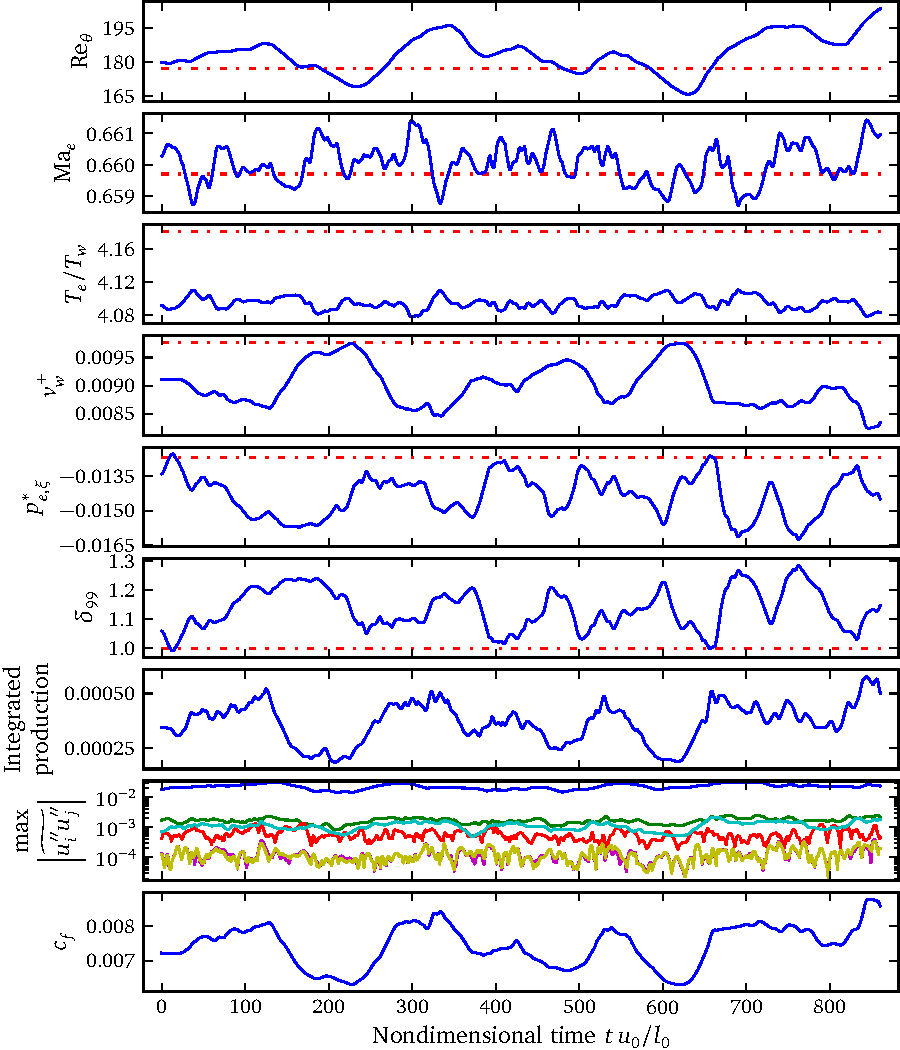
\includegraphics[height=0.99\textheight]{relam2299}
        \end{flushright}
    \end{column}
    \end{columns}
\end{frame}

%===============================================================================
\begin{frame}
    \frametitle{Location 2.299~m}
    \framesubtitle{$\Delta{}x^{+}\approx{}14.1$ and $\Delta{}z^{+}\approx{}8.5$\\
                   (Continued)}
    %
    \begin{columns}[c,onlytextwidth]
    \begin{column}{.35\linewidth}
        \scriptsize
        %
        Corrected $v_w^{+}$, $p_{e,\xi}^\ast$, and $\delta_{99}$
        \\\bigskip
        %
        Sustains fluctuations for\\another O(23) eddy turnovers
        \\\bigskip
        %
        What is this flow?
    \end{column}
    \begin{column}{.65\linewidth}
        \vspace{-5em}
        \begin{flushright}
            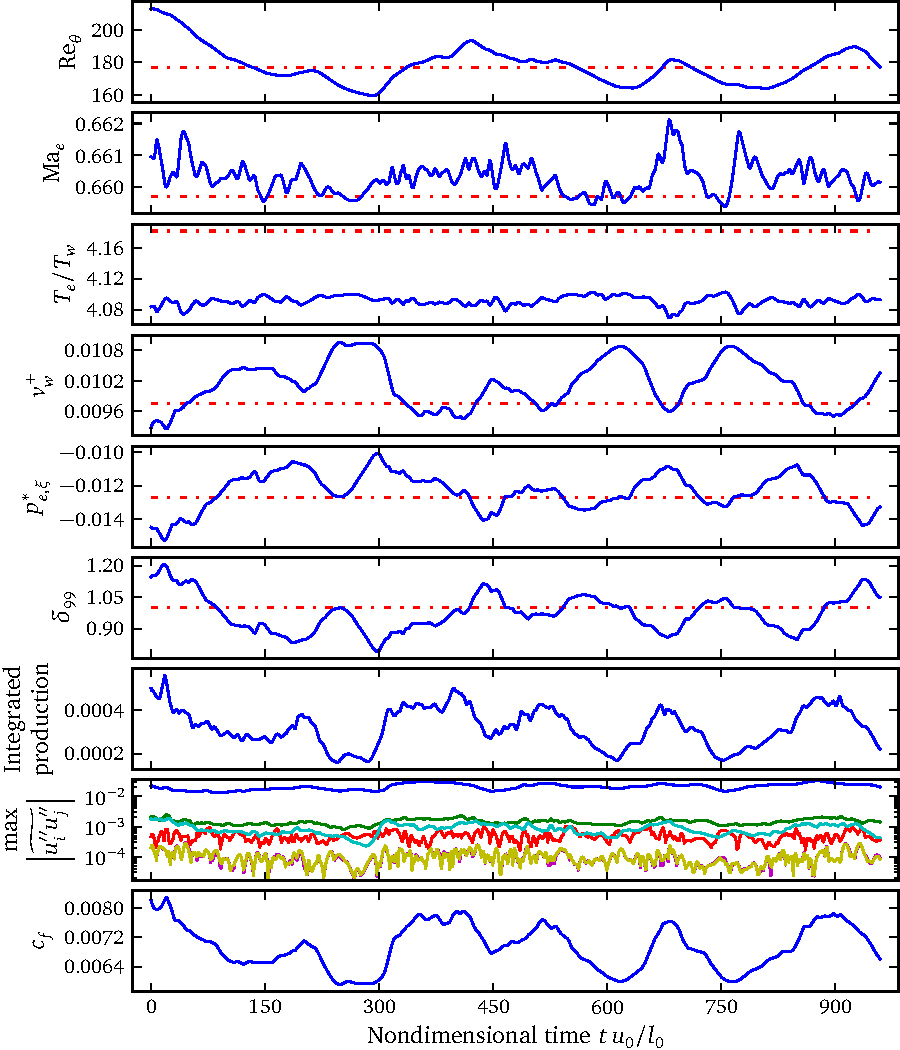
\includegraphics[height=0.99\textheight]{redux2299}
        \end{flushright}
    \end{column}
    \end{columns}
\end{frame}

%===============================================================================
\begin{frame}
    \frametitle{Assessing fluctuation-sustaining solution at 2.299~m}
    \framesubtitle{Well-resolved with large structures consistent w/ transitioning \& marginally turbulent flows}
    \begin{columns}
        \begin{column}{0.5\linewidth}
          \centering
          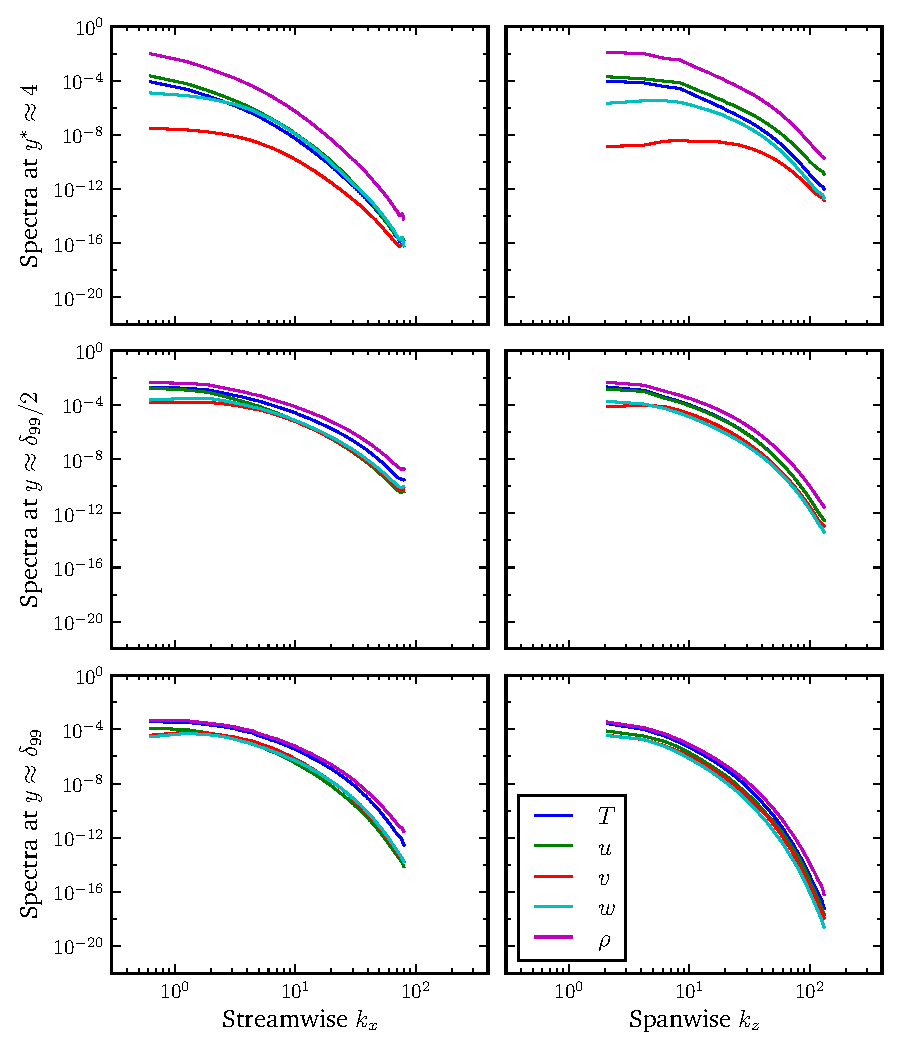
\includegraphics[width=\textwidth]{spectra-redux2299}
          \\\vspace{-0.5em}
          Spectra
        \end{column}
        \begin{column}{0.5\linewidth}
          \centering
          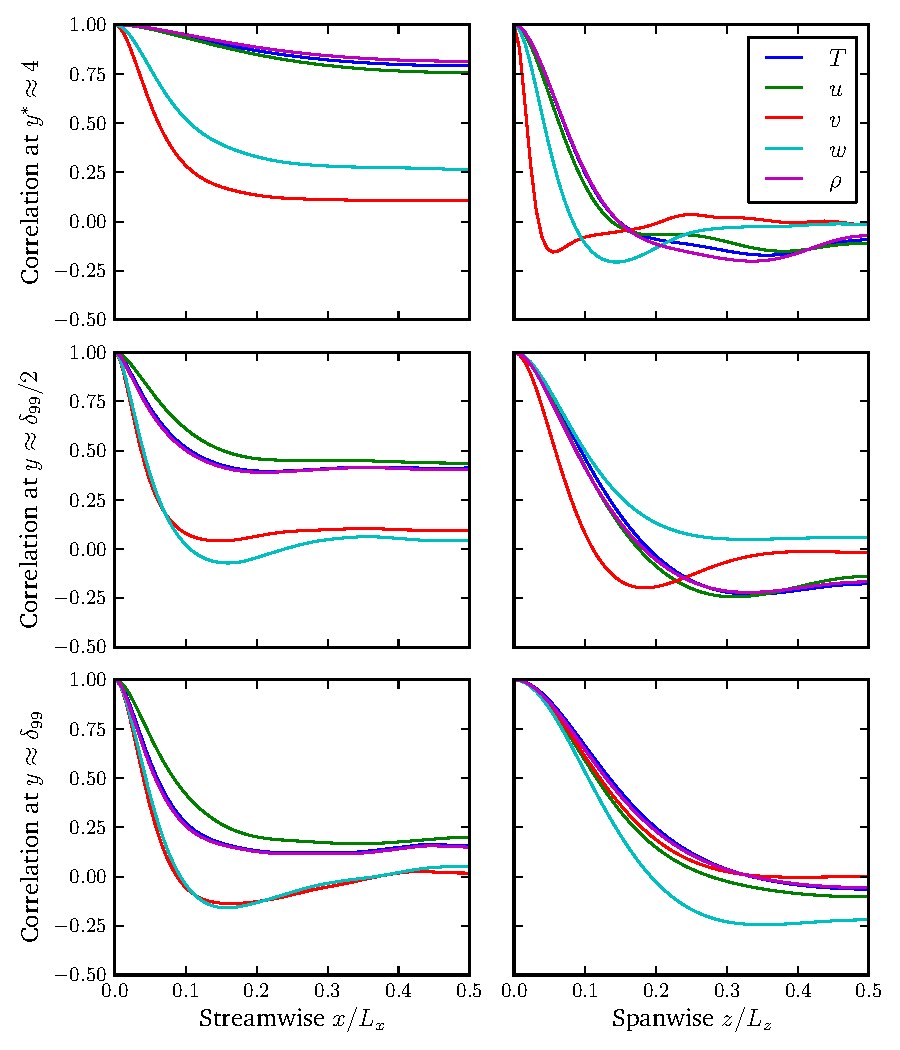
\includegraphics[width=\textwidth]{autocorr-redux2299}
          \\\vspace{-0.5em}
          Two-point correlations
        \end{column}
    \end{columns}
\end{frame}

%===============================================================================
\begin{frame}
    \frametitle{Location 1.389~m}
    \framesubtitle{$\Delta{}x^{+}\approx{}11.7$ and $\Delta{}z^{+}\approx{}7.0$}
    %
    \begin{columns}[c,onlytextwidth]
    \begin{column}{.35\linewidth}
        \scriptsize
        %
        Fluctuations decay in\\under 3.6 turnovers
    \end{column}
    \begin{column}{.65\linewidth}
        \vspace{-3.75em}
        \begin{flushright}
            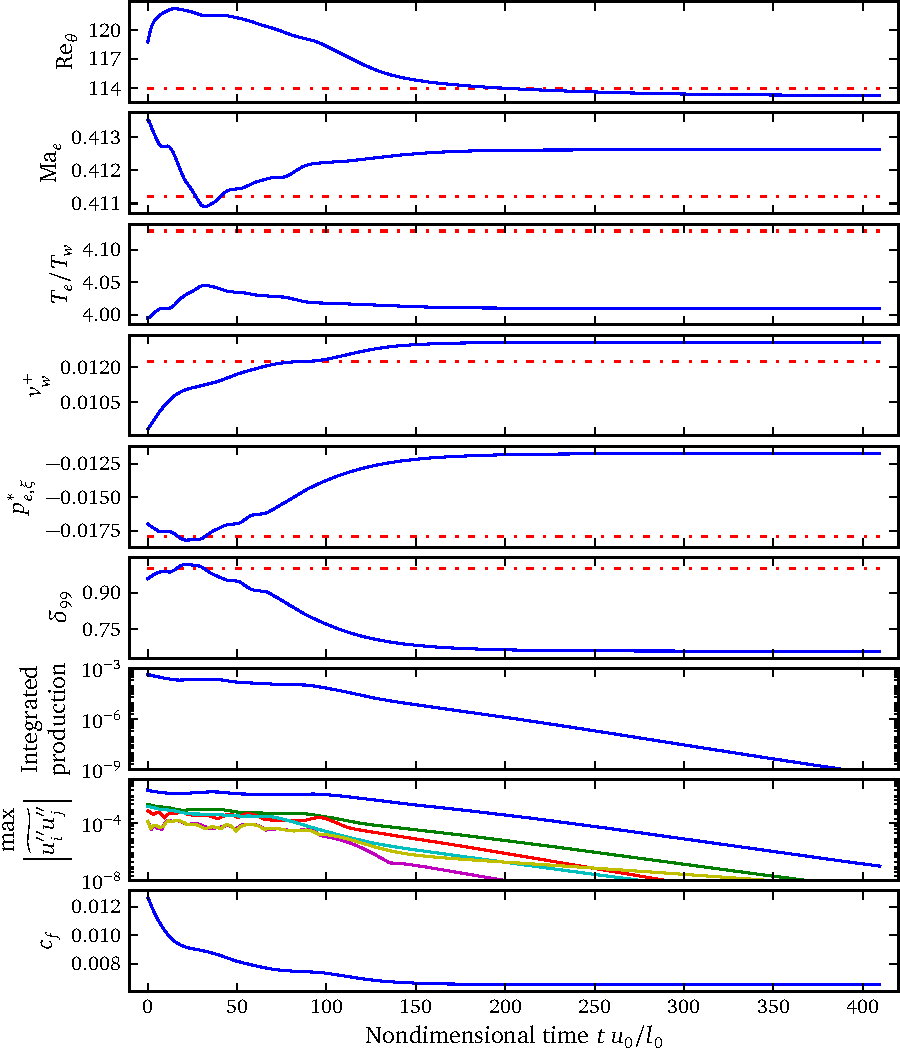
\includegraphics[height=0.99\textheight]{relam1389}
        \end{flushright}
    \end{column}
    \end{columns}
\end{frame}

%%%%%%%%%%%%%%%%%%%%%%%%%%%%%%%%%%%%%%%%%%%%%%%%%%%%%%%%%%%%%%%%%%%%%%%%%%%%%%%%
\subsection{Results: Fully Turbulent Initial Conditions}
%%%%%%%%%%%%%%%%%%%%%%%%%%%%%%%%%%%%%%%%%%%%%%%%%%%%%%%%%%%%%%%%%%%%%%%%%%%%%%%%

%===============================================================================
\begin{frame}
    \frametitle{Location 4.134~m}
    \framesubtitle{$\Delta{}x^{+}\approx{}17.2$ and $\Delta{}z^{+}\approx{}10.3$}
    %
    \begin{columns}[c,onlytextwidth]
    \begin{column}{.35\linewidth}
        \scriptsize
        Initialized with fully turbulent field from prior study simulation t4.134
        \\\bigskip
        %
        Changed $\mbox{Re}$ at $t=0$ so that $\mbox{Re}_\theta$ would be in
        vicinity of target value\\\bigskip
        %
        Relaminarized in O(10) turnovers
    \end{column}
    \begin{column}{.65\linewidth}
        \vspace{-3.75em}
        \begin{flushright}
            \includegraphics[height=0.99\textheight]{redux4134}
        \end{flushright}
    \end{column}
    \end{columns}
\end{frame}

%===============================================================================
\begin{frame}
    \frametitle{Location 3.199~m}
    \framesubtitle{$\Delta{}x^{+}\approx{}13.2$ and $\Delta{}z^{+}\approx{}7.9$}
    %
    \begin{columns}[c,onlytextwidth]
    \begin{column}{.35\linewidth}
        \scriptsize
        Initialized with fully turbulent field from prior study simulation t3.199
        \\\bigskip
        %
        Relaminarized in O(13) eddy turnovers
        \\\bigskip
        %
        Longer ``turbulent dwell'' than 4.134~m,
        likely because of weaker pressure gradient
        \\\bigskip
    \end{column}
    \begin{column}{.65\linewidth}
        \vspace{-3.75em}
        \begin{flushright}
            \includegraphics[height=0.99\textheight]{redux3199}
        \end{flushright}
    \end{column}
    \end{columns}
\end{frame}

%%%%%%%%%%%%%%%%%%%%%%%%%%%%%%%%%%%%%%%%%%%%%%%%%%%%%%%%%%%%%%%%%%%%%%%%%%%%%%%%
\subsection{Discussion}
%%%%%%%%%%%%%%%%%%%%%%%%%%%%%%%%%%%%%%%%%%%%%%%%%%%%%%%%%%%%%%%%%%%%%%%%%%%%%%%%

\begin{frame}

\begin{block}{Recapping the observations:}
\vspace{-0.5em}
\begin{itemize}
    \item Locations 4.134~m and 3.199~m\dots
        \begin{itemize}
            \item \dots{}relaminarized from ``admissible $v'$'' after 6 and 36 turnovers, respectively
            \item \dots{}relaminarized from turbulent initial conditions after 10 and 13 turnovers
        \end{itemize}
    \item Location  2.299~m sustained nontrivial fluctuations for 46 turnovers
    \item Location  1.389~m unable to sustain fluctuations
\end{itemize}
\end{block}

\pause{}
\begin{block}{Numerical experiments are a surrogate for noisy flight environment:}
\vspace{-0.5em}
\begin{itemize}
    \item Simulations are periodic--- perturbations never leave, only dissipate
    \item In flight, new perturbations continually arrive from upstream sources
\end{itemize}
\end{block}

\pause{}
\begin{block}{To conclude, a prediction:}
    \centering
    The turbulence-sustaining region is more than 1.389~m leeward of the Orion
    MPCV stagnation point during International Space Station
    return\pause\footnote{%
        Assuming the present homogenized flows capture
        the turbulence-sustaining behavior of spatially evolving boundary layers
        (not validated in present work)
    }
\end{block}

\end{frame}

%%%%%%%%%%%%%%%%%%%%%%%%%%%%%%%%%%%%%%%%%%%%%%%%%%%%%%%%%%%%%%%%%%%%%%%%%%%%%%%%
\section{Summary and Recommendations}
%%%%%%%%%%%%%%%%%%%%%%%%%%%%%%%%%%%%%%%%%%%%%%%%%%%%%%%%%%%%%%%%%%%%%%%%%%%%%%%%

%===============================================================================
\begin{frame}{Research Summary}
Reduced turbulence- and transition-driven uncertainty in aerothermodynamic
heating predictions for blunt-bodied reentry vehicles\ldots
\begin{enumerate}
 \item Through direct numerical simulation, provided high-quality
       homogenized turbulent boundary layer data possessing
   \begin{itemize}
     \item cold walls,
     \item wall blowing, and
     \item favorable pressure gradients
   \end{itemize}
       which reduces turbulence-driven predictive uncertainty by allowing
       more effective model calibration.
 \item Through examining a numerically accessible surrogate problem, reduced
       transition-driven uncertainty by providing new guidance about the regions
       on an ablative heat shield that should be modeled as turbulent--- without
       requiring perturbations in the flight environment to be well-characterized.
\end{enumerate}
\end{frame}

%===============================================================================
\begin{frame}{Future Work}
    \begin{enumerate}
     \item Further investigate the basic character of boundary layers
           simulated using \citet{Topalian2014Spatiotemporal}'s
           homogenization technique
           \begin{itemize}
               \item Tease apart cold wall, transpiration, pressure gradient effects
               \item Reduce homogenization to low Mach or incompressible limit
           \end{itemize}
     \item Recompute Orion MPCV solution tripping turbulence at
           location 1.389~m and compare predicted heat fluxes to measurements
           from NASA Exploration Flight Test~1 which launches in December 2014
     \item Examine scenario variants which do sustain turbulence, given
           fully turbulent initial conditions, to interrogate flow physics
           and assess parameter sensitivity
     \item Variety of DNS studies possible with current Suzerain capabilities, e.g.
         \begin{itemize}
            \item Supersonic, isothermal wall homogenized boundary layers
            \item Low Mach, homogenized boundary layers in adverse pressure gradients
         \end{itemize}
    \end{enumerate}
\end{frame}

%%%%===============================================================================
%%%\begin{frame}{Proposed Contributions Annotated by CSEM Area}
%%%\small
%%%\begin{description}[XX]
%%%\item[AB] Creation of manufactured solutions for the
%%%          relevant Navier–-Stokes formulation
%%%\item[B]  Creation of a new Fourier/B-spline pseudo-spectral channel code (``Suzerain'')
%%%\item[B]  Creation of a new parallel IO library for storing DNS simulation fields (``ESIO'')
%%%\item[B]  Creation of a library for auto-tuned parallel pencil decompositions (``underling'')
%%%\item[AB] Design of an uncertainty estimation procedure for autocorrelated turbulent statistics
%%%\item[C] Generation of low-Re compressible, isothermal channel statistics database
%%%\item[AB] Extension of Suzerain to temporally homogenized boundary layer problems
%%%\item[C] Generation of a temporally homogenized isothermal flat plate statistics database
%%%\item[AC] Creation of a relaminarization diagnostic for perturbation energy decay
%%%\item[BC] Characterization of the regions on an ablative TPS which can sustain turbulence
%%%\end{description}
%%%\end{frame}

%%%%%%%%%%%%%%%%%%%%%%%%%%%%%%%%%%%%%%%%%%%%%%%%%%%%%%%%%%%%%%%%%%%%%%%%%%%%%%%%
\appendix
%%%%%%%%%%%%%%%%%%%%%%%%%%%%%%%%%%%%%%%%%%%%%%%%%%%%%%%%%%%%%%%%%%%%%%%%%%%%%%%%

\begin{frame}{Backup}
\end{frame}

\begin{frame}
    \frametitle{Spectra for simulations t3.199 and t4.134}
    \framesubtitle{Compares favorably with \citet{Coleman1995Numerical} and \citet{Guarini2000Direct}}
    \begin{columns}
        \begin{column}{0.5\linewidth}
          \includegraphics[width=\textwidth]{spectra-turb3199}
        \end{column}
        \begin{column}{0.5\linewidth}
          \includegraphics[width=\textwidth]{spectra-turb4134}
        \end{column}
    \end{columns}
\end{frame}

\begin{frame}
    \frametitle{Two-point correlations for simulations t3.199 and t4.134}
    \framesubtitle{Compares favorably with \citet{Coleman1995Numerical} and \citet{Guarini2000Direct}}
    \begin{columns}
        \begin{column}{0.5\linewidth}
          \includegraphics[width=\textwidth]{autocorr-turb3199}
        \end{column}
        \begin{column}{0.5\linewidth}
          \includegraphics[width=\textwidth]{autocorr-turb4134}
        \end{column}
    \end{columns}
\end{frame}

\begin{frame}
    \frametitle{Momentum budgets for t3.199 (upper) and t4.134 (lower)}
    \begin{columns}
        \begin{column}{0.5\linewidth}
          \centering
          \includegraphics[width=\textwidth]{hqd_fans_rho_u}
          \\\vspace{-0.5em}
          Streamwise momentum, $\rho u$
        \end{column}
        \begin{column}{0.5\linewidth}
          \centering
          \includegraphics[width=\textwidth]{hqd_fans_rho_v}
          \\\vspace{-0.5em}
          Wall-normal momentum, $\rho v$
        \end{column}
    \end{columns}
\end{frame}


%%%%===============================================================================
%%%\begin{frame}{Quantitative comparison of centerline and wall means}
%%%             {Tabulated discrepancies between c03k15 and
%%%              CKM95a less than $1\%$, except $\Mach[\tau]\leq{}1.5\%$}
%%%\begin{table}
%%%\centering
%%%\resizebox{\textwidth}{!}{
%%%\begin{tabular}{c|ccccc|cccc}
%%%Identifier                               &
%%%$\textrm{Ma}_c$                          &
%%%$\textrm{Ma}_\tau$                       &
%%%$\textrm{Re}_c$                          &
%%%$\textrm{Re}_\tau$                       &
%%%$-\textrm{B}_q$                          &
%%%$\left<\rho_w\right>$                    &
%%%$\left<\rho_c\right>$                    &
%%%$\left<T_c\right>$                       &
%%%$\left<\mu_c\right>$
%%%\\
%%%\hline \hline
%%%%id     &  Mac    &  Matau  &  Rec   &  Retau  &  -Bq     &  rhow   &  rhoc    &  Tc     &  muc    \\
%%%c03k01  &  0.116  &  0.006  &  3489  &  190    &  0.0003  &  1.002  &  0.9999  &  1.002  &  1.001  \\
%%%c03k05  &  0.571  &  0.031  &  3391  &  193    &  0.0062  &  1.040  &  0.9973  &  1.043  &  1.028  \\
%%%\rowcolor{yellow}
%%%c03k15  &  1.493  &  0.081  &  2765  &  221    &  0.0491  &  1.365  &  0.9779  &  1.391  &  1.246  \\
%%%c03k30  &  2.240  &  0.120  &  1764  &  298    &  0.1500  &  2.450  &  0.9274  &  2.665  &  1.922  \\
%%%\hline
%%%c05k01  &  0.115  &  0.006  &  5758  &  297    &  0.0002  &  1.002  &  0.9999  &  1.002  &  1.001  \\
%%%c05k05  &  0.565  &  0.029  &  5598  &  303    &  0.0058  &  1.041  &  0.9979  &  1.042  &  1.028  \\
%%%c05k15  &  1.480  &  0.076  &  4595  &  348    &  0.0462  &  1.366  &  0.9834  &  1.385  &  1.242  \\
%%%c05k30  &  2.205  &  0.114  &  2973  &  472    &  0.1410  &  2.484  &  0.9486  &  2.600  &  1.891  \\
%%%\hline
%%%KMM87   &  0      &  0      &  3250  &  180    &  0       &  1      &  1       &  1      &  1      \\
%%%\rowcolor{yellow}
%%%CKM95a  &  1.502  &  0.082  &  2760  &  222    &  0.049   &  1.355  &  0.980   &  1.378  &  1.252  \\
%%%CKM95b  &  2.225  &  0.116  &  2872  &  451    &  0.137   &  2.388  &  0.952   &  2.490  &  1.894  \\
%%%\end{tabular}
%%%}%resizebox
%%%\end{table}
%%%\vfill
%%%\begin{footnotesize}\begin{flushright}
%%%CKM95\{a,b\} reproduced from \citet{Coleman1995Numerical}\\
%%%Incompressible results from \citet{Kim1987Turbulence}
%%%\end{flushright}\end{footnotesize}
%%%\end{frame}
%%%
%%%%===============================================================================
%%%\begin{frame}{On computing uncertainty due to finite sample sizes}
%%%\vspace{-2em}
%%%\begin{columns}
%%%  \begin{column}{.50\linewidth}
%%%    \includegraphics[width=0.99\linewidth]{ChannelSchematic}
%%%  \end{column}
%%%  \begin{column}{.50\linewidth}
%%%    \includegraphics[width=0.99\linewidth]{bar_u__y}
%%%  \end{column}
%%%\end{columns}
%%%\vspace{-2em}
%%%\begin{center}
%%%  \includegraphics{Re_tau}
%%%\end{center}
%%%\end{frame}
%%%
%%%%===============================================================================
%%%\begin{frame}{Estimating effective sample size using autocorrelation}
%%%\begin{itemize}
%%%  \item Estimate variances from data with \emph{a priori} unknown
%%%        autocorrelations
%%%  \item Many practitioners downsample, compute from independent data:
%%%  \begin{itemize}
%%%    \item ``Just enough'' downsampling always discards valuable information
%%%    \item Objectively downsample 1000s of signals with distinct signatures?
%%%  \end{itemize}
%%%  \item Effective sample size techniques applicable
%%%        but require autocorrelation function $\rho$, e.g.
%%%%
%%%$$
%%%  \operatorname{Var} \bar{X}
%%%  =
%%%  \frac{\sigma_X^2}{N_\text{effective}}
%%%  =
%%%  \frac{\frac{N}{N-T_0} s_X^2}{\frac{N}{T_0}}
%%%  =
%%%  \frac{T_0}{N\left(N-T_0\right)} \sum_{i=1}^{N} \left(X_i - \bar{X}\right)^2
%%%$$
%%%$$
%%%  T_0 = 1+2\sum_{k=1}^{N-1} \left(1-\frac{k}{N}\right) \operatorname{\rho}(k)
%%%$$
%%%%
%%%  \item Direct estimates of $\operatorname{\rho}(k)$
%%%        from O(100) samples are unsatisfyingly noisy
%%%\end{itemize}
%%%\end{frame}
%%%
%%%%===============================================================================
%%%\begin{frame}{Maximum entropy autocorrelation estimates}
%%%Estimating a smoothed $\operatorname{\rho}$ using AR(p)
%%%processes is natural and efficient:
%%%\begin{align}
%%%  X_n + a_1 X_{n - 1} + \dots + a_p X_{n - p} &= \epsilon_n
%%%  &
%%%  \epsilon_n &\sim{} N\left(0, \sigma^2_\epsilon\right)
%%%\intertext{
%%%which implies
%%%}
%%%  \sigma^2_X \left(
%%%      \rho_0 + a_1 \rho_{1} + \dots + a_p \rho_{p}
%%%  \right) &= \sigma^2_\epsilon
%%%  &
%%%  \rho_0 &= 1
%%%\\
%%%  \rho_k + a_1 \rho_{k-1} + \dots + a_p \rho_{k-p} &= 0
%%%  &
%%%  k &\geq{} p
%%%\end{align}
%%%\vspace{-1.5em}
%%%\begin{itemize}
%%%  \item For a given order $p$, fitting an AR(p) model
%%%        is \emph{maximum entropy} under practically no
%%%        assumptions~\citep{Choi1984Informationtheoretic}
%%%  \item An optimal $p$ may be found using information theoretic,
%%%        finite sample model selection criteria~\citep{Broersen2000Finite}
%%%  \item Computing all candidates and selecting the best one
%%%        requires only O($N^2$) FLOPs on O($N^2$) storage~\citep{Durbin1960,Burg1975}
%%%  \item Header-only C++ implementation: \url{http://rhysu.github.com/ar/}\\
%%%        Standalone command line and GNU Octave functionality provided
%%%\end{itemize}
%%%\end{frame}
%%%
%%%%===============================================================================
%%%\begin{frame}{The optimal model for $\text{Re}_\tau$ is AR(2) according to CIC}
%%%\begin{center}
%%%  \includegraphics{realizations}\\
%%%  \vfill
%%%  \includegraphics{autocor}
%%%\end{center}
%%%\end{frame}
%%%
%%%%===============================================================================
%%%\begin{frame}{\citet{Settles1991Hypersonic}'s criteria for assessing data}
%%%\vfill
%%%%\begin{small}
%%%%``\dots{}looking for those few experimental studies of unimpeachable
%%%%quality\dots''
%%%%\end{small}
%%%\begin{columns}[t]
%%%  \begin{column}{.47\linewidth}
%%%    \begin{block}{Necessary criteria}
%%%      \begin{enumerate}
%%%        \item Baseline  applicability
%%%        \item {\color<1->{red} Simplicity}
%%%        \item Specific applicability
%%%        \item {\color<1->{red} Well-defined experimental boundary conditions}
%%%        \item Well-defined experimental error bounds
%%%        \item Consistency
%%%        \item Adequate documentation
%%%        \item Adequate spatial resolution
%%%      \end{enumerate}
%%%    \end{block}
%%%  \end{column}
%%%  \begin{column}{.47\linewidth}
%%%    \begin{block}{Desirable criteria}
%%%      \begin{enumerate}
%%%        \item {\color<1->{red} Turbulent data}
%%%        \item {\color<1->{red} Realistic test conditions}
%%%        \item Non-intrusive instrumentation
%%%        \item Redundant measurements
%%%        \item Flow structure and physics
%%%      \end{enumerate}
%%%    \end{block}
%%%  \end{column}
%%%\end{columns}
%%%\end{frame}
%%%
%%%%===============================================================================
%%%\begin{frame}{\citet{Spalart1988Direct}'s periodic boundary layer formulation I}
%%%\begin{center}
%%%  \includegraphics[width=0.65\textwidth]{Spalart1988Figure1a}
%%%\end{center}
%%%\begin{itemize}
%%%\begin{footnotesize}
%%%  \item Observed layer thickness and energy have a slowly varying signal in $x$
%%%  \item Defined $\eta$ so boundary \&
%%%        viscous sublayer thickness independent of $x$, i.e.
%%%        \begin{align*}
%%%          u(x,\eta, z, t) &= U(x,\eta) + A(x,\eta)u_p(x,\eta,z,t)
%%%        \end{align*}
%%%        where
%%%        \begin{align*}
%%%          U(x,\eta) &\equiv \left< u(x,\eta,z,t) \right>_{z,t}
%%%          \\
%%%          U'(x,\eta,z,t) &\equiv u(x,\eta,z,t) - U(x,\eta)
%%%          \\
%%%          A(x,\eta) &\propto \left< {U'(x,\eta,z,t)}^2 \right>_{z,t}^{1/2}
%%%        \end{align*}
%%%\end{footnotesize}
%%%\end{itemize}
%%%\end{frame}
%%%
%%%%===============================================================================
%%%\begin{frame}{\citet{Spalart1988Direct}'s periodic boundary layer formulation II}
%%%\begin{center}
%%%  \includegraphics[width=0.65\textwidth]{Spalart1988Figure1a}
%%%\end{center}
%%%\begin{itemize}
%%%\begin{footnotesize}
%%%\item Assumed $u_p(x,\eta,z,t)$'s scales vary
%%%      insignificantly compared to $U(x,\eta)$, $A(x,\eta)$
%%%\item By assumptions  $u_p$ is periodic, $\left< u_p \right>_{z,t}=0$,
%%%      and $\left<{u_p'}^2\right>_{z,t}^{1/2}$ is independent of $x$
%%%\item By chain rule, $\frac{\partial{}u}{\partial{}x} =
%%%            \underbrace{
%%%              \frac{\partial{}U}{\partial{}x}
%%%              + \frac{\partial{}A}{\partial{}x} u_p
%%%            }_{\mbox{slow terms}}
%%%          \,
%%%          + \underbrace{
%%%              A \frac{\partial{}u_p}{\partial{}x}
%%%            }_{\mbox{fast term}}$
%%%\item Used $u_\tau/U_\infty\to{}0$ as $\Reynolds{}\to\infty$
%%%      and multiscale analysis to add ``slow growth
%%%      terms''
%%%\end{footnotesize}
%%%\end{itemize}
%%%\end{frame}
%%%
%%%%===============================================================================
%%%\begin{frame}{\citet{Spalart1988Direct}'s periodic boundary layer formulation III}
%%%\begin{center}
%%%  \includegraphics[width=0.65\textwidth]{Spalart1988Figure1a}
%%%\end{center}
%%%\begin{itemize}
%%%\item Spalart needed slow growth information to close the
%%%      new terms:
%%%  \begin{itemize}
%%%    \item Chose to simulate a sequence of ''stations'' along the
%%%          boundary layer
%%%    \item Each stations' details fixed by the preceding upstream station
%%%    \item In incompressible case, only mean-velocity and Reynolds
%%%          stress profile information required from upstream
%%%  \end{itemize}
%%%\item \citet{Guarini2000Direct} extended technique to the compressible
%%%      case
%%%\item Sadly, this is not an entirely realistic boundary layer
%%%\end{itemize}
%%%\end{frame}
%%%
%%%%===============================================================================
%%%\begin{frame}{Spatially evolving boundary layer simulations are difficult}
%%%%
%%%Reentry scenario is accessible by DNS:
%%%$\Reynolds[\theta]\approx\left[300,700\right]$,
%%%$\Mach[e]\approx\left[.8,1.6\right]$
%%%%
%%%\vfill
%%%%
%%%\citet{Schlatter2010Assessment} assessed low-\Reynolds{} boundary layer simulations:
%%%\footnote{
%%%    \citet{Spalart1988Direct, Komminaho2002Reynolds, Khujadze2007New,
%%%    Khujadze2004DNS, Ferrante2005Reynolds, Simens2009Highresolution,
%%%    Wu2009Direct, Schlatter2009High, Schlatter2009Turbulent}
%%%}
%%%\begin{itemize}
%%%  \item Incompressible, zero-pressure-gradient, flat-plate boundary layer
%%%  \item ``\dots{}surprisingly inconsistent
%%%        predictions for quantities as basic as the friction coefficient, shape
%%%        factor, and fluctuation maxima.''
%%%  \item All used ``reliable numerical methods with sufficiently high resolutions''
%%%  \item Concluded discrepancies stemmed from differences in setup:
%%%  \begin{itemize}
%%%    \item Inflow Reynolds number and turbulence generation
%%%    \item Sufficient settling length to reach final turbulent state
%%%    \item Box dimensions and boundary conditions (e.g. pressure gradients)
%%%  \end{itemize}
%%%\end{itemize}
%%%%
%%%\end{frame}
%%%
%%%%===============================================================================
%%%\begin{frame}{Temporally homogenized boundary layers in a nutshell}
%%%%
%%%\begin{columns}
%%%\begin{column}{0.75\linewidth}
%%%\begin{block}{Motivating flow: Rayleigh problem}
%%%At $t=0$, impulsively start infinite plate with velocity $v$\\
%%%Homogeneous in space but \emph{not} temporally stationary
%%%\end{block}
%%%\end{column}
%%%\begin{column}{0.23\linewidth}
%%%\center{\includegraphics[width=0.99\linewidth]{rayleigh_cartoon.pdf}}
%%%\end{column}
%%%\end{columns}
%%%%
%%%\vspace{1em}
%%%%
%%%Starting from N.--S., $\pp{U}{t} + N[U] = 0$,
%%%define $t_f = t$, $t_s = \epsilon t$ for $\epsilon \ll 1$
%%%%
%%%\vspace{1em}
%%%%
%%%Assume mean and RMS depend on $t_s$; self-similarity $\eta = y/\Delta[t_s]$:
%%%\begin{align}
%%% U[x,y,z,t] &= \underbrace{\overline{U}[y, t_s]}_{U_{\infty}[t_s] F\left[\eta\right]}
%%%             + \underbrace{U_{\text{RMS}}[y, t_s]}_{U_{\text{RMS},A}[t_s] G\left[\eta\right]}
%%%               U'[x,y,z,t_f]
%%%\end{align}
%%%%
%%%Under these assumptions one can show
%%%\begin{align}
%%%  \pp{U}{t_f} + N[U] = - \epsilon \pp{U}{t_s}
%%%  &=
%%%  - \frac{U}{U_{\infty}} \pp{U_{\infty}}{t_s}
%%%  + \pp{\Delta}{t_s} \frac{y}{\Delta} \left(
%%%      \pp{\overline{U}}{y} + \frac{U'}{U_{\text{RMS}}} \pp{U_{\text{RMS}}}{y}
%%%    \right)
%%%\end{align}
%%%%
%%%\end{frame}
%%%
%%%%===============================================================================
%%%\begin{frame}{Spatial discretization}
%%%\begin{center}
%%%  \includegraphics[width=.8\linewidth]{Kwok2001BsplineModifiedWavenumbers}
%%%\end{center}
%%%\vfill
%%%\begin{block}{Basis and method choices}
%%%  \begin{itemize}
%%%    \item Fourier Galerkin in streamwise, spanwise directions
%%%    \item B-spline collocation in wall-normal direction
%%%  \end{itemize}
%%%\end{block}
%%%\end{frame}
%%%

%===============================================================================
%\nocite{SomeReference} % TODO
\begin{frame}[allowframebreaks]
  \fontsize{5.5pt}{6.0}\selectfont
  \bibliographystyle{plainnat}
  \bibliography{references}
\end{frame}

%%%%%%%%%%%%%%%%%%%%%%%%%%%%%%%%%%%%%%%%%%%%%%%%%%%%%%%%%%%%%%%%%%%%%%%%%%%%%%
\end{document}
